\documentclass[14pt]{beamer}

% Presento style file
\usepackage{config/presento}
\usepackage{amsmath}
\usepackage{amssymb}
\usepackage{tcolorbox}

\usepackage{physics}
\usepackage{amsmath}
\usepackage{tikz}
\usepackage{mathdots}
\usepackage{yhmath}
\usepackage{cancel}
\usepackage{color}
\usepackage{siunitx}
\usepackage{array}
\usepackage{multirow}
\usepackage{amssymb}
\usepackage{gensymb}
\usepackage{tabularx}
\usepackage{extarrows}
\usepackage{booktabs}
\usetikzlibrary{fadings}
\usetikzlibrary{patterns}
\usetikzlibrary{shadows.blur}
\usetikzlibrary{shapes}

% custom command and packages
% custom packages
\usepackage{textpos}
\setlength{\TPHorizModule}{1cm}
\setlength{\TPVertModule}{1cm}

\newcommand\crule[1][black]{\textcolor{#1}{\rule{2cm}{2cm}}}



% Information
\title{Is Cover Of a Cover another Cover?}
\subtitle{}
\author{Aakash Ghosh}
\institute{19MS129}
\date{$1^{st}$ November, 2022}

\begin{document}

% Title page
\begin{frame}[plain]
\maketitle
\end{frame}

% sections in the presentation
\begin{frame}{The Question}    
    \begin{tcolorbox}[colframe=colororange, colback=colororange!10,]
            Let $\phi:Y\to X$ be a covering of $X$ by $Y$ and let $\psi:Z\to Y$ be a covering of $Y$ by $Z$. Is $\phi\circ\psi:Z\to X$ a covering of $X$ by $Z$?
    \end{tcolorbox}\pause
    The short answer is \textcolor{colororange}{NO}\pause. We show this by taking $X$ to be the Hawaiian earring and constructing $Y$ and $Z$ appropiately. 
\end{frame}




\framecard[colorgreen]{{\color{white}\hugetext{The topology of Hawaiian Earring}}}

\begin{frame}{The construction of the space}
    We define \textcolor{colororange}{$C_n=\left\{z:\left|z-\frac{i}{2n}\right|=1/2n,z\in\mathbb C\right\}$}\pause. The Hawaiian Earring is defined as \textcolor{colororange}{$$H=C_1$$}
    \begin{center}
        

\tikzset{every picture/.style={line width=0.75pt}} %set default line width to 0.75pt        

\begin{tikzpicture}[x=0.75pt,y=0.75pt,yscale=-1,xscale=1]
%uncomment if require: \path (0,300); %set diagram left start at 0, and has height of 300

%Flowchart: Connector [id:dp6190573425763748] 
\draw  [color={rgb, 255:red, 245; green, 166; blue, 35 }  ,draw opacity=1 ] (180,220) .. controls (180,186.86) and (206.86,160) .. (240,160) .. controls (273.14,160) and (300,186.86) .. (300,220) .. controls (300,253.14) and (273.14,280) .. (240,280) .. controls (206.86,280) and (180,253.14) .. (180,220) -- cycle ;




\end{tikzpicture}

    \end{center}
\end{frame}



\begin{frame}{The construction of Hawaiian Earring}
    We define \textcolor{colororange}{$C_n=\left\{z:\left|z-\frac{i}{n}\right|=1/n,z\in\mathbb{C}\right\}$}. The Hawaiian Earring is defined as \textcolor{colororange}{$$H=C_1\cup C_2$$}
    \begin{center}
        

\tikzset{every picture/.style={line width=0.75pt}} %set default line width to 0.75pt        

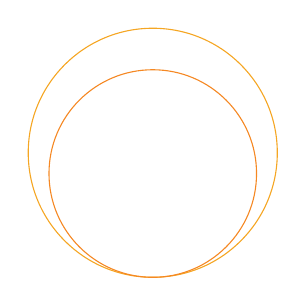
\begin{tikzpicture}[x=0.75pt,y=0.75pt,yscale=-1,xscale=1]
%uncomment if require: \path (0,300); %set diagram left start at 0, and has height of 300

%Flowchart: Connector [id:dp6190573425763748] 
\draw  [color={rgb, 255:red, 245; green, 166; blue, 35 }  ,draw opacity=1 ] (180,220) .. controls (180,186.86) and (206.86,160) .. (240,160) .. controls (273.14,160) and (300,186.86) .. (300,220) .. controls (300,253.14) and (273.14,280) .. (240,280) .. controls (206.86,280) and (180,253.14) .. (180,220) -- cycle ;
%Flowchart: Connector [id:dp7012306874990505] 
\draw  [color={rgb, 255:red, 245; green, 136; blue, 35 }  ,draw opacity=1 ] (190,230) .. controls (190,202.39) and (212.39,180) .. (240,180) .. controls (267.61,180) and (290,202.39) .. (290,230) .. controls (290,257.61) and (267.61,280) .. (240,280) .. controls (212.39,280) and (190,257.61) .. (190,230) -- cycle ;




\end{tikzpicture}

    \end{center}
\end{frame}



\begin{frame}{The construction of Hawaiian Earring}
    We define \textcolor{colororange}{$C_n=\left\{z:\left|z-\frac{i}{2n}\right|=1/2n,x\in\mathbb{C}\right\}$}. The Hawaiian Earring is defined as \textcolor{colororange}{$$H=C_1\cup C_2\cup C_3$$}
    \begin{center}
        

\tikzset{every picture/.style={line width=0.75pt}} %set default line width to 0.75pt        

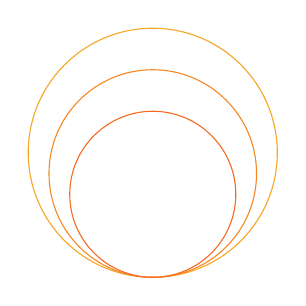
\begin{tikzpicture}[x=0.75pt,y=0.75pt,yscale=-1,xscale=1]
%uncomment if require: \path (0,300); %set diagram left start at 0, and has height of 300

%Flowchart: Connector [id:dp6190573425763748] 
\draw  [color={rgb, 255:red, 245; green, 166; blue, 35 }  ,draw opacity=1 ] (180,220) .. controls (180,186.86) and (206.86,160) .. (240,160) .. controls (273.14,160) and (300,186.86) .. (300,220) .. controls (300,253.14) and (273.14,280) .. (240,280) .. controls (206.86,280) and (180,253.14) .. (180,220) -- cycle ;
%Flowchart: Connector [id:dp7012306874990505] 
\draw  [color={rgb, 255:red, 245; green, 136; blue, 35 }  ,draw opacity=1 ] (190,230) .. controls (190,202.39) and (212.39,180) .. (240,180) .. controls (267.61,180) and (290,202.39) .. (290,230) .. controls (290,257.61) and (267.61,280) .. (240,280) .. controls (212.39,280) and (190,257.61) .. (190,230) -- cycle ;
%Flowchart: Connector [id:dp8115238254891972] 
\draw  [color={rgb, 255:red, 245; green, 106; blue, 35 }  ,draw opacity=1 ] (200,240) .. controls (200,217.91) and (217.91,200) .. (240,200) .. controls (262.09,200) and (280,217.91) .. (280,240) .. controls (280,262.09) and (262.09,280) .. (240,280) .. controls (217.91,280) and (200,262.09) .. (200,240) -- cycle ;




\end{tikzpicture}

    \end{center}
\end{frame}



\begin{frame}{The construction of the Hawaiian Earring}
    We define \textcolor{colororange}{$C_n=\left\{z:\left|z-\frac{1}{2n}\right|=1/2n\right\}$}. The Hawaiian Earring is defined as \textcolor{colororange}{$$H=\bigcup_{n\in\mathbb N}C_n$$}
    \begin{center}
        

\tikzset{every picture/.style={line width=0.75pt}} %set default line width to 0.75pt        

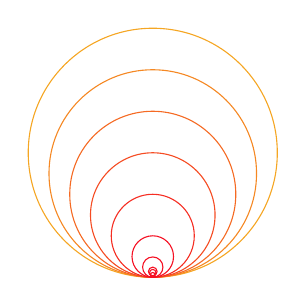
\begin{tikzpicture}[x=0.75pt,y=0.75pt,yscale=-1,xscale=1]
%uncomment if require: \path (0,300); %set diagram left start at 0, and has height of 300

%Flowchart: Connector [id:dp6190573425763748] 
\draw  [color={rgb, 255:red, 245; green, 166; blue, 35 }  ,draw opacity=1 ] (180,220) .. controls (180,186.86) and (206.86,160) .. (240,160) .. controls (273.14,160) and (300,186.86) .. (300,220) .. controls (300,253.14) and (273.14,280) .. (240,280) .. controls (206.86,280) and (180,253.14) .. (180,220) -- cycle ;
%Flowchart: Connector [id:dp7012306874990505] 
\draw  [color={rgb, 255:red, 245; green, 136; blue, 35 }  ,draw opacity=1 ] (190,230) .. controls (190,202.39) and (212.39,180) .. (240,180) .. controls (267.61,180) and (290,202.39) .. (290,230) .. controls (290,257.61) and (267.61,280) .. (240,280) .. controls (212.39,280) and (190,257.61) .. (190,230) -- cycle ;
%Flowchart: Connector [id:dp8115238254891972] 
\draw  [color={rgb, 255:red, 245; green, 106; blue, 35 }  ,draw opacity=1 ] (200,240) .. controls (200,217.91) and (217.91,200) .. (240,200) .. controls (262.09,200) and (280,217.91) .. (280,240) .. controls (280,262.09) and (262.09,280) .. (240,280) .. controls (217.91,280) and (200,262.09) .. (200,240) -- cycle ;
%Flowchart: Connector [id:dp13256721831630391] 
\draw  [color={rgb, 255:red, 245; green, 76; blue, 35 }  ,draw opacity=1 ] (210,250) .. controls (210,233.43) and (223.43,220) .. (240,220) .. controls (256.57,220) and (270,233.43) .. (270,250) .. controls (270,266.57) and (256.57,280) .. (240,280) .. controls (223.43,280) and (210,266.57) .. (210,250) -- cycle ;
%Flowchart: Connector [id:dp6922226533803466] 
\draw  [color={rgb, 255:red, 245; green, 46; blue, 35 }  ,draw opacity=1 ] (220,260) .. controls (220,248.95) and (228.95,240) .. (240,240) .. controls (251.05,240) and (260,248.95) .. (260,260) .. controls (260,271.05) and (251.05,280) .. (240,280) .. controls (228.95,280) and (220,271.05) .. (220,260) -- cycle ;
%Flowchart: Connector [id:dp24338136998325388] 
\draw  [color={rgb, 255:red, 245; green, 16; blue, 35 }  ,draw opacity=1 ] (230,270) .. controls (230,264.48) and (234.48,260) .. (240,260) .. controls (245.52,260) and (250,264.48) .. (250,270) .. controls (250,275.52) and (245.52,280) .. (240,280) .. controls (234.48,280) and (230,275.52) .. (230,270) -- cycle ;
%Flowchart: Connector [id:dp8937826625032416] 
\draw  [color={rgb, 255:red, 245; green, 16; blue, 35 }  ,draw opacity=1 ] (235.1,275.1) .. controls (235.1,272.39) and (237.29,270.2) .. (240,270.2) .. controls (242.71,270.2) and (244.9,272.39) .. (244.9,275.1) .. controls (244.9,277.81) and (242.71,280) .. (240,280) .. controls (237.29,280) and (235.1,277.81) .. (235.1,275.1) -- cycle ;
%Flowchart: Connector [id:dp5500717722497827] 
\draw  [color={rgb, 255:red, 245; green, 16; blue, 35 }  ,draw opacity=1 ] (237.9,277.2) .. controls (237.9,276.04) and (238.84,275.1) .. (240,275.1) .. controls (241.16,275.1) and (242.1,276.04) .. (242.1,277.2) .. controls (242.1,278.36) and (241.16,279.3) .. (240,279.3) .. controls (238.84,279.3) and (237.9,278.36) .. (237.9,277.2) -- cycle ;
%Flowchart: Connector [id:dp539739836015123] 
\draw  [color={rgb, 255:red, 245; green, 16; blue, 35 }  ,draw opacity=1 ] (238.45,277.75) .. controls (238.45,276.89) and (239.14,276.2) .. (240,276.2) .. controls (240.86,276.2) and (241.55,276.89) .. (241.55,277.75) .. controls (241.55,278.61) and (240.86,279.3) .. (240,279.3) .. controls (239.14,279.3) and (238.45,278.61) .. (238.45,277.75) -- cycle ;
%Flowchart: Connector [id:dp7581584436234312] 
\draw  [color={rgb, 255:red, 245; green, 16; blue, 35 }  ,draw opacity=1 ] (238.85,278.85) .. controls (238.85,278.21) and (239.36,277.7) .. (240,277.7) .. controls (240.64,277.7) and (241.15,278.21) .. (241.15,278.85) .. controls (241.15,279.49) and (240.64,280) .. (240,280) .. controls (239.36,280) and (238.85,279.49) .. (238.85,278.85) -- cycle ;




\end{tikzpicture}

    \end{center}
\end{frame}


\begin{frame}{The topology of the Hawaiian Earring}
    We give the Hawaiian Earring the subspace topology. In particular, we look at how small open sets around points looks like and build a sub-basis.\pause
    \begin{center}
        


\tikzset{every picture/.style={line width=0.75pt}} %set default line width to 0.75pt        

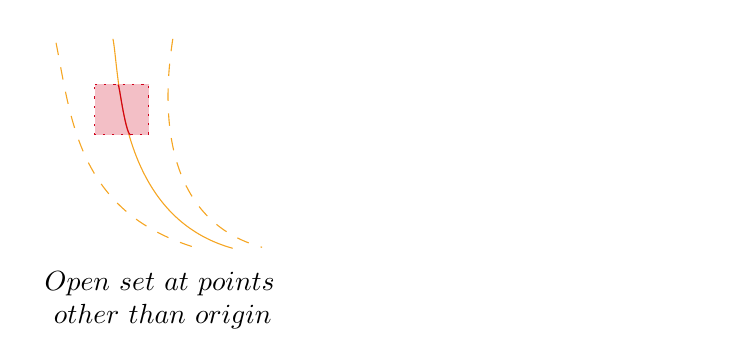
\begin{tikzpicture}[x=0.75pt,y=0.75pt,yscale=-1,xscale=1]
%uncomment if require: \path (0,300); %set diagram left start at 0, and has height of 300

%Flowchart: Connector [id:dp6190573425763748] 
\draw  [color={rgb, 255:red, 245; green, 166; blue, 35 }  ,draw opacity=1 ] (263.07,139.9) .. controls (263.07,112.23) and (287.74,89.8) .. (318.17,89.8) .. controls (348.6,89.8) and (373.27,112.23) .. (373.27,139.9) .. controls (373.27,167.57) and (348.6,190) .. (318.17,190) .. controls (287.74,190) and (263.07,167.57) .. (263.07,139.9) -- cycle ;
%Flowchart: Connector [id:dp7012306874990505] 
\draw  [color={rgb, 255:red, 245; green, 166; blue, 35 }  ,draw opacity=1 ] (272.25,148.25) .. controls (272.25,125.19) and (292.81,106.5) .. (318.17,106.5) .. controls (343.53,106.5) and (364.08,125.19) .. (364.08,148.25) .. controls (364.08,171.31) and (343.53,190) .. (318.17,190) .. controls (292.81,190) and (272.25,171.31) .. (272.25,148.25) -- cycle ;
%Flowchart: Connector [id:dp8115238254891972] 
\draw  [color={rgb, 255:red, 245; green, 166; blue, 35 }  ,draw opacity=1 ] (281.43,156.6) .. controls (281.43,138.15) and (297.88,123.2) .. (318.17,123.2) .. controls (338.45,123.2) and (354.9,138.15) .. (354.9,156.6) .. controls (354.9,175.05) and (338.45,190) .. (318.17,190) .. controls (297.88,190) and (281.43,175.05) .. (281.43,156.6) -- cycle ;
%Flowchart: Connector [id:dp13256721831630391] 
\draw  [color={rgb, 255:red, 245; green, 166; blue, 35 }  ,draw opacity=1 ] (290.62,164.95) .. controls (290.62,151.12) and (302.95,139.9) .. (318.17,139.9) .. controls (333.38,139.9) and (345.72,151.12) .. (345.72,164.95) .. controls (345.72,178.78) and (333.38,190) .. (318.17,190) .. controls (302.95,190) and (290.62,178.78) .. (290.62,164.95) -- cycle ;
%Flowchart: Connector [id:dp6922226533803466] 
\draw  [color={rgb, 255:red, 208; green, 2; blue, 27 }  ,draw opacity=1 ] (299.8,173.3) .. controls (299.8,164.08) and (308.02,156.6) .. (318.17,156.6) .. controls (328.31,156.6) and (336.53,164.08) .. (336.53,173.3) .. controls (336.53,182.52) and (328.31,190) .. (318.17,190) .. controls (308.02,190) and (299.8,182.52) .. (299.8,173.3) -- cycle ;
%Flowchart: Connector [id:dp24338136998325388] 
\draw  [color={rgb, 255:red, 208; green, 2; blue, 27 }  ,draw opacity=1 ] (308.98,181.65) .. controls (308.98,177.04) and (313.09,173.3) .. (318.17,173.3) .. controls (323.24,173.3) and (327.35,177.04) .. (327.35,181.65) .. controls (327.35,186.26) and (323.24,190) .. (318.17,190) .. controls (313.09,190) and (308.98,186.26) .. (308.98,181.65) -- cycle ;
%Flowchart: Connector [id:dp8937826625032416] 
\draw  [color={rgb, 255:red, 208; green, 2; blue, 27 }  ,draw opacity=1 ] (313.67,185.91) .. controls (313.67,183.65) and (315.68,181.82) .. (318.17,181.82) .. controls (320.65,181.82) and (322.67,183.65) .. (322.67,185.91) .. controls (322.67,188.17) and (320.65,190) .. (318.17,190) .. controls (315.68,190) and (313.67,188.17) .. (313.67,185.91) -- cycle ;
%Curve Lines [id:da4901637116911757] 
\draw [color={rgb, 255:red, 245; green, 166; blue, 35 }  ,draw opacity=1 ] [dash pattern={on 4.5pt off 4.5pt}]  (72.4,91.69) .. controls (79.96,129.88) and (83.27,174.67) .. (142.36,191.17) ;
%Curve Lines [id:da21170722213428972] 
\draw [color={rgb, 255:red, 245; green, 166; blue, 35 }  ,draw opacity=1 ]   (99.82,89.8) .. controls (103.13,106.3) and (101.71,175.14) .. (157.49,190.7) ;
%Curve Lines [id:da9517514166879361] 
\draw [color={rgb, 255:red, 245; green, 166; blue, 35 }  ,draw opacity=1 ] [dash pattern={on 4.5pt off 4.5pt}]  (128.65,89.8) .. controls (126.76,103) and (114.94,174.67) .. (171.67,190.22) ;
%Curve Lines [id:da7815842680204037] 
\draw [color={rgb, 255:red, 208; green, 2; blue, 27 }  ,draw opacity=1 ]   (102.25,112.03) .. controls (103.06,111.62) and (105.49,134.86) .. (108.33,136.07) ;
%Shape: Rectangle [id:dp3518891578525992] 
\draw  [color={rgb, 255:red, 208; green, 2; blue, 27 }  ,draw opacity=1 ][fill={rgb, 255:red, 208; green, 2; blue, 27 }  ,fill opacity=0.25 ][dash pattern={on 0.84pt off 2.51pt}] (91.11,111.62) -- (117.04,111.62) -- (117.04,136.07) -- (91.11,136.07) -- cycle ;
%Flowchart: Connector [id:dp8366596608471093] 
\draw  [color={rgb, 255:red, 208; green, 2; blue, 27 }  ,draw opacity=1 ] (315.54,187.19) .. controls (315.54,185.63) and (316.72,184.38) .. (318.17,184.38) .. controls (319.62,184.38) and (320.79,185.63) .. (320.79,187.19) .. controls (320.79,188.74) and (319.62,190) .. (318.17,190) .. controls (316.72,190) and (315.54,188.74) .. (315.54,187.19) -- cycle ;
%Flowchart: Connector [id:dp4493955981601927] 
\draw  [color={rgb, 255:red, 208; green, 2; blue, 27 }  ,draw opacity=1 ] (316.6,188.56) .. controls (316.6,187.77) and (317.3,187.13) .. (318.17,187.13) .. controls (319.03,187.13) and (319.73,187.77) .. (319.73,188.56) .. controls (319.73,189.36) and (319.03,190) .. (318.17,190) .. controls (317.3,190) and (316.6,189.36) .. (316.6,188.56) -- cycle ;
%Flowchart: Connector [id:dp19087752442781114] 
\draw  [color={rgb, 255:red, 208; green, 2; blue, 27 }  ,draw opacity=1 ] (312.73,183.94) .. controls (312.73,180.59) and (315.16,177.88) .. (318.17,177.88) .. controls (321.17,177.88) and (323.6,180.59) .. (323.6,183.94) .. controls (323.6,187.29) and (321.17,190) .. (318.17,190) .. controls (315.16,190) and (312.73,187.29) .. (312.73,183.94) -- cycle ;
%Flowchart: Connector [id:dp18742905436894852] 
\draw  [color={rgb, 255:red, 208; green, 2; blue, 27 }  ,draw opacity=1 ] (307.57,179.94) .. controls (307.57,174.38) and (312.32,169.88) .. (318.17,169.88) .. controls (324.02,169.88) and (328.76,174.38) .. (328.76,179.94) .. controls (328.76,185.49) and (324.02,190) .. (318.17,190) .. controls (312.32,190) and (307.57,185.49) .. (307.57,179.94) -- cycle ;
%Flowchart: Connector [id:dp4457066896455313] 
\draw  [color={rgb, 255:red, 208; green, 2; blue, 27 }  ,draw opacity=1 ] (305.12,176.94) .. controls (305.12,169.72) and (310.96,163.88) .. (318.17,163.88) .. controls (325.37,163.88) and (331.21,169.72) .. (331.21,176.94) .. controls (331.21,184.15) and (325.37,190) .. (318.17,190) .. controls (310.96,190) and (305.12,184.15) .. (305.12,176.94) -- cycle ;
%Curve Lines [id:da11974430372515932] 
\draw [color={rgb, 255:red, 208; green, 2; blue, 27 }  ,draw opacity=1 ]   (291.14,169.95) .. controls (296.84,195.02) and (337.04,197.84) .. (345.46,169.63) ;
%Curve Lines [id:da6813221748543254] 
\draw [color={rgb, 255:red, 208; green, 2; blue, 27 }  ,draw opacity=1 ]   (284.51,169.95) .. controls (297.98,197.42) and (340.61,195.11) .. (351.98,169.74) ;
%Curve Lines [id:da1609800887372339] 
\draw [color={rgb, 255:red, 208; green, 2; blue, 27 }  ,draw opacity=1 ]   (278.84,169.91) .. controls (299.46,198.26) and (338.3,195.84) .. (357.56,170.05) ;
%Curve Lines [id:da478917001221287] 
\draw [color={rgb, 255:red, 208; green, 2; blue, 27 }  ,draw opacity=1 ]   (274.1,170.02) .. controls (295.46,196.26) and (338.82,196.89) .. (362.61,169.95) ;
%Shape: Polygon Curved [id:ds09761740084492965] 
\draw  [color={rgb, 255:red, 208; green, 2; blue, 27 }  ,draw opacity=1 ][fill={rgb, 255:red, 208; green, 2; blue, 27 }  ,fill opacity=0.4 ][dash pattern={on 4.5pt off 4.5pt}] (269.46,172.36) .. controls (299.6,176.8) and (298,156.25) .. (316.67,149.25) .. controls (335.33,142.25) and (328.67,176.08) .. (361.17,169.08) .. controls (393.67,162.08) and (379.76,175.81) .. (352,191.92) .. controls (324.24,208.03) and (315.5,183.08) .. (300.33,201.25) .. controls (285.17,219.42) and (239.33,167.92) .. (269.46,172.36) -- cycle ;
%Shape: Rectangle [id:dp5277919058266486] 
\draw  [draw opacity=0][fill={rgb, 255:red, 255; green, 255; blue, 255 }  ,fill opacity=1 ] (232.67,84.67) -- (393,84.67) -- (393,225.67) -- (232.67,225.67) -- cycle ;

% Text Node
\draw (59,198.4) node [anchor=north west][inner sep=0.75pt]    {$ \begin{array}{l}
Open\ set\ at\ points\ \\
\ other\ than\ origin
\end{array}$};


\end{tikzpicture}

    \end{center}
\end{frame}




\begin{frame}{The topology of the Hawaiian Earring}
    We give the Hawaiian Earring the subspace topology. In particular, we look at how small open sets around points looks like and build a sub-basis.
    \begin{center}
 

\tikzset{every picture/.style={line width=0.75pt}} %set default line width to 0.75pt        

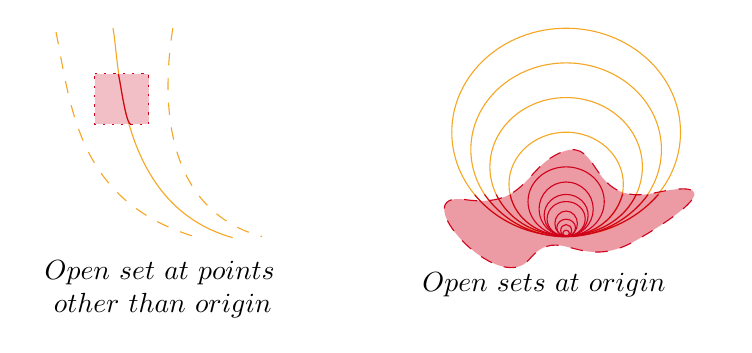
\begin{tikzpicture}[x=0.75pt,y=0.75pt,yscale=-1,xscale=1]
%uncomment if require: \path (0,300); %set diagram left start at 0, and has height of 300

%Flowchart: Connector [id:dp6190573425763748] 
\draw  [color={rgb, 255:red, 245; green, 166; blue, 35 }  ,draw opacity=1 ] (263.07,139.9) .. controls (263.07,112.23) and (287.74,89.8) .. (318.17,89.8) .. controls (348.6,89.8) and (373.27,112.23) .. (373.27,139.9) .. controls (373.27,167.57) and (348.6,190) .. (318.17,190) .. controls (287.74,190) and (263.07,167.57) .. (263.07,139.9) -- cycle ;
%Flowchart: Connector [id:dp7012306874990505] 
\draw  [color={rgb, 255:red, 245; green, 166; blue, 35 }  ,draw opacity=1 ] (272.25,148.25) .. controls (272.25,125.19) and (292.81,106.5) .. (318.17,106.5) .. controls (343.53,106.5) and (364.08,125.19) .. (364.08,148.25) .. controls (364.08,171.31) and (343.53,190) .. (318.17,190) .. controls (292.81,190) and (272.25,171.31) .. (272.25,148.25) -- cycle ;
%Flowchart: Connector [id:dp8115238254891972] 
\draw  [color={rgb, 255:red, 245; green, 166; blue, 35 }  ,draw opacity=1 ] (281.43,156.6) .. controls (281.43,138.15) and (297.88,123.2) .. (318.17,123.2) .. controls (338.45,123.2) and (354.9,138.15) .. (354.9,156.6) .. controls (354.9,175.05) and (338.45,190) .. (318.17,190) .. controls (297.88,190) and (281.43,175.05) .. (281.43,156.6) -- cycle ;
%Flowchart: Connector [id:dp13256721831630391] 
\draw  [color={rgb, 255:red, 245; green, 166; blue, 35 }  ,draw opacity=1 ] (290.62,164.95) .. controls (290.62,151.12) and (302.95,139.9) .. (318.17,139.9) .. controls (333.38,139.9) and (345.72,151.12) .. (345.72,164.95) .. controls (345.72,178.78) and (333.38,190) .. (318.17,190) .. controls (302.95,190) and (290.62,178.78) .. (290.62,164.95) -- cycle ;
%Flowchart: Connector [id:dp6922226533803466] 
\draw  [color={rgb, 255:red, 208; green, 2; blue, 27 }  ,draw opacity=1 ] (299.8,173.3) .. controls (299.8,164.08) and (308.02,156.6) .. (318.17,156.6) .. controls (328.31,156.6) and (336.53,164.08) .. (336.53,173.3) .. controls (336.53,182.52) and (328.31,190) .. (318.17,190) .. controls (308.02,190) and (299.8,182.52) .. (299.8,173.3) -- cycle ;
%Flowchart: Connector [id:dp24338136998325388] 
\draw  [color={rgb, 255:red, 208; green, 2; blue, 27 }  ,draw opacity=1 ] (308.98,181.65) .. controls (308.98,177.04) and (313.09,173.3) .. (318.17,173.3) .. controls (323.24,173.3) and (327.35,177.04) .. (327.35,181.65) .. controls (327.35,186.26) and (323.24,190) .. (318.17,190) .. controls (313.09,190) and (308.98,186.26) .. (308.98,181.65) -- cycle ;
%Flowchart: Connector [id:dp8937826625032416] 
\draw  [color={rgb, 255:red, 208; green, 2; blue, 27 }  ,draw opacity=1 ] (313.67,185.91) .. controls (313.67,183.65) and (315.68,181.82) .. (318.17,181.82) .. controls (320.65,181.82) and (322.67,183.65) .. (322.67,185.91) .. controls (322.67,188.17) and (320.65,190) .. (318.17,190) .. controls (315.68,190) and (313.67,188.17) .. (313.67,185.91) -- cycle ;
%Curve Lines [id:da4901637116911757] 
\draw [color={rgb, 255:red, 245; green, 166; blue, 35 }  ,draw opacity=1 ] [dash pattern={on 4.5pt off 4.5pt}]  (72.4,91.69) .. controls (79.96,129.88) and (83.27,174.67) .. (142.36,191.17) ;
%Curve Lines [id:da21170722213428972] 
\draw [color={rgb, 255:red, 245; green, 166; blue, 35 }  ,draw opacity=1 ]   (99.82,89.8) .. controls (103.13,106.3) and (101.71,175.14) .. (157.49,190.7) ;
%Curve Lines [id:da9517514166879361] 
\draw [color={rgb, 255:red, 245; green, 166; blue, 35 }  ,draw opacity=1 ] [dash pattern={on 4.5pt off 4.5pt}]  (128.65,89.8) .. controls (126.76,103) and (114.94,174.67) .. (171.67,190.22) ;
%Curve Lines [id:da7815842680204037] 
\draw [color={rgb, 255:red, 208; green, 2; blue, 27 }  ,draw opacity=1 ]   (102.25,112.03) .. controls (103.06,111.62) and (105.49,134.86) .. (108.33,136.07) ;
%Shape: Rectangle [id:dp3518891578525992] 
\draw  [color={rgb, 255:red, 208; green, 2; blue, 27 }  ,draw opacity=1 ][fill={rgb, 255:red, 208; green, 2; blue, 27 }  ,fill opacity=0.25 ][dash pattern={on 0.84pt off 2.51pt}] (91.11,111.62) -- (117.04,111.62) -- (117.04,136.07) -- (91.11,136.07) -- cycle ;
%Flowchart: Connector [id:dp8366596608471093] 
\draw  [color={rgb, 255:red, 208; green, 2; blue, 27 }  ,draw opacity=1 ] (315.54,187.19) .. controls (315.54,185.63) and (316.72,184.38) .. (318.17,184.38) .. controls (319.62,184.38) and (320.79,185.63) .. (320.79,187.19) .. controls (320.79,188.74) and (319.62,190) .. (318.17,190) .. controls (316.72,190) and (315.54,188.74) .. (315.54,187.19) -- cycle ;
%Flowchart: Connector [id:dp4493955981601927] 
\draw  [color={rgb, 255:red, 208; green, 2; blue, 27 }  ,draw opacity=1 ] (316.6,188.56) .. controls (316.6,187.77) and (317.3,187.13) .. (318.17,187.13) .. controls (319.03,187.13) and (319.73,187.77) .. (319.73,188.56) .. controls (319.73,189.36) and (319.03,190) .. (318.17,190) .. controls (317.3,190) and (316.6,189.36) .. (316.6,188.56) -- cycle ;
%Flowchart: Connector [id:dp19087752442781114] 
\draw  [color={rgb, 255:red, 208; green, 2; blue, 27 }  ,draw opacity=1 ] (312.73,183.94) .. controls (312.73,180.59) and (315.16,177.88) .. (318.17,177.88) .. controls (321.17,177.88) and (323.6,180.59) .. (323.6,183.94) .. controls (323.6,187.29) and (321.17,190) .. (318.17,190) .. controls (315.16,190) and (312.73,187.29) .. (312.73,183.94) -- cycle ;
%Flowchart: Connector [id:dp18742905436894852] 
\draw  [color={rgb, 255:red, 208; green, 2; blue, 27 }  ,draw opacity=1 ] (307.57,179.94) .. controls (307.57,174.38) and (312.32,169.88) .. (318.17,169.88) .. controls (324.02,169.88) and (328.76,174.38) .. (328.76,179.94) .. controls (328.76,185.49) and (324.02,190) .. (318.17,190) .. controls (312.32,190) and (307.57,185.49) .. (307.57,179.94) -- cycle ;
%Flowchart: Connector [id:dp4457066896455313] 
\draw  [color={rgb, 255:red, 208; green, 2; blue, 27 }  ,draw opacity=1 ] (305.12,176.94) .. controls (305.12,169.72) and (310.96,163.88) .. (318.17,163.88) .. controls (325.37,163.88) and (331.21,169.72) .. (331.21,176.94) .. controls (331.21,184.15) and (325.37,190) .. (318.17,190) .. controls (310.96,190) and (305.12,184.15) .. (305.12,176.94) -- cycle ;
%Curve Lines [id:da11974430372515932] 
\draw [color={rgb, 255:red, 208; green, 2; blue, 27 }  ,draw opacity=1 ]   (291.14,169.95) .. controls (296.84,195.02) and (337.04,197.84) .. (345.46,169.63) ;
%Curve Lines [id:da6813221748543254] 
\draw [color={rgb, 255:red, 208; green, 2; blue, 27 }  ,draw opacity=1 ]   (284.51,169.95) .. controls (297.98,197.42) and (340.61,195.11) .. (351.98,169.74) ;
%Curve Lines [id:da1609800887372339] 
\draw [color={rgb, 255:red, 208; green, 2; blue, 27 }  ,draw opacity=1 ]   (278.84,169.91) .. controls (299.46,198.26) and (338.3,195.84) .. (357.56,170.05) ;
%Curve Lines [id:da478917001221287] 
\draw [color={rgb, 255:red, 208; green, 2; blue, 27 }  ,draw opacity=1 ]   (274.1,170.02) .. controls (295.46,196.26) and (338.82,196.89) .. (362.61,169.95) ;
%Shape: Polygon Curved [id:ds09761740084492965] 
\draw  [color={rgb, 255:red, 208; green, 2; blue, 27 }  ,draw opacity=1 ][fill={rgb, 255:red, 208; green, 2; blue, 27 }  ,fill opacity=0.4 ][dash pattern={on 4.5pt off 4.5pt}] (269.46,172.36) .. controls (299.6,176.8) and (298,156.25) .. (316.67,149.25) .. controls (335.33,142.25) and (328.67,176.08) .. (361.17,169.08) .. controls (393.67,162.08) and (379.76,175.81) .. (352,191.92) .. controls (324.24,208.03) and (315.5,183.08) .. (300.33,201.25) .. controls (285.17,219.42) and (239.33,167.92) .. (269.46,172.36) -- cycle ;

% Text Node
\draw (59,198.4) node [anchor=north west][inner sep=0.75pt]    {$ \begin{array}{l}
Open\ set\ at\ points\ \\
\ other\ than\ origin
\end{array}$};
% Text Node
\draw (247.67,206.07) node [anchor=north west][inner sep=0.75pt]    {$Open\ sets\ at\ origin$};


\end{tikzpicture}


    \end{center}
\end{frame}


\framecard[colorgreen]{{\color{white}\hugetext{Construction of $Y$ and $Z$}}}

\begin{frame}{Construction of $Y$}
    Define \textcolor{colororange}{$\tilde H=\bigcup_{i=2}^n C_i$}. $\tilde H$ is like the Hawaiian earring with the outemost shell removed. Define: \textcolor{colororange}{$$Y=\left(\bigcup_{z\in\mathbb Z}(z+\tilde H)\right)\cup\mathbb R$$}\pause which looks likes the following
    \begin{center}
        


\tikzset{every picture/.style={line width=0.75pt}} %set default line width to 0.75pt        

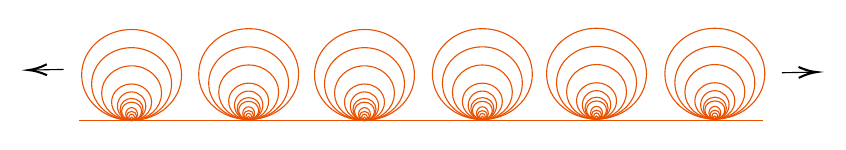
\begin{tikzpicture}[x=0.6pt,y=0.6pt,yscale=-1,xscale=1]
%uncomment if require: \path (0,300); %set diagram left start at 0, and has height of 300

%Flowchart: Connector [id:dp6118635117969007] 
\draw  [color={rgb, 255:red, 233; green, 81; blue, 0 }  ,draw opacity=1 ] (90.08,172.3) .. controls (90.08,157.19) and (103.55,144.94) .. (120.17,144.94) .. controls (136.78,144.94) and (150.25,157.19) .. (150.25,172.3) .. controls (150.25,187.4) and (136.78,199.65) .. (120.17,199.65) .. controls (103.55,199.65) and (90.08,187.4) .. (90.08,172.3) -- cycle ;
%Flowchart: Connector [id:dp021286863927374222] 
\draw  [color={rgb, 255:red, 233; green, 81; blue, 0 }  ,draw opacity=1 ] (96.1,177.77) .. controls (96.1,165.68) and (106.88,155.89) .. (120.17,155.89) .. controls (133.46,155.89) and (144.23,165.68) .. (144.23,177.77) .. controls (144.23,189.85) and (133.46,199.65) .. (120.17,199.65) .. controls (106.88,199.65) and (96.1,189.85) .. (96.1,177.77) -- cycle ;
%Flowchart: Connector [id:dp2527774079894154] 
\draw  [color={rgb, 255:red, 233; green, 81; blue, 0 }  ,draw opacity=1 ] (102.12,183.24) .. controls (102.12,174.17) and (110.2,166.83) .. (120.17,166.83) .. controls (130.14,166.83) and (138.22,174.17) .. (138.22,183.24) .. controls (138.22,192.3) and (130.14,199.65) .. (120.17,199.65) .. controls (110.2,199.65) and (102.12,192.3) .. (102.12,183.24) -- cycle ;
%Flowchart: Connector [id:dp08417943975806563] 
\draw  [color={rgb, 255:red, 233; green, 81; blue, 0 }  ,draw opacity=1 ] (108.13,188.71) .. controls (108.13,182.67) and (113.52,177.77) .. (120.17,177.77) .. controls (126.81,177.77) and (132.2,182.67) .. (132.2,188.71) .. controls (132.2,194.75) and (126.81,199.65) .. (120.17,199.65) .. controls (113.52,199.65) and (108.13,194.75) .. (108.13,188.71) -- cycle ;
%Flowchart: Connector [id:dp29414523801430925] 
\draw  [color={rgb, 255:red, 233; green, 81; blue, 0 }  ,draw opacity=1 ] (114.15,194.18) .. controls (114.15,191.16) and (116.84,188.71) .. (120.17,188.71) .. controls (123.49,188.71) and (126.18,191.16) .. (126.18,194.18) .. controls (126.18,197.2) and (123.49,199.65) .. (120.17,199.65) .. controls (116.84,199.65) and (114.15,197.2) .. (114.15,194.18) -- cycle ;
%Flowchart: Connector [id:dp029098174271795396] 
\draw  [color={rgb, 255:red, 233; green, 81; blue, 0 }  ,draw opacity=1 ] (117.22,196.97) .. controls (117.22,195.49) and (118.54,194.29) .. (120.17,194.29) .. controls (121.79,194.29) and (123.11,195.49) .. (123.11,196.97) .. controls (123.11,198.45) and (121.79,199.65) .. (120.17,199.65) .. controls (118.54,199.65) and (117.22,198.45) .. (117.22,196.97) -- cycle ;
%Flowchart: Connector [id:dp6415676425954105] 
\draw  [color={rgb, 255:red, 233; green, 81; blue, 0 }  ,draw opacity=1 ] (118.45,197.81) .. controls (118.45,196.79) and (119.22,195.97) .. (120.17,195.97) .. controls (121.12,195.97) and (121.89,196.79) .. (121.89,197.81) .. controls (121.89,198.83) and (121.12,199.65) .. (120.17,199.65) .. controls (119.22,199.65) and (118.45,198.83) .. (118.45,197.81) -- cycle ;
%Flowchart: Connector [id:dp17774482388157442] 
\draw  [color={rgb, 255:red, 233; green, 81; blue, 0 }  ,draw opacity=1 ] (119.14,198.71) .. controls (119.14,198.19) and (119.6,197.77) .. (120.17,197.77) .. controls (120.73,197.77) and (121.19,198.19) .. (121.19,198.71) .. controls (121.19,199.23) and (120.73,199.65) .. (120.17,199.65) .. controls (119.6,199.65) and (119.14,199.23) .. (119.14,198.71) -- cycle ;
%Flowchart: Connector [id:dp06615937323137455] 
\draw  [color={rgb, 255:red, 233; green, 81; blue, 0 }  ,draw opacity=1 ] (116.6,195.97) .. controls (116.6,193.77) and (118.2,191.99) .. (120.17,191.99) .. controls (122.13,191.99) and (123.73,193.77) .. (123.73,195.97) .. controls (123.73,198.16) and (122.13,199.94) .. (120.17,199.94) .. controls (118.2,199.94) and (116.6,198.16) .. (116.6,195.97) -- cycle ;
%Flowchart: Connector [id:dp5327366929429374] 
\draw  [color={rgb, 255:red, 233; green, 81; blue, 0 }  ,draw opacity=1 ] (113.23,193.06) .. controls (113.23,189.42) and (116.33,186.47) .. (120.17,186.47) .. controls (124,186.47) and (127.11,189.42) .. (127.11,193.06) .. controls (127.11,196.7) and (124,199.65) .. (120.17,199.65) .. controls (116.33,199.65) and (113.23,196.7) .. (113.23,193.06) -- cycle ;
%Flowchart: Connector [id:dp5051267191158141] 
\draw  [color={rgb, 255:red, 233; green, 81; blue, 0 }  ,draw opacity=1 ] (111.62,191.09) .. controls (111.62,186.37) and (115.45,182.53) .. (120.17,182.53) .. controls (124.89,182.53) and (128.71,186.37) .. (128.71,191.09) .. controls (128.71,195.82) and (124.89,199.65) .. (120.17,199.65) .. controls (115.45,199.65) and (111.62,195.82) .. (111.62,191.09) -- cycle ;

%Straight Lines [id:da4779609215734192] 
\draw [color={rgb, 255:red, 233; green, 81; blue, 0 }  ,draw opacity=1 ]   (88.67,199.83) -- (500.33,199.83) ;
%Flowchart: Connector [id:dp5213839523733965] 
\draw  [color={rgb, 255:red, 233; green, 81; blue, 0 }  ,draw opacity=1 ] (160.58,171.8) .. controls (160.58,156.69) and (174.05,144.44) .. (190.67,144.44) .. controls (207.28,144.44) and (220.75,156.69) .. (220.75,171.8) .. controls (220.75,186.9) and (207.28,199.15) .. (190.67,199.15) .. controls (174.05,199.15) and (160.58,186.9) .. (160.58,171.8) -- cycle ;
%Flowchart: Connector [id:dp7147792085745278] 
\draw  [color={rgb, 255:red, 233; green, 81; blue, 0 }  ,draw opacity=1 ] (166.6,177.27) .. controls (166.6,165.18) and (177.38,155.39) .. (190.67,155.39) .. controls (203.96,155.39) and (214.73,165.18) .. (214.73,177.27) .. controls (214.73,189.35) and (203.96,199.15) .. (190.67,199.15) .. controls (177.38,199.15) and (166.6,189.35) .. (166.6,177.27) -- cycle ;
%Flowchart: Connector [id:dp7861143744371363] 
\draw  [color={rgb, 255:red, 233; green, 81; blue, 0 }  ,draw opacity=1 ] (172.62,182.74) .. controls (172.62,173.67) and (180.7,166.33) .. (190.67,166.33) .. controls (200.64,166.33) and (208.72,173.67) .. (208.72,182.74) .. controls (208.72,191.8) and (200.64,199.15) .. (190.67,199.15) .. controls (180.7,199.15) and (172.62,191.8) .. (172.62,182.74) -- cycle ;
%Flowchart: Connector [id:dp488931432460622] 
\draw  [color={rgb, 255:red, 233; green, 81; blue, 0 }  ,draw opacity=1 ] (178.63,188.21) .. controls (178.63,182.17) and (184.02,177.27) .. (190.67,177.27) .. controls (197.31,177.27) and (202.7,182.17) .. (202.7,188.21) .. controls (202.7,194.25) and (197.31,199.15) .. (190.67,199.15) .. controls (184.02,199.15) and (178.63,194.25) .. (178.63,188.21) -- cycle ;
%Flowchart: Connector [id:dp39724012685478616] 
\draw  [color={rgb, 255:red, 233; green, 81; blue, 0 }  ,draw opacity=1 ] (184.65,193.68) .. controls (184.65,190.66) and (187.34,188.21) .. (190.67,188.21) .. controls (193.99,188.21) and (196.68,190.66) .. (196.68,193.68) .. controls (196.68,196.7) and (193.99,199.15) .. (190.67,199.15) .. controls (187.34,199.15) and (184.65,196.7) .. (184.65,193.68) -- cycle ;
%Flowchart: Connector [id:dp04224686297953417] 
\draw  [color={rgb, 255:red, 233; green, 81; blue, 0 }  ,draw opacity=1 ] (187.72,196.47) .. controls (187.72,194.99) and (189.04,193.79) .. (190.67,193.79) .. controls (192.29,193.79) and (193.61,194.99) .. (193.61,196.47) .. controls (193.61,197.95) and (192.29,199.15) .. (190.67,199.15) .. controls (189.04,199.15) and (187.72,197.95) .. (187.72,196.47) -- cycle ;
%Flowchart: Connector [id:dp8473928946525451] 
\draw  [color={rgb, 255:red, 233; green, 81; blue, 0 }  ,draw opacity=1 ] (188.95,197.31) .. controls (188.95,196.29) and (189.72,195.47) .. (190.67,195.47) .. controls (191.62,195.47) and (192.39,196.29) .. (192.39,197.31) .. controls (192.39,198.33) and (191.62,199.15) .. (190.67,199.15) .. controls (189.72,199.15) and (188.95,198.33) .. (188.95,197.31) -- cycle ;
%Flowchart: Connector [id:dp16869614585014747] 
\draw  [color={rgb, 255:red, 233; green, 81; blue, 0 }  ,draw opacity=1 ] (189.64,198.21) .. controls (189.64,197.69) and (190.1,197.27) .. (190.67,197.27) .. controls (191.23,197.27) and (191.69,197.69) .. (191.69,198.21) .. controls (191.69,198.73) and (191.23,199.15) .. (190.67,199.15) .. controls (190.1,199.15) and (189.64,198.73) .. (189.64,198.21) -- cycle ;
%Flowchart: Connector [id:dp13717248030857587] 
\draw  [color={rgb, 255:red, 233; green, 81; blue, 0 }  ,draw opacity=1 ] (187.1,195.47) .. controls (187.1,193.27) and (188.7,191.49) .. (190.67,191.49) .. controls (192.63,191.49) and (194.23,193.27) .. (194.23,195.47) .. controls (194.23,197.66) and (192.63,199.44) .. (190.67,199.44) .. controls (188.7,199.44) and (187.1,197.66) .. (187.1,195.47) -- cycle ;
%Flowchart: Connector [id:dp7945334411173829] 
\draw  [color={rgb, 255:red, 233; green, 81; blue, 0 }  ,draw opacity=1 ] (183.73,192.56) .. controls (183.73,188.92) and (186.83,185.97) .. (190.67,185.97) .. controls (194.5,185.97) and (197.61,188.92) .. (197.61,192.56) .. controls (197.61,196.2) and (194.5,199.15) .. (190.67,199.15) .. controls (186.83,199.15) and (183.73,196.2) .. (183.73,192.56) -- cycle ;
%Flowchart: Connector [id:dp8661145219284314] 
\draw  [color={rgb, 255:red, 233; green, 81; blue, 0 }  ,draw opacity=1 ] (182.12,190.59) .. controls (182.12,185.87) and (185.95,182.03) .. (190.67,182.03) .. controls (195.39,182.03) and (199.21,185.87) .. (199.21,190.59) .. controls (199.21,195.32) and (195.39,199.15) .. (190.67,199.15) .. controls (185.95,199.15) and (182.12,195.32) .. (182.12,190.59) -- cycle ;

%Flowchart: Connector [id:dp08990553053002448] 
\draw  [color={rgb, 255:red, 233; green, 81; blue, 0 }  ,draw opacity=1 ] (230.33,172.3) .. controls (230.33,157.19) and (243.8,144.94) .. (260.42,144.94) .. controls (277.03,144.94) and (290.5,157.19) .. (290.5,172.3) .. controls (290.5,187.4) and (277.03,199.65) .. (260.42,199.65) .. controls (243.8,199.65) and (230.33,187.4) .. (230.33,172.3) -- cycle ;
%Flowchart: Connector [id:dp9680065196342099] 
\draw  [color={rgb, 255:red, 233; green, 81; blue, 0 }  ,draw opacity=1 ] (236.35,177.77) .. controls (236.35,165.68) and (247.13,155.89) .. (260.42,155.89) .. controls (273.71,155.89) and (284.48,165.68) .. (284.48,177.77) .. controls (284.48,189.85) and (273.71,199.65) .. (260.42,199.65) .. controls (247.13,199.65) and (236.35,189.85) .. (236.35,177.77) -- cycle ;
%Flowchart: Connector [id:dp6156719861278815] 
\draw  [color={rgb, 255:red, 233; green, 81; blue, 0 }  ,draw opacity=1 ] (242.37,183.24) .. controls (242.37,174.17) and (250.45,166.83) .. (260.42,166.83) .. controls (270.39,166.83) and (278.47,174.17) .. (278.47,183.24) .. controls (278.47,192.3) and (270.39,199.65) .. (260.42,199.65) .. controls (250.45,199.65) and (242.37,192.3) .. (242.37,183.24) -- cycle ;
%Flowchart: Connector [id:dp9161709993762697] 
\draw  [color={rgb, 255:red, 233; green, 81; blue, 0 }  ,draw opacity=1 ] (248.38,188.71) .. controls (248.38,182.67) and (253.77,177.77) .. (260.42,177.77) .. controls (267.06,177.77) and (272.45,182.67) .. (272.45,188.71) .. controls (272.45,194.75) and (267.06,199.65) .. (260.42,199.65) .. controls (253.77,199.65) and (248.38,194.75) .. (248.38,188.71) -- cycle ;
%Flowchart: Connector [id:dp5030407893811631] 
\draw  [color={rgb, 255:red, 233; green, 81; blue, 0 }  ,draw opacity=1 ] (254.4,194.18) .. controls (254.4,191.16) and (257.09,188.71) .. (260.42,188.71) .. controls (263.74,188.71) and (266.43,191.16) .. (266.43,194.18) .. controls (266.43,197.2) and (263.74,199.65) .. (260.42,199.65) .. controls (257.09,199.65) and (254.4,197.2) .. (254.4,194.18) -- cycle ;
%Flowchart: Connector [id:dp19761145493465737] 
\draw  [color={rgb, 255:red, 233; green, 81; blue, 0 }  ,draw opacity=1 ] (257.47,196.97) .. controls (257.47,195.49) and (258.79,194.29) .. (260.42,194.29) .. controls (262.04,194.29) and (263.36,195.49) .. (263.36,196.97) .. controls (263.36,198.45) and (262.04,199.65) .. (260.42,199.65) .. controls (258.79,199.65) and (257.47,198.45) .. (257.47,196.97) -- cycle ;
%Flowchart: Connector [id:dp6771102729547135] 
\draw  [color={rgb, 255:red, 233; green, 81; blue, 0 }  ,draw opacity=1 ] (258.7,197.81) .. controls (258.7,196.79) and (259.47,195.97) .. (260.42,195.97) .. controls (261.37,195.97) and (262.14,196.79) .. (262.14,197.81) .. controls (262.14,198.83) and (261.37,199.65) .. (260.42,199.65) .. controls (259.47,199.65) and (258.7,198.83) .. (258.7,197.81) -- cycle ;
%Flowchart: Connector [id:dp45574110219141906] 
\draw  [color={rgb, 255:red, 233; green, 81; blue, 0 }  ,draw opacity=1 ] (259.39,198.71) .. controls (259.39,198.19) and (259.85,197.77) .. (260.42,197.77) .. controls (260.98,197.77) and (261.44,198.19) .. (261.44,198.71) .. controls (261.44,199.23) and (260.98,199.65) .. (260.42,199.65) .. controls (259.85,199.65) and (259.39,199.23) .. (259.39,198.71) -- cycle ;
%Flowchart: Connector [id:dp17401793828716272] 
\draw  [color={rgb, 255:red, 233; green, 81; blue, 0 }  ,draw opacity=1 ] (256.85,195.97) .. controls (256.85,193.77) and (258.45,191.99) .. (260.42,191.99) .. controls (262.38,191.99) and (263.98,193.77) .. (263.98,195.97) .. controls (263.98,198.16) and (262.38,199.94) .. (260.42,199.94) .. controls (258.45,199.94) and (256.85,198.16) .. (256.85,195.97) -- cycle ;
%Flowchart: Connector [id:dp8695900065688762] 
\draw  [color={rgb, 255:red, 233; green, 81; blue, 0 }  ,draw opacity=1 ] (253.48,193.06) .. controls (253.48,189.42) and (256.58,186.47) .. (260.42,186.47) .. controls (264.25,186.47) and (267.36,189.42) .. (267.36,193.06) .. controls (267.36,196.7) and (264.25,199.65) .. (260.42,199.65) .. controls (256.58,199.65) and (253.48,196.7) .. (253.48,193.06) -- cycle ;
%Flowchart: Connector [id:dp41517076055941826] 
\draw  [color={rgb, 255:red, 233; green, 81; blue, 0 }  ,draw opacity=1 ] (251.87,191.09) .. controls (251.87,186.37) and (255.7,182.53) .. (260.42,182.53) .. controls (265.14,182.53) and (268.96,186.37) .. (268.96,191.09) .. controls (268.96,195.82) and (265.14,199.65) .. (260.42,199.65) .. controls (255.7,199.65) and (251.87,195.82) .. (251.87,191.09) -- cycle ;

%Flowchart: Connector [id:dp07854222033930713] 
\draw  [color={rgb, 255:red, 233; green, 81; blue, 0 }  ,draw opacity=1 ] (301.33,171.8) .. controls (301.33,156.69) and (314.8,144.44) .. (331.42,144.44) .. controls (348.03,144.44) and (361.5,156.69) .. (361.5,171.8) .. controls (361.5,186.9) and (348.03,199.15) .. (331.42,199.15) .. controls (314.8,199.15) and (301.33,186.9) .. (301.33,171.8) -- cycle ;
%Flowchart: Connector [id:dp12436186076650235] 
\draw  [color={rgb, 255:red, 233; green, 81; blue, 0 }  ,draw opacity=1 ] (307.35,177.27) .. controls (307.35,165.18) and (318.13,155.39) .. (331.42,155.39) .. controls (344.71,155.39) and (355.48,165.18) .. (355.48,177.27) .. controls (355.48,189.35) and (344.71,199.15) .. (331.42,199.15) .. controls (318.13,199.15) and (307.35,189.35) .. (307.35,177.27) -- cycle ;
%Flowchart: Connector [id:dp9027674612810805] 
\draw  [color={rgb, 255:red, 233; green, 81; blue, 0 }  ,draw opacity=1 ] (313.37,182.74) .. controls (313.37,173.67) and (321.45,166.33) .. (331.42,166.33) .. controls (341.39,166.33) and (349.47,173.67) .. (349.47,182.74) .. controls (349.47,191.8) and (341.39,199.15) .. (331.42,199.15) .. controls (321.45,199.15) and (313.37,191.8) .. (313.37,182.74) -- cycle ;
%Flowchart: Connector [id:dp6458513898415574] 
\draw  [color={rgb, 255:red, 233; green, 81; blue, 0 }  ,draw opacity=1 ] (319.38,188.21) .. controls (319.38,182.17) and (324.77,177.27) .. (331.42,177.27) .. controls (338.06,177.27) and (343.45,182.17) .. (343.45,188.21) .. controls (343.45,194.25) and (338.06,199.15) .. (331.42,199.15) .. controls (324.77,199.15) and (319.38,194.25) .. (319.38,188.21) -- cycle ;
%Flowchart: Connector [id:dp9610835700416278] 
\draw  [color={rgb, 255:red, 233; green, 81; blue, 0 }  ,draw opacity=1 ] (325.4,193.68) .. controls (325.4,190.66) and (328.09,188.21) .. (331.42,188.21) .. controls (334.74,188.21) and (337.43,190.66) .. (337.43,193.68) .. controls (337.43,196.7) and (334.74,199.15) .. (331.42,199.15) .. controls (328.09,199.15) and (325.4,196.7) .. (325.4,193.68) -- cycle ;
%Flowchart: Connector [id:dp2012923446813779] 
\draw  [color={rgb, 255:red, 233; green, 81; blue, 0 }  ,draw opacity=1 ] (328.47,196.47) .. controls (328.47,194.99) and (329.79,193.79) .. (331.42,193.79) .. controls (333.04,193.79) and (334.36,194.99) .. (334.36,196.47) .. controls (334.36,197.95) and (333.04,199.15) .. (331.42,199.15) .. controls (329.79,199.15) and (328.47,197.95) .. (328.47,196.47) -- cycle ;
%Flowchart: Connector [id:dp31470603940034003] 
\draw  [color={rgb, 255:red, 233; green, 81; blue, 0 }  ,draw opacity=1 ] (329.7,197.31) .. controls (329.7,196.29) and (330.47,195.47) .. (331.42,195.47) .. controls (332.37,195.47) and (333.14,196.29) .. (333.14,197.31) .. controls (333.14,198.33) and (332.37,199.15) .. (331.42,199.15) .. controls (330.47,199.15) and (329.7,198.33) .. (329.7,197.31) -- cycle ;
%Flowchart: Connector [id:dp6990958765312496] 
\draw  [color={rgb, 255:red, 233; green, 81; blue, 0 }  ,draw opacity=1 ] (330.39,198.21) .. controls (330.39,197.69) and (330.85,197.27) .. (331.42,197.27) .. controls (331.98,197.27) and (332.44,197.69) .. (332.44,198.21) .. controls (332.44,198.73) and (331.98,199.15) .. (331.42,199.15) .. controls (330.85,199.15) and (330.39,198.73) .. (330.39,198.21) -- cycle ;
%Flowchart: Connector [id:dp7312310665614428] 
\draw  [color={rgb, 255:red, 233; green, 81; blue, 0 }  ,draw opacity=1 ] (327.85,195.47) .. controls (327.85,193.27) and (329.45,191.49) .. (331.42,191.49) .. controls (333.38,191.49) and (334.98,193.27) .. (334.98,195.47) .. controls (334.98,197.66) and (333.38,199.44) .. (331.42,199.44) .. controls (329.45,199.44) and (327.85,197.66) .. (327.85,195.47) -- cycle ;
%Flowchart: Connector [id:dp22281789521827622] 
\draw  [color={rgb, 255:red, 233; green, 81; blue, 0 }  ,draw opacity=1 ] (324.48,192.56) .. controls (324.48,188.92) and (327.58,185.97) .. (331.42,185.97) .. controls (335.25,185.97) and (338.36,188.92) .. (338.36,192.56) .. controls (338.36,196.2) and (335.25,199.15) .. (331.42,199.15) .. controls (327.58,199.15) and (324.48,196.2) .. (324.48,192.56) -- cycle ;
%Flowchart: Connector [id:dp19742973064027447] 
\draw  [color={rgb, 255:red, 233; green, 81; blue, 0 }  ,draw opacity=1 ] (322.87,190.59) .. controls (322.87,185.87) and (326.7,182.03) .. (331.42,182.03) .. controls (336.14,182.03) and (339.96,185.87) .. (339.96,190.59) .. controls (339.96,195.32) and (336.14,199.15) .. (331.42,199.15) .. controls (326.7,199.15) and (322.87,195.32) .. (322.87,190.59) -- cycle ;

%Flowchart: Connector [id:dp509084746160488] 
\draw  [color={rgb, 255:red, 233; green, 81; blue, 0 }  ,draw opacity=1 ] (370.08,171.55) .. controls (370.08,156.44) and (383.55,144.19) .. (400.17,144.19) .. controls (416.78,144.19) and (430.25,156.44) .. (430.25,171.55) .. controls (430.25,186.65) and (416.78,198.9) .. (400.17,198.9) .. controls (383.55,198.9) and (370.08,186.65) .. (370.08,171.55) -- cycle ;
%Flowchart: Connector [id:dp02115403752748035] 
\draw  [color={rgb, 255:red, 233; green, 81; blue, 0 }  ,draw opacity=1 ] (376.1,177.02) .. controls (376.1,164.93) and (386.88,155.14) .. (400.17,155.14) .. controls (413.46,155.14) and (424.23,164.93) .. (424.23,177.02) .. controls (424.23,189.1) and (413.46,198.9) .. (400.17,198.9) .. controls (386.88,198.9) and (376.1,189.1) .. (376.1,177.02) -- cycle ;
%Flowchart: Connector [id:dp1421853599060139] 
\draw  [color={rgb, 255:red, 233; green, 81; blue, 0 }  ,draw opacity=1 ] (382.12,182.49) .. controls (382.12,173.42) and (390.2,166.08) .. (400.17,166.08) .. controls (410.14,166.08) and (418.22,173.42) .. (418.22,182.49) .. controls (418.22,191.55) and (410.14,198.9) .. (400.17,198.9) .. controls (390.2,198.9) and (382.12,191.55) .. (382.12,182.49) -- cycle ;
%Flowchart: Connector [id:dp17821891751971253] 
\draw  [color={rgb, 255:red, 233; green, 81; blue, 0 }  ,draw opacity=1 ] (388.13,187.96) .. controls (388.13,181.92) and (393.52,177.02) .. (400.17,177.02) .. controls (406.81,177.02) and (412.2,181.92) .. (412.2,187.96) .. controls (412.2,194) and (406.81,198.9) .. (400.17,198.9) .. controls (393.52,198.9) and (388.13,194) .. (388.13,187.96) -- cycle ;
%Flowchart: Connector [id:dp7774363729546013] 
\draw  [color={rgb, 255:red, 233; green, 81; blue, 0 }  ,draw opacity=1 ] (394.15,193.43) .. controls (394.15,190.41) and (396.84,187.96) .. (400.17,187.96) .. controls (403.49,187.96) and (406.18,190.41) .. (406.18,193.43) .. controls (406.18,196.45) and (403.49,198.9) .. (400.17,198.9) .. controls (396.84,198.9) and (394.15,196.45) .. (394.15,193.43) -- cycle ;
%Flowchart: Connector [id:dp523574326008853] 
\draw  [color={rgb, 255:red, 233; green, 81; blue, 0 }  ,draw opacity=1 ] (397.22,196.22) .. controls (397.22,194.74) and (398.54,193.54) .. (400.17,193.54) .. controls (401.79,193.54) and (403.11,194.74) .. (403.11,196.22) .. controls (403.11,197.7) and (401.79,198.9) .. (400.17,198.9) .. controls (398.54,198.9) and (397.22,197.7) .. (397.22,196.22) -- cycle ;
%Flowchart: Connector [id:dp7567047545223234] 
\draw  [color={rgb, 255:red, 233; green, 81; blue, 0 }  ,draw opacity=1 ] (398.45,197.06) .. controls (398.45,196.04) and (399.22,195.22) .. (400.17,195.22) .. controls (401.12,195.22) and (401.89,196.04) .. (401.89,197.06) .. controls (401.89,198.08) and (401.12,198.9) .. (400.17,198.9) .. controls (399.22,198.9) and (398.45,198.08) .. (398.45,197.06) -- cycle ;
%Flowchart: Connector [id:dp9522588519454986] 
\draw  [color={rgb, 255:red, 233; green, 81; blue, 0 }  ,draw opacity=1 ] (399.14,197.96) .. controls (399.14,197.44) and (399.6,197.02) .. (400.17,197.02) .. controls (400.73,197.02) and (401.19,197.44) .. (401.19,197.96) .. controls (401.19,198.48) and (400.73,198.9) .. (400.17,198.9) .. controls (399.6,198.9) and (399.14,198.48) .. (399.14,197.96) -- cycle ;
%Flowchart: Connector [id:dp7586926370196964] 
\draw  [color={rgb, 255:red, 233; green, 81; blue, 0 }  ,draw opacity=1 ] (396.6,195.22) .. controls (396.6,193.02) and (398.2,191.24) .. (400.17,191.24) .. controls (402.13,191.24) and (403.73,193.02) .. (403.73,195.22) .. controls (403.73,197.41) and (402.13,199.19) .. (400.17,199.19) .. controls (398.2,199.19) and (396.6,197.41) .. (396.6,195.22) -- cycle ;
%Flowchart: Connector [id:dp06377905142128615] 
\draw  [color={rgb, 255:red, 233; green, 81; blue, 0 }  ,draw opacity=1 ] (393.23,192.31) .. controls (393.23,188.67) and (396.33,185.72) .. (400.17,185.72) .. controls (404,185.72) and (407.11,188.67) .. (407.11,192.31) .. controls (407.11,195.95) and (404,198.9) .. (400.17,198.9) .. controls (396.33,198.9) and (393.23,195.95) .. (393.23,192.31) -- cycle ;
%Flowchart: Connector [id:dp1823603288937088] 
\draw  [color={rgb, 255:red, 233; green, 81; blue, 0 }  ,draw opacity=1 ] (391.62,190.34) .. controls (391.62,185.62) and (395.45,181.78) .. (400.17,181.78) .. controls (404.89,181.78) and (408.71,185.62) .. (408.71,190.34) .. controls (408.71,195.07) and (404.89,198.9) .. (400.17,198.9) .. controls (395.45,198.9) and (391.62,195.07) .. (391.62,190.34) -- cycle ;

%Flowchart: Connector [id:dp8629335848862278] 
\draw  [color={rgb, 255:red, 233; green, 81; blue, 0 }  ,draw opacity=1 ] (441.33,171.55) .. controls (441.33,156.44) and (454.8,144.19) .. (471.42,144.19) .. controls (488.03,144.19) and (501.5,156.44) .. (501.5,171.55) .. controls (501.5,186.65) and (488.03,198.9) .. (471.42,198.9) .. controls (454.8,198.9) and (441.33,186.65) .. (441.33,171.55) -- cycle ;
%Flowchart: Connector [id:dp9295833219743496] 
\draw  [color={rgb, 255:red, 233; green, 81; blue, 0 }  ,draw opacity=1 ] (447.35,177.02) .. controls (447.35,164.93) and (458.13,155.14) .. (471.42,155.14) .. controls (484.71,155.14) and (495.48,164.93) .. (495.48,177.02) .. controls (495.48,189.1) and (484.71,198.9) .. (471.42,198.9) .. controls (458.13,198.9) and (447.35,189.1) .. (447.35,177.02) -- cycle ;
%Flowchart: Connector [id:dp6324022103914927] 
\draw  [color={rgb, 255:red, 233; green, 81; blue, 0 }  ,draw opacity=1 ] (453.37,182.49) .. controls (453.37,173.42) and (461.45,166.08) .. (471.42,166.08) .. controls (481.39,166.08) and (489.47,173.42) .. (489.47,182.49) .. controls (489.47,191.55) and (481.39,198.9) .. (471.42,198.9) .. controls (461.45,198.9) and (453.37,191.55) .. (453.37,182.49) -- cycle ;
%Flowchart: Connector [id:dp6312163285056566] 
\draw  [color={rgb, 255:red, 233; green, 81; blue, 0 }  ,draw opacity=1 ] (459.38,187.96) .. controls (459.38,181.92) and (464.77,177.02) .. (471.42,177.02) .. controls (478.06,177.02) and (483.45,181.92) .. (483.45,187.96) .. controls (483.45,194) and (478.06,198.9) .. (471.42,198.9) .. controls (464.77,198.9) and (459.38,194) .. (459.38,187.96) -- cycle ;
%Flowchart: Connector [id:dp02057873879073613] 
\draw  [color={rgb, 255:red, 233; green, 81; blue, 0 }  ,draw opacity=1 ] (465.4,193.43) .. controls (465.4,190.41) and (468.09,187.96) .. (471.42,187.96) .. controls (474.74,187.96) and (477.43,190.41) .. (477.43,193.43) .. controls (477.43,196.45) and (474.74,198.9) .. (471.42,198.9) .. controls (468.09,198.9) and (465.4,196.45) .. (465.4,193.43) -- cycle ;
%Flowchart: Connector [id:dp233954444950618] 
\draw  [color={rgb, 255:red, 233; green, 81; blue, 0 }  ,draw opacity=1 ] (468.47,196.22) .. controls (468.47,194.74) and (469.79,193.54) .. (471.42,193.54) .. controls (473.04,193.54) and (474.36,194.74) .. (474.36,196.22) .. controls (474.36,197.7) and (473.04,198.9) .. (471.42,198.9) .. controls (469.79,198.9) and (468.47,197.7) .. (468.47,196.22) -- cycle ;
%Flowchart: Connector [id:dp2504097896948497] 
\draw  [color={rgb, 255:red, 233; green, 81; blue, 0 }  ,draw opacity=1 ] (469.7,197.06) .. controls (469.7,196.04) and (470.47,195.22) .. (471.42,195.22) .. controls (472.37,195.22) and (473.14,196.04) .. (473.14,197.06) .. controls (473.14,198.08) and (472.37,198.9) .. (471.42,198.9) .. controls (470.47,198.9) and (469.7,198.08) .. (469.7,197.06) -- cycle ;
%Flowchart: Connector [id:dp39675294025492747] 
\draw  [color={rgb, 255:red, 233; green, 81; blue, 0 }  ,draw opacity=1 ] (470.39,197.96) .. controls (470.39,197.44) and (470.85,197.02) .. (471.42,197.02) .. controls (471.98,197.02) and (472.44,197.44) .. (472.44,197.96) .. controls (472.44,198.48) and (471.98,198.9) .. (471.42,198.9) .. controls (470.85,198.9) and (470.39,198.48) .. (470.39,197.96) -- cycle ;
%Flowchart: Connector [id:dp8297923399476581] 
\draw  [color={rgb, 255:red, 233; green, 81; blue, 0 }  ,draw opacity=1 ] (467.85,195.22) .. controls (467.85,193.02) and (469.45,191.24) .. (471.42,191.24) .. controls (473.38,191.24) and (474.98,193.02) .. (474.98,195.22) .. controls (474.98,197.41) and (473.38,199.19) .. (471.42,199.19) .. controls (469.45,199.19) and (467.85,197.41) .. (467.85,195.22) -- cycle ;
%Flowchart: Connector [id:dp5795472328885218] 
\draw  [color={rgb, 255:red, 233; green, 81; blue, 0 }  ,draw opacity=1 ] (464.48,192.31) .. controls (464.48,188.67) and (467.58,185.72) .. (471.42,185.72) .. controls (475.25,185.72) and (478.36,188.67) .. (478.36,192.31) .. controls (478.36,195.95) and (475.25,198.9) .. (471.42,198.9) .. controls (467.58,198.9) and (464.48,195.95) .. (464.48,192.31) -- cycle ;
%Flowchart: Connector [id:dp24065103704996293] 
\draw  [color={rgb, 255:red, 233; green, 81; blue, 0 }  ,draw opacity=1 ] (462.87,190.34) .. controls (462.87,185.62) and (466.7,181.78) .. (471.42,181.78) .. controls (476.14,181.78) and (479.96,185.62) .. (479.96,190.34) .. controls (479.96,195.07) and (476.14,198.9) .. (471.42,198.9) .. controls (466.7,198.9) and (462.87,195.07) .. (462.87,190.34) -- cycle ;

%Straight Lines [id:da03876629495033901] 
\draw [color={rgb, 255:red, 0; green, 0; blue, 0 }  ,draw opacity=1 ]   (79.2,169) -- (60.2,169.36) ;
\draw [shift={(58.2,169.4)}, rotate = 358.91] [color={rgb, 255:red, 0; green, 0; blue, 0 }  ,draw opacity=1 ][line width=0.75]    (10.93,-3.29) .. controls (6.95,-1.4) and (3.31,-0.3) .. (0,0) .. controls (3.31,0.3) and (6.95,1.4) .. (10.93,3.29)   ;
%Straight Lines [id:da36665349304556416] 
\draw [color={rgb, 255:red, 0; green, 0; blue, 0 }  ,draw opacity=1 ]   (530.8,170.64) -- (511.8,171) ;
\draw [shift={(532.8,170.6)}, rotate = 178.91] [color={rgb, 255:red, 0; green, 0; blue, 0 }  ,draw opacity=1 ][line width=0.75]    (10.93,-3.29) .. controls (6.95,-1.4) and (3.31,-0.3) .. (0,0) .. controls (3.31,0.3) and (6.95,1.4) .. (10.93,3.29)   ;




\end{tikzpicture}

    \end{center}
We give it the subspace topology. 
\end{frame}




\begin{frame}{$Y$ as a Cover of $X$}
We define \textcolor{colororange}{$\phi:Y\to X$} as below:
\textcolor{colororange}{$$\phi(\alpha)=\begin{cases}
    e^{2\pi i\alpha}&\text{ if }\alpha\in\mathbb R\\
    h&\text{ if }\alpha=z+h\text{ with }h\in \tilde H
\end{cases}$$}\pause
It is easy to see that $\phi$ is a covering  map. The outer shell maps to it's universal cover and the other points map to copies of themselves. 
\begin{center}
\tikzset{every picture/.style={line width=0.75pt}} %set default line width to 0.75pt        

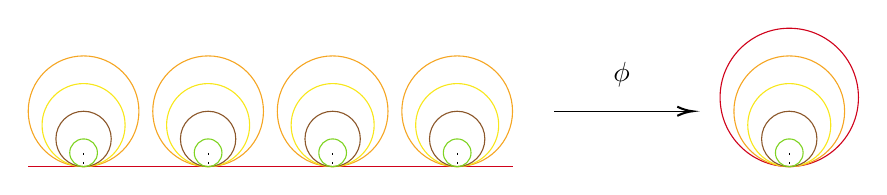
\begin{tikzpicture}[x=0.5pt,y=0.5pt,yscale=-1,xscale=1]
%uncomment if require: \path (0,300); %set diagram left start at 0, and has height of 300

%Shape: Circle [id:dp06397224202858343] 
\draw  [color={rgb, 255:red, 208; green, 2; blue, 27 }  ,draw opacity=1 ] (530,140) .. controls (530,112.39) and (552.39,90) .. (580,90) .. controls (607.61,90) and (630,112.39) .. (630,140) .. controls (630,167.61) and (607.61,190) .. (580,190) .. controls (552.39,190) and (530,167.61) .. (530,140) -- cycle ;
%Shape: Circle [id:dp2597096415804374] 
\draw  [color={rgb, 255:red, 245; green, 166; blue, 35 }  ,draw opacity=1 ] (540,150) .. controls (540,127.91) and (557.91,110) .. (580,110) .. controls (602.09,110) and (620,127.91) .. (620,150) .. controls (620,172.09) and (602.09,190) .. (580,190) .. controls (557.91,190) and (540,172.09) .. (540,150) -- cycle ;
%Shape: Circle [id:dp050005102637662446] 
\draw  [color={rgb, 255:red, 248; green, 231; blue, 28 }  ,draw opacity=1 ] (550,160) .. controls (550,143.43) and (563.43,130) .. (580,130) .. controls (596.57,130) and (610,143.43) .. (610,160) .. controls (610,176.57) and (596.57,190) .. (580,190) .. controls (563.43,190) and (550,176.57) .. (550,160) -- cycle ;
%Shape: Circle [id:dp5396637816931802] 
\draw  [color={rgb, 255:red, 139; green, 87; blue, 42 }  ,draw opacity=1 ] (560,170) .. controls (560,158.95) and (568.95,150) .. (580,150) .. controls (591.05,150) and (600,158.95) .. (600,170) .. controls (600,181.05) and (591.05,190) .. (580,190) .. controls (568.95,190) and (560,181.05) .. (560,170) -- cycle ;
%Shape: Circle [id:dp16156428674020806] 
\draw  [color={rgb, 255:red, 126; green, 211; blue, 33 }  ,draw opacity=1 ] (570,180) .. controls (570,174.48) and (574.48,170) .. (580,170) .. controls (585.52,170) and (590,174.48) .. (590,180) .. controls (590,185.52) and (585.52,190) .. (580,190) .. controls (574.48,190) and (570,185.52) .. (570,180) -- cycle ;
%Straight Lines [id:da03476842775885991] 
\draw  [dash pattern={on 0.84pt off 2.51pt}]  (580,180) -- (580,190) ;
%Straight Lines [id:da1462307798401159] 
\draw [color={rgb, 255:red, 208; green, 2; blue, 27 }  ,draw opacity=1 ]   (30,190) -- (380,190) ;
%Shape: Circle [id:dp2790215973041046] 
\draw  [color={rgb, 255:red, 245; green, 166; blue, 35 }  ,draw opacity=1 ] (30,150) .. controls (30,127.91) and (47.91,110) .. (70,110) .. controls (92.09,110) and (110,127.91) .. (110,150) .. controls (110,172.09) and (92.09,190) .. (70,190) .. controls (47.91,190) and (30,172.09) .. (30,150) -- cycle ;
%Shape: Circle [id:dp46259725537421914] 
\draw  [color={rgb, 255:red, 248; green, 231; blue, 28 }  ,draw opacity=1 ] (40,160) .. controls (40,143.43) and (53.43,130) .. (70,130) .. controls (86.57,130) and (100,143.43) .. (100,160) .. controls (100,176.57) and (86.57,190) .. (70,190) .. controls (53.43,190) and (40,176.57) .. (40,160) -- cycle ;
%Shape: Circle [id:dp5028036111113044] 
\draw  [color={rgb, 255:red, 139; green, 87; blue, 42 }  ,draw opacity=1 ] (50,170) .. controls (50,158.95) and (58.95,150) .. (70,150) .. controls (81.05,150) and (90,158.95) .. (90,170) .. controls (90,181.05) and (81.05,190) .. (70,190) .. controls (58.95,190) and (50,181.05) .. (50,170) -- cycle ;
%Shape: Circle [id:dp007872617843824314] 
\draw  [color={rgb, 255:red, 126; green, 211; blue, 33 }  ,draw opacity=1 ] (60,180) .. controls (60,174.48) and (64.48,170) .. (70,170) .. controls (75.52,170) and (80,174.48) .. (80,180) .. controls (80,185.52) and (75.52,190) .. (70,190) .. controls (64.48,190) and (60,185.52) .. (60,180) -- cycle ;
%Straight Lines [id:da1373403977007781] 
\draw  [dash pattern={on 0.84pt off 2.51pt}]  (70,180) -- (70,190) ;

%Shape: Circle [id:dp006597295703618999] 
\draw  [color={rgb, 255:red, 245; green, 166; blue, 35 }  ,draw opacity=1 ] (120,150) .. controls (120,127.91) and (137.91,110) .. (160,110) .. controls (182.09,110) and (200,127.91) .. (200,150) .. controls (200,172.09) and (182.09,190) .. (160,190) .. controls (137.91,190) and (120,172.09) .. (120,150) -- cycle ;
%Shape: Circle [id:dp08990508225264682] 
\draw  [color={rgb, 255:red, 248; green, 231; blue, 28 }  ,draw opacity=1 ] (130,160) .. controls (130,143.43) and (143.43,130) .. (160,130) .. controls (176.57,130) and (190,143.43) .. (190,160) .. controls (190,176.57) and (176.57,190) .. (160,190) .. controls (143.43,190) and (130,176.57) .. (130,160) -- cycle ;
%Shape: Circle [id:dp20764231446031645] 
\draw  [color={rgb, 255:red, 139; green, 87; blue, 42 }  ,draw opacity=1 ] (140,170) .. controls (140,158.95) and (148.95,150) .. (160,150) .. controls (171.05,150) and (180,158.95) .. (180,170) .. controls (180,181.05) and (171.05,190) .. (160,190) .. controls (148.95,190) and (140,181.05) .. (140,170) -- cycle ;
%Shape: Circle [id:dp5988240568896183] 
\draw  [color={rgb, 255:red, 126; green, 211; blue, 33 }  ,draw opacity=1 ] (150,180) .. controls (150,174.48) and (154.48,170) .. (160,170) .. controls (165.52,170) and (170,174.48) .. (170,180) .. controls (170,185.52) and (165.52,190) .. (160,190) .. controls (154.48,190) and (150,185.52) .. (150,180) -- cycle ;
%Straight Lines [id:da3606442931428455] 
\draw  [dash pattern={on 0.84pt off 2.51pt}]  (160,180) -- (160,190) ;

%Shape: Circle [id:dp11202226460574205] 
\draw  [color={rgb, 255:red, 245; green, 166; blue, 35 }  ,draw opacity=1 ] (210,150) .. controls (210,127.91) and (227.91,110) .. (250,110) .. controls (272.09,110) and (290,127.91) .. (290,150) .. controls (290,172.09) and (272.09,190) .. (250,190) .. controls (227.91,190) and (210,172.09) .. (210,150) -- cycle ;
%Shape: Circle [id:dp11640395230770162] 
\draw  [color={rgb, 255:red, 248; green, 231; blue, 28 }  ,draw opacity=1 ] (220,160) .. controls (220,143.43) and (233.43,130) .. (250,130) .. controls (266.57,130) and (280,143.43) .. (280,160) .. controls (280,176.57) and (266.57,190) .. (250,190) .. controls (233.43,190) and (220,176.57) .. (220,160) -- cycle ;
%Shape: Circle [id:dp876229513121312] 
\draw  [color={rgb, 255:red, 139; green, 87; blue, 42 }  ,draw opacity=1 ] (230,170) .. controls (230,158.95) and (238.95,150) .. (250,150) .. controls (261.05,150) and (270,158.95) .. (270,170) .. controls (270,181.05) and (261.05,190) .. (250,190) .. controls (238.95,190) and (230,181.05) .. (230,170) -- cycle ;
%Shape: Circle [id:dp39170681409117203] 
\draw  [color={rgb, 255:red, 126; green, 211; blue, 33 }  ,draw opacity=1 ] (240,180) .. controls (240,174.48) and (244.48,170) .. (250,170) .. controls (255.52,170) and (260,174.48) .. (260,180) .. controls (260,185.52) and (255.52,190) .. (250,190) .. controls (244.48,190) and (240,185.52) .. (240,180) -- cycle ;
%Straight Lines [id:da5965835992522015] 
\draw  [dash pattern={on 0.84pt off 2.51pt}]  (250,180) -- (250,190) ;

%Shape: Circle [id:dp40419390391548393] 
\draw  [color={rgb, 255:red, 245; green, 166; blue, 35 }  ,draw opacity=1 ] (300,150) .. controls (300,127.91) and (317.91,110) .. (340,110) .. controls (362.09,110) and (380,127.91) .. (380,150) .. controls (380,172.09) and (362.09,190) .. (340,190) .. controls (317.91,190) and (300,172.09) .. (300,150) -- cycle ;
%Shape: Circle [id:dp17267660646482663] 
\draw  [color={rgb, 255:red, 248; green, 231; blue, 28 }  ,draw opacity=1 ] (310,160) .. controls (310,143.43) and (323.43,130) .. (340,130) .. controls (356.57,130) and (370,143.43) .. (370,160) .. controls (370,176.57) and (356.57,190) .. (340,190) .. controls (323.43,190) and (310,176.57) .. (310,160) -- cycle ;
%Shape: Circle [id:dp9801906341081632] 
\draw  [color={rgb, 255:red, 139; green, 87; blue, 42 }  ,draw opacity=1 ] (320,170) .. controls (320,158.95) and (328.95,150) .. (340,150) .. controls (351.05,150) and (360,158.95) .. (360,170) .. controls (360,181.05) and (351.05,190) .. (340,190) .. controls (328.95,190) and (320,181.05) .. (320,170) -- cycle ;
%Shape: Circle [id:dp42389912940336316] 
\draw  [color={rgb, 255:red, 126; green, 211; blue, 33 }  ,draw opacity=1 ] (330,180) .. controls (330,174.48) and (334.48,170) .. (340,170) .. controls (345.52,170) and (350,174.48) .. (350,180) .. controls (350,185.52) and (345.52,190) .. (340,190) .. controls (334.48,190) and (330,185.52) .. (330,180) -- cycle ;
%Straight Lines [id:da4314324982083172] 
\draw  [dash pattern={on 0.84pt off 2.51pt}]  (340,180) -- (340,190) ;

%Straight Lines [id:da8526374743770496] 
\draw    (410,150) -- (508,150) ;
\draw [shift={(510,150)}, rotate = 180] [color={rgb, 255:red, 0; green, 0; blue, 0 }  ][line width=0.75]    (10.93,-3.29) .. controls (6.95,-1.4) and (3.31,-0.3) .. (0,0) .. controls (3.31,0.3) and (6.95,1.4) .. (10.93,3.29)   ;

% Text Node
\draw (451,112.4) node [anchor=north west][inner sep=0.75pt]    {$\phi $};


\end{tikzpicture}

  

\end{center}
\end{frame}


\begin{frame}{Construction of $Z$}
Set \textcolor{colororange}{$S_n=\{z:|z-1/2n|=1/2n,arg(z-1/2)\in[-\pi/2,\pi/2]\}$}
We define \textcolor{colororange}{$Z$} as follows:
\begin{footnotesize}
    \textcolor{colororange}{
    \begin{align*}
      Z=\bigcup_{z\in\mathbb{Z}}&\left(\left[z-\frac{1}{2},z+\frac{1}{2}\right]\times{0}\cup\left[z-\frac{1}{2},z+\frac{1}{2}\right]\times{2}\right.\\
      &\cup\left(\bigcup_{n>|Z|}(C_n+z)\right)\cup\left(\bigcup_{n>|Z|}(2-C_n+z)\right)\\
      &\cup\left(\bigcup_{n=1}^{|z|}(S_n+z)\right)\cup\left(\bigcup_{n=1}^{|z|}(2-S_n+z)\right)\\
      &\cup\left(\bigcup_{n=1}^{|z|}\{z-1/n\}\times [1/n,2-1/n]\right)\\
      &\left.\cup\left(\bigcup_{n=1}^{|z|}\{z+1/n\}\times [1/n,2-1/n]\right)\right)\\
    \end{align*}}
\end{footnotesize}
\end{frame}

\begin{frame}{Construction of $Z$}
    Which looks like the following:
\begin{center}


\tikzset{every picture/.style={line width=0.75pt}} %set default line width to 0.75pt        

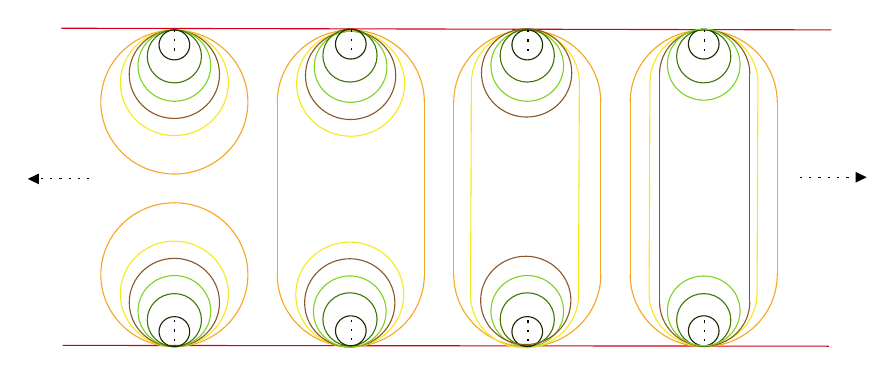
\begin{tikzpicture}[x=0.45pt,y=0.45pt,yscale=-1,xscale=1]
%uncomment if require: \path (0,330); %set diagram left start at 0, and has height of 330

%Straight Lines [id:da8019268829751769] 
\draw [color={rgb, 255:red, 208; green, 2; blue, 27 }  ,draw opacity=1 ]   (40,297.67) -- (655.33,298.33) ;
%Straight Lines [id:da19411018003149527] 
\draw [color={rgb, 255:red, 208; green, 2; blue, 27 }  ,draw opacity=1 ]   (39,43) -- (657.33,44.33) ;
%Shape: Ellipse [id:dp755042607694153] 
\draw  [color={rgb, 255:red, 245; green, 166; blue, 35 }  ,draw opacity=1 ] (70.67,240.92) .. controls (70.67,209.02) and (97.1,183.17) .. (129.7,183.17) .. controls (162.31,183.17) and (188.74,209.02) .. (188.74,240.92) .. controls (188.74,272.82) and (162.31,298.68) .. (129.7,298.68) .. controls (97.1,298.68) and (70.67,272.82) .. (70.67,240.92) -- cycle ;
%Shape: Ellipse [id:dp8592507789171753] 
\draw  [color={rgb, 255:red, 245; green, 166; blue, 35 }  ,draw opacity=1 ] (70.67,102.31) .. controls (70.67,70.41) and (97.1,44.55) .. (129.7,44.55) .. controls (162.31,44.55) and (188.74,70.41) .. (188.74,102.31) .. controls (188.74,134.21) and (162.31,160.06) .. (129.7,160.06) .. controls (97.1,160.06) and (70.67,134.21) .. (70.67,102.31) -- cycle ;
%Shape: Arc [id:dp5575659847483159] 
\draw  [draw opacity=0] (212.35,102.31) .. controls (212.35,70.41) and (238.79,44.55) .. (271.39,44.55) .. controls (304,44.55) and (330.43,70.41) .. (330.43,102.31) -- (271.39,102.31) -- cycle ; \draw  [color={rgb, 255:red, 245; green, 166; blue, 35 }  ,draw opacity=1 ] (212.35,102.31) .. controls (212.35,70.41) and (238.79,44.55) .. (271.39,44.55) .. controls (304,44.55) and (330.43,70.41) .. (330.43,102.31) ;  
%Shape: Arc [id:dp7393184648450104] 
\draw  [draw opacity=0] (330.43,240.92) .. controls (330.43,272.82) and (304,298.68) .. (271.39,298.68) .. controls (238.79,298.68) and (212.35,272.82) .. (212.35,240.92) -- (271.39,240.92) -- cycle ; \draw  [color={rgb, 255:red, 245; green, 166; blue, 35 }  ,draw opacity=1 ] (330.43,240.92) .. controls (330.43,272.82) and (304,298.68) .. (271.39,298.68) .. controls (238.79,298.68) and (212.35,272.82) .. (212.35,240.92) ;  
%Straight Lines [id:da6912455869646965] 
\draw [color={rgb, 255:red, 245; green, 166; blue, 35 }  ,draw opacity=1 ]   (212.35,102.31) -- (212.35,240.92) ;
%Straight Lines [id:da7415674220693267] 
\draw [color={rgb, 255:red, 245; green, 166; blue, 35 }  ,draw opacity=1 ]   (330.43,102.31) -- (330.43,240.92) ;
%Shape: Arc [id:dp2844251535638781] 
\draw  [draw opacity=0] (354.04,102.31) .. controls (354.04,70.41) and (380.47,44.55) .. (413.08,44.55) .. controls (445.68,44.55) and (472.12,70.41) .. (472.12,102.31) -- (413.08,102.31) -- cycle ; \draw  [color={rgb, 255:red, 245; green, 166; blue, 35 }  ,draw opacity=1 ] (354.04,102.31) .. controls (354.04,70.41) and (380.47,44.55) .. (413.08,44.55) .. controls (445.68,44.55) and (472.12,70.41) .. (472.12,102.31) ;  
%Shape: Arc [id:dp07026080518879607] 
\draw  [draw opacity=0] (472.12,240.92) .. controls (472.12,272.82) and (445.68,298.68) .. (413.08,298.68) .. controls (380.47,298.68) and (354.04,272.82) .. (354.04,240.92) -- (413.08,240.92) -- cycle ; \draw  [color={rgb, 255:red, 245; green, 166; blue, 35 }  ,draw opacity=1 ] (472.12,240.92) .. controls (472.12,272.82) and (445.68,298.68) .. (413.08,298.68) .. controls (380.47,298.68) and (354.04,272.82) .. (354.04,240.92) ;  
%Straight Lines [id:da4228728984431098] 
\draw [color={rgb, 255:red, 245; green, 166; blue, 35 }  ,draw opacity=1 ]   (354.04,102.31) -- (354.04,240.92) ;
%Straight Lines [id:da010401618689007575] 
\draw [color={rgb, 255:red, 245; green, 166; blue, 35 }  ,draw opacity=1 ]   (472.12,102.31) -- (472.12,240.92) ;
%Shape: Arc [id:dp5665130655467749] 
\draw  [draw opacity=0] (495.73,102.31) .. controls (495.73,70.41) and (522.16,44.55) .. (554.77,44.55) .. controls (587.37,44.55) and (613.8,70.41) .. (613.8,102.31) -- (554.77,102.31) -- cycle ; \draw  [color={rgb, 255:red, 245; green, 166; blue, 35 }  ,draw opacity=1 ] (495.73,102.31) .. controls (495.73,70.41) and (522.16,44.55) .. (554.77,44.55) .. controls (587.37,44.55) and (613.8,70.41) .. (613.8,102.31) ;  
%Shape: Arc [id:dp45839677289396485] 
\draw  [draw opacity=0] (613.8,240.92) .. controls (613.8,272.82) and (587.37,298.68) .. (554.77,298.68) .. controls (522.16,298.68) and (495.73,272.82) .. (495.73,240.92) -- (554.77,240.92) -- cycle ; \draw  [color={rgb, 255:red, 245; green, 166; blue, 35 }  ,draw opacity=1 ] (613.8,240.92) .. controls (613.8,272.82) and (587.37,298.68) .. (554.77,298.68) .. controls (522.16,298.68) and (495.73,272.82) .. (495.73,240.92) ;  
%Straight Lines [id:da9775394006068312] 
\draw [color={rgb, 255:red, 245; green, 166; blue, 35 }  ,draw opacity=1 ]   (495.73,102.31) -- (495.73,240.92) ;
%Straight Lines [id:da8522804711696934] 
\draw [color={rgb, 255:red, 245; green, 166; blue, 35 }  ,draw opacity=1 ]   (613.8,102.31) -- (613.8,240.92) ;
%Shape: Ellipse [id:dp7061775084823935] 
\draw  [color={rgb, 255:red, 248; green, 231; blue, 28 }  ,draw opacity=1 ] (227.87,87.57) .. controls (227.87,64.29) and (247.28,45.42) .. (271.22,45.42) .. controls (295.16,45.42) and (314.57,64.29) .. (314.57,87.57) .. controls (314.57,110.86) and (295.16,129.73) .. (271.22,129.73) .. controls (247.28,129.73) and (227.87,110.86) .. (227.87,87.57) -- cycle ;
%Shape: Ellipse [id:dp18615492139699985] 
\draw  [color={rgb, 255:red, 248; green, 231; blue, 28 }  ,draw opacity=1 ] (227.2,256.85) .. controls (227.2,233.57) and (246.61,214.7) .. (270.55,214.7) .. controls (294.49,214.7) and (313.9,233.57) .. (313.9,256.85) .. controls (313.9,280.13) and (294.49,299.01) .. (270.55,299.01) .. controls (246.61,299.01) and (227.2,280.13) .. (227.2,256.85) -- cycle ;
%Shape: Arc [id:dp8538635445684597] 
\draw  [draw opacity=0] (368.21,86.96) .. controls (368.21,86.96) and (368.21,86.96) .. (368.21,86.96) .. controls (368.21,63.54) and (387.62,44.55) .. (411.56,44.55) .. controls (435.5,44.55) and (454.91,63.54) .. (454.91,86.96) -- (411.56,86.96) -- cycle ; \draw  [color={rgb, 255:red, 248; green, 231; blue, 28 }  ,draw opacity=1 ] (368.21,86.96) .. controls (368.21,86.96) and (368.21,86.96) .. (368.21,86.96) .. controls (368.21,63.54) and (387.62,44.55) .. (411.56,44.55) .. controls (435.5,44.55) and (454.91,63.54) .. (454.91,86.96) ;  
%Shape: Arc [id:dp49810715044832066] 
\draw  [draw opacity=0] (454.24,257.26) .. controls (454.24,257.26) and (454.24,257.26) .. (454.24,257.26) .. controls (454.24,280.68) and (434.83,299.67) .. (410.89,299.67) .. controls (386.95,299.67) and (367.54,280.68) .. (367.54,257.26) -- (410.89,257.26) -- cycle ; \draw  [color={rgb, 255:red, 248; green, 231; blue, 28 }  ,draw opacity=1 ] (454.24,257.26) .. controls (454.24,257.26) and (454.24,257.26) .. (454.24,257.26) .. controls (454.24,280.68) and (434.83,299.67) .. (410.89,299.67) .. controls (386.95,299.67) and (367.54,280.68) .. (367.54,257.26) ;  
%Straight Lines [id:da06818006829326317] 
\draw [color={rgb, 255:red, 248; green, 231; blue, 28 }  ,draw opacity=1 ]   (368.21,86.96) -- (367.54,257.26) ;
%Straight Lines [id:da9641952746953396] 
\draw [color={rgb, 255:red, 248; green, 231; blue, 28 }  ,draw opacity=1 ]   (454.91,86.96) -- (454.24,257.26) ;

%Shape: Arc [id:dp5750096331920825] 
\draw  [draw opacity=0] (511.59,86.69) .. controls (511.59,63.42) and (530.99,44.55) .. (554.94,44.55) .. controls (578.88,44.55) and (598.29,63.42) .. (598.29,86.69) -- (554.94,86.69) -- cycle ; \draw  [color={rgb, 255:red, 248; green, 231; blue, 28 }  ,draw opacity=1 ] (511.59,86.69) .. controls (511.59,63.42) and (530.99,44.55) .. (554.94,44.55) .. controls (578.88,44.55) and (598.29,63.42) .. (598.29,86.69) ;  
%Shape: Arc [id:dp4452867146415097] 
\draw  [draw opacity=0] (597.61,255.88) .. controls (597.61,279.15) and (578.2,298.02) .. (554.26,298.02) .. controls (530.32,298.02) and (510.91,279.15) .. (510.91,255.88) -- (554.26,255.88) -- cycle ; \draw  [color={rgb, 255:red, 248; green, 231; blue, 28 }  ,draw opacity=1 ] (597.61,255.88) .. controls (597.61,279.15) and (578.2,298.02) .. (554.26,298.02) .. controls (530.32,298.02) and (510.91,279.15) .. (510.91,255.88) ;  
%Straight Lines [id:da47654812565410376] 
\draw [color={rgb, 255:red, 248; green, 231; blue, 28 }  ,draw opacity=1 ]   (511.59,86.69) -- (510.91,255.88) ;
%Straight Lines [id:da3541247537262896] 
\draw [color={rgb, 255:red, 248; green, 231; blue, 28 }  ,draw opacity=1 ]   (598.29,86.69) -- (597.61,255.88) ;

%Shape: Ellipse [id:dp015112826866313211] 
\draw  [color={rgb, 255:red, 248; green, 231; blue, 28 }  ,draw opacity=1 ] (86.35,86.9) .. controls (86.35,63.51) and (105.76,44.55) .. (129.7,44.55) .. controls (153.64,44.55) and (173.05,63.51) .. (173.05,86.9) .. controls (173.05,110.29) and (153.64,129.25) .. (129.7,129.25) .. controls (105.76,129.25) and (86.35,110.29) .. (86.35,86.9) -- cycle ;
%Shape: Ellipse [id:dp08480110306864375] 
\draw  [color={rgb, 255:red, 248; green, 231; blue, 28 }  ,draw opacity=1 ] (86.35,256.33) .. controls (86.35,232.94) and (105.76,213.98) .. (129.7,213.98) .. controls (153.64,213.98) and (173.05,232.94) .. (173.05,256.33) .. controls (173.05,279.72) and (153.64,298.68) .. (129.7,298.68) .. controls (105.76,298.68) and (86.35,279.72) .. (86.35,256.33) -- cycle ;
%Shape: Ellipse [id:dp6396517846512791] 
\draw  [color={rgb, 255:red, 139; green, 87; blue, 42 }  ,draw opacity=1 ] (93.47,80) .. controls (93.47,60.42) and (109.69,44.55) .. (129.7,44.55) .. controls (149.71,44.55) and (165.94,60.42) .. (165.94,80) .. controls (165.94,99.58) and (149.71,115.45) .. (129.7,115.45) .. controls (109.69,115.45) and (93.47,99.58) .. (93.47,80) -- cycle ;
%Shape: Ellipse [id:dp26863757459073234] 
\draw  [color={rgb, 255:red, 139; green, 87; blue, 42 }  ,draw opacity=1 ] (93.47,263.23) .. controls (93.47,243.65) and (109.69,227.78) .. (129.7,227.78) .. controls (149.71,227.78) and (165.94,243.65) .. (165.94,263.23) .. controls (165.94,282.81) and (149.71,298.68) .. (129.7,298.68) .. controls (109.69,298.68) and (93.47,282.81) .. (93.47,263.23) -- cycle ;
%Shape: Ellipse [id:dp6888221898815015] 
\draw  [color={rgb, 255:red, 139; green, 87; blue, 42 }  ,draw opacity=1 ] (234.99,80.87) .. controls (234.99,61.29) and (251.21,45.42) .. (271.22,45.42) .. controls (291.23,45.42) and (307.46,61.29) .. (307.46,80.87) .. controls (307.46,100.44) and (291.23,116.31) .. (271.22,116.31) .. controls (251.21,116.31) and (234.99,100.44) .. (234.99,80.87) -- cycle ;
%Shape: Ellipse [id:dp6131335458949229] 
\draw  [color={rgb, 255:red, 139; green, 87; blue, 42 }  ,draw opacity=1 ] (234.31,263.56) .. controls (234.31,243.98) and (250.54,228.11) .. (270.55,228.11) .. controls (290.56,228.11) and (306.78,243.98) .. (306.78,263.56) .. controls (306.78,283.14) and (290.56,299.01) .. (270.55,299.01) .. controls (250.54,299.01) and (234.31,283.14) .. (234.31,263.56) -- cycle ;
%Shape: Arc [id:dp06200106763647828] 
\draw  [draw opacity=0] (519.32,79.62) .. controls (519.32,79.62) and (519.32,79.62) .. (519.32,79.62) .. controls (519.32,60.04) and (535.54,44.17) .. (555.55,44.17) .. controls (575.57,44.17) and (591.79,60.04) .. (591.79,79.62) -- (555.55,79.62) -- cycle ; \draw  [color={rgb, 255:red, 139; green, 87; blue, 42 }  ,draw opacity=1 ] (519.32,79.62) .. controls (519.32,79.62) and (519.32,79.62) .. (519.32,79.62) .. controls (519.32,60.04) and (535.54,44.17) .. (555.55,44.17) .. controls (575.57,44.17) and (591.79,60.04) .. (591.79,79.62) ;  
%Shape: Arc [id:dp5244952406542043] 
\draw  [draw opacity=0] (591.79,262.84) .. controls (591.79,262.84) and (591.79,262.84) .. (591.79,262.84) .. controls (591.79,282.42) and (575.57,298.29) .. (555.55,298.29) .. controls (535.54,298.29) and (519.32,282.42) .. (519.32,262.84) -- (555.55,262.84) -- cycle ; \draw  [color={rgb, 255:red, 139; green, 87; blue, 42 }  ,draw opacity=1 ] (591.79,262.84) .. controls (591.79,262.84) and (591.79,262.84) .. (591.79,262.84) .. controls (591.79,282.42) and (575.57,298.29) .. (555.55,298.29) .. controls (535.54,298.29) and (519.32,282.42) .. (519.32,262.84) ;  
%Straight Lines [id:da7525466584384344] 
\draw [color={rgb, 255:red, 139; green, 87; blue, 42 }  ,draw opacity=1 ]   (519.32,79.62) -- (519.32,262.84) ;
%Straight Lines [id:da25122929214675105] 
\draw [color={rgb, 255:red, 139; green, 87; blue, 42 }  ,draw opacity=1 ]   (591.79,80) -- (591.79,263.23) ;

%Shape: Ellipse [id:dp9916809302488827] 
\draw  [color={rgb, 255:red, 126; green, 211; blue, 33 }  ,draw opacity=1 ] (100.52,73.1) .. controls (100.52,57.33) and (113.59,44.55) .. (129.7,44.55) .. controls (145.82,44.55) and (158.88,57.33) .. (158.88,73.1) .. controls (158.88,88.87) and (145.82,101.65) .. (129.7,101.65) .. controls (113.59,101.65) and (100.52,88.87) .. (100.52,73.1) -- cycle ;
%Shape: Ellipse [id:dp21228108456554207] 
\draw  [color={rgb, 255:red, 126; green, 211; blue, 33 }  ,draw opacity=1 ] (100.52,270.13) .. controls (100.52,254.36) and (113.59,241.58) .. (129.7,241.58) .. controls (145.82,241.58) and (158.88,254.36) .. (158.88,270.13) .. controls (158.88,285.9) and (145.82,298.68) .. (129.7,298.68) .. controls (113.59,298.68) and (100.52,285.9) .. (100.52,270.13) -- cycle ;
%Shape: Ellipse [id:dp08651193901107368] 
\draw  [color={rgb, 255:red, 126; green, 211; blue, 33 }  ,draw opacity=1 ] (242.04,73.97) .. controls (242.04,58.2) and (255.11,45.42) .. (271.22,45.42) .. controls (287.34,45.42) and (300.4,58.2) .. (300.4,73.97) .. controls (300.4,89.73) and (287.34,102.51) .. (271.22,102.51) .. controls (255.11,102.51) and (242.04,89.73) .. (242.04,73.97) -- cycle ;
%Shape: Ellipse [id:dp6967140272448221] 
\draw  [color={rgb, 255:red, 126; green, 211; blue, 33 }  ,draw opacity=1 ] (241.37,270.46) .. controls (241.37,254.69) and (254.43,241.91) .. (270.55,241.91) .. controls (286.66,241.91) and (299.73,254.69) .. (299.73,270.46) .. controls (299.73,286.23) and (286.66,299.01) .. (270.55,299.01) .. controls (254.43,299.01) and (241.37,286.23) .. (241.37,270.46) -- cycle ;
%Shape: Ellipse [id:dp3442874649468213] 
\draw  [color={rgb, 255:red, 126; green, 211; blue, 33 }  ,draw opacity=1 ] (383.9,73.1) .. controls (383.9,57.33) and (396.96,44.55) .. (413.08,44.55) .. controls (429.2,44.55) and (442.26,57.33) .. (442.26,73.1) .. controls (442.26,88.87) and (429.2,101.65) .. (413.08,101.65) .. controls (396.96,101.65) and (383.9,88.87) .. (383.9,73.1) -- cycle ;
%Shape: Ellipse [id:dp04347435390523402] 
\draw  [color={rgb, 255:red, 126; green, 211; blue, 33 }  ,draw opacity=1 ] (383.9,270.13) .. controls (383.9,254.36) and (396.96,241.58) .. (413.08,241.58) .. controls (429.2,241.58) and (442.26,254.36) .. (442.26,270.13) .. controls (442.26,285.9) and (429.2,298.68) .. (413.08,298.68) .. controls (396.96,298.68) and (383.9,285.9) .. (383.9,270.13) -- cycle ;
%Shape: Ellipse [id:dp26123086484050506] 
\draw  [color={rgb, 255:red, 65; green, 117; blue, 5 }  ,draw opacity=1 ] (107.94,65.61) .. controls (107.94,53.86) and (117.69,44.33) .. (129.7,44.33) .. controls (141.72,44.33) and (151.46,53.86) .. (151.46,65.61) .. controls (151.46,77.37) and (141.72,86.9) .. (129.7,86.9) .. controls (117.69,86.9) and (107.94,77.37) .. (107.94,65.61) -- cycle ;
%Shape: Ellipse [id:dp09091362212598297] 
\draw  [color={rgb, 255:red, 65; green, 117; blue, 5 }  ,draw opacity=1 ] (107.94,277.39) .. controls (107.94,265.63) and (117.69,256.1) .. (129.7,256.1) .. controls (141.72,256.1) and (151.46,265.63) .. (151.46,277.39) .. controls (151.46,289.15) and (141.72,298.68) .. (129.7,298.68) .. controls (117.69,298.68) and (107.94,289.15) .. (107.94,277.39) -- cycle ;
%Shape: Ellipse [id:dp3767844311743297] 
\draw  [color={rgb, 255:red, 65; green, 117; blue, 5 }  ,draw opacity=1 ] (248.96,64.95) .. controls (248.96,53.2) and (258.7,43.67) .. (270.72,43.67) .. controls (282.73,43.67) and (292.48,53.2) .. (292.48,64.95) .. controls (292.48,76.71) and (282.73,86.24) .. (270.72,86.24) .. controls (258.7,86.24) and (248.96,76.71) .. (248.96,64.95) -- cycle ;
%Shape: Ellipse [id:dp03544985956989655] 
\draw  [color={rgb, 255:red, 65; green, 117; blue, 5 }  ,draw opacity=1 ] (248.96,276.73) .. controls (248.96,264.97) and (258.7,255.44) .. (270.72,255.44) .. controls (282.73,255.44) and (292.48,264.97) .. (292.48,276.73) .. controls (292.48,288.49) and (282.73,298.02) .. (270.72,298.02) .. controls (258.7,298.02) and (248.96,288.49) .. (248.96,276.73) -- cycle ;
%Shape: Ellipse [id:dp06917760052791733] 
\draw  [color={rgb, 255:red, 65; green, 117; blue, 5 }  ,draw opacity=1 ] (391.32,64.95) .. controls (391.32,53.2) and (401.06,43.67) .. (413.08,43.67) .. controls (425.1,43.67) and (434.84,53.2) .. (434.84,64.95) .. controls (434.84,76.71) and (425.1,86.24) .. (413.08,86.24) .. controls (401.06,86.24) and (391.32,76.71) .. (391.32,64.95) -- cycle ;
%Shape: Ellipse [id:dp9282575291068949] 
\draw  [color={rgb, 255:red, 65; green, 117; blue, 5 }  ,draw opacity=1 ] (391.32,276.73) .. controls (391.32,264.97) and (401.06,255.44) .. (413.08,255.44) .. controls (425.1,255.44) and (434.84,264.97) .. (434.84,276.73) .. controls (434.84,288.49) and (425.1,298.02) .. (413.08,298.02) .. controls (401.06,298.02) and (391.32,288.49) .. (391.32,276.73) -- cycle ;
%Shape: Ellipse [id:dp07195796370829588] 
\draw  [color={rgb, 255:red, 65; green, 117; blue, 5 }  ,draw opacity=1 ] (533.01,65.61) .. controls (533.01,53.86) and (542.75,44.33) .. (554.77,44.33) .. controls (566.78,44.33) and (576.53,53.86) .. (576.53,65.61) .. controls (576.53,77.37) and (566.78,86.9) .. (554.77,86.9) .. controls (542.75,86.9) and (533.01,77.37) .. (533.01,65.61) -- cycle ;
%Shape: Ellipse [id:dp5724266197209639] 
\draw  [color={rgb, 255:red, 65; green, 117; blue, 5 }  ,draw opacity=1 ] (533.01,277.39) .. controls (533.01,265.63) and (542.75,256.1) .. (554.77,256.1) .. controls (566.78,256.1) and (576.53,265.63) .. (576.53,277.39) .. controls (576.53,289.15) and (566.78,298.68) .. (554.77,298.68) .. controls (542.75,298.68) and (533.01,289.15) .. (533.01,277.39) -- cycle ;
%Shape: Ellipse [id:dp5350672711499449] 
\draw  [color={rgb, 255:red, 22; green, 42; blue, 1 }  ,draw opacity=1 ] (117.39,56.37) .. controls (117.39,49.72) and (122.9,44.33) .. (129.7,44.33) .. controls (136.5,44.33) and (142.02,49.72) .. (142.02,56.37) .. controls (142.02,63.03) and (136.5,68.42) .. (129.7,68.42) .. controls (122.9,68.42) and (117.39,63.03) .. (117.39,56.37) -- cycle ;
%Shape: Ellipse [id:dp44217018518301565] 
\draw  [color={rgb, 255:red, 22; green, 42; blue, 1 }  ,draw opacity=1 ] (117.39,286.63) .. controls (117.39,279.98) and (122.9,274.58) .. (129.7,274.58) .. controls (136.5,274.58) and (142.02,279.98) .. (142.02,286.63) .. controls (142.02,293.28) and (136.5,298.68) .. (129.7,298.68) .. controls (122.9,298.68) and (117.39,293.28) .. (117.39,286.63) -- cycle ;
%Shape: Ellipse [id:dp2098277175532065] 
\draw  [color={rgb, 255:red, 22; green, 42; blue, 1 }  ,draw opacity=1 ] (259.08,55.71) .. controls (259.08,49.06) and (264.59,43.67) .. (271.39,43.67) .. controls (278.19,43.67) and (283.7,49.06) .. (283.7,55.71) .. controls (283.7,62.37) and (278.19,67.76) .. (271.39,67.76) .. controls (264.59,67.76) and (259.08,62.37) .. (259.08,55.71) -- cycle ;
%Shape: Ellipse [id:dp8563776640680607] 
\draw  [color={rgb, 255:red, 22; green, 42; blue, 1 }  ,draw opacity=1 ] (259.08,285.97) .. controls (259.08,279.32) and (264.59,273.92) .. (271.39,273.92) .. controls (278.19,273.92) and (283.7,279.32) .. (283.7,285.97) .. controls (283.7,292.62) and (278.19,298.02) .. (271.39,298.02) .. controls (264.59,298.02) and (259.08,292.62) .. (259.08,285.97) -- cycle ;
%Shape: Ellipse [id:dp17239593316849888] 
\draw  [color={rgb, 255:red, 22; green, 42; blue, 1 }  ,draw opacity=1 ] (400.77,56.37) .. controls (400.77,49.72) and (406.28,44.33) .. (413.08,44.33) .. controls (419.88,44.33) and (425.39,49.72) .. (425.39,56.37) .. controls (425.39,63.03) and (419.88,68.42) .. (413.08,68.42) .. controls (406.28,68.42) and (400.77,63.03) .. (400.77,56.37) -- cycle ;
%Shape: Ellipse [id:dp9221214438967847] 
\draw  [color={rgb, 255:red, 22; green, 42; blue, 1 }  ,draw opacity=1 ] (400.77,286.63) .. controls (400.77,279.98) and (406.28,274.58) .. (413.08,274.58) .. controls (419.88,274.58) and (425.39,279.98) .. (425.39,286.63) .. controls (425.39,293.28) and (419.88,298.68) .. (413.08,298.68) .. controls (406.28,298.68) and (400.77,293.28) .. (400.77,286.63) -- cycle ;
%Shape: Ellipse [id:dp7717878656733393] 
\draw  [color={rgb, 255:red, 22; green, 42; blue, 1 }  ,draw opacity=1 ] (542.45,55.71) .. controls (542.45,49.06) and (547.97,43.67) .. (554.77,43.67) .. controls (561.57,43.67) and (567.08,49.06) .. (567.08,55.71) .. controls (567.08,62.37) and (561.57,67.76) .. (554.77,67.76) .. controls (547.97,67.76) and (542.45,62.37) .. (542.45,55.71) -- cycle ;
%Shape: Ellipse [id:dp023181803110648436] 
\draw  [color={rgb, 255:red, 22; green, 42; blue, 1 }  ,draw opacity=1 ] (542.45,285.97) .. controls (542.45,279.32) and (547.97,273.92) .. (554.77,273.92) .. controls (561.57,273.92) and (567.08,279.32) .. (567.08,285.97) .. controls (567.08,292.62) and (561.57,298.02) .. (554.77,298.02) .. controls (547.97,298.02) and (542.45,292.62) .. (542.45,285.97) -- cycle ;
%Straight Lines [id:da3971902588574284] 
\draw  [dash pattern={on 0.84pt off 2.51pt}]  (129.7,44.33) -- (129.7,65.61) ;
%Straight Lines [id:da42843264406748816] 
\draw  [dash pattern={on 0.84pt off 2.51pt}]  (129.7,277.39) -- (129.7,298.68) ;
%Straight Lines [id:da37965867604678805] 
\draw  [dash pattern={on 0.84pt off 2.51pt}]  (271.99,43.9) -- (271.99,65.18) ;
%Straight Lines [id:da46421804971724734] 
\draw  [dash pattern={on 0.84pt off 2.51pt}]  (271.99,276.96) -- (271.99,298.25) ;
%Straight Lines [id:da38984619285948274] 
\draw  [dash pattern={on 0.84pt off 2.51pt}]  (413.7,44.46) -- (413.7,65.75) ;
%Straight Lines [id:da16765663625080263] 
\draw  [dash pattern={on 0.84pt off 2.51pt}]  (413.7,277.53) -- (413.7,298.81) ;
%Straight Lines [id:da1739151256946022] 
\draw  [dash pattern={on 0.84pt off 2.51pt}]  (555.41,44.46) -- (555.41,65.75) ;
%Straight Lines [id:da30219095449842914] 
\draw  [dash pattern={on 0.84pt off 2.51pt}]  (555.41,277.53) -- (555.41,298.81) ;
%Shape: Ellipse [id:dp918610407888359] 
\draw  [color={rgb, 255:red, 139; green, 87; blue, 42 }  ,draw opacity=1 ] (376.32,78.86) .. controls (376.32,59.28) and (392.54,43.41) .. (412.56,43.41) .. controls (432.57,43.41) and (448.79,59.28) .. (448.79,78.86) .. controls (448.79,98.44) and (432.57,114.31) .. (412.56,114.31) .. controls (392.54,114.31) and (376.32,98.44) .. (376.32,78.86) -- cycle ;
%Shape: Ellipse [id:dp5036168348216472] 
\draw  [color={rgb, 255:red, 139; green, 87; blue, 42 }  ,draw opacity=1 ] (375.65,261.55) .. controls (375.65,241.98) and (391.87,226.11) .. (411.88,226.11) .. controls (431.89,226.11) and (448.11,241.98) .. (448.11,261.55) .. controls (448.11,281.13) and (431.89,297) .. (411.88,297) .. controls (391.87,297) and (375.65,281.13) .. (375.65,261.55) -- cycle ;
%Shape: Ellipse [id:dp2915912012548635] 
\draw  [color={rgb, 255:red, 126; green, 211; blue, 33 }  ,draw opacity=1 ] (525.59,72.21) .. controls (525.59,56.45) and (538.65,43.67) .. (554.77,43.67) .. controls (570.88,43.67) and (583.95,56.45) .. (583.95,72.21) .. controls (583.95,87.98) and (570.88,100.76) .. (554.77,100.76) .. controls (538.65,100.76) and (525.59,87.98) .. (525.59,72.21) -- cycle ;
%Shape: Ellipse [id:dp1895258307785581] 
\draw  [color={rgb, 255:red, 126; green, 211; blue, 33 }  ,draw opacity=1 ] (525.59,269.98) .. controls (525.59,254.49) and (538.65,241.94) .. (554.77,241.94) .. controls (570.88,241.94) and (583.95,254.49) .. (583.95,269.98) .. controls (583.95,285.46) and (570.88,298.02) .. (554.77,298.02) .. controls (538.65,298.02) and (525.59,285.46) .. (525.59,269.98) -- cycle ;
%Straight Lines [id:da7672954524335378] 
\draw  [dash pattern={on 0.84pt off 2.51pt}]  (15,164) -- (65.67,164) ;
\draw [shift={(12,164)}, rotate = 0] [fill={rgb, 255:red, 0; green, 0; blue, 0 }  ][line width=0.08]  [draw opacity=0] (8.93,-4.29) -- (0,0) -- (8.93,4.29) -- cycle    ;
%Straight Lines [id:da5342652858614118] 
\draw  [dash pattern={on 0.84pt off 2.51pt}]  (632,162.67) -- (682.67,162.67) ;
\draw [shift={(685.67,162.67)}, rotate = 180] [fill={rgb, 255:red, 0; green, 0; blue, 0 }  ][line width=0.08]  [draw opacity=0] (8.93,-4.29) -- (0,0) -- (8.93,4.29) -- cycle    ;




\end{tikzpicture}

\end{center}
\end{frame}

\begin{frame}{$Z$ as cover of $Y$}
    We define a map $\psi:Z\to Y$ as shown below
    \begin{center}
        

\tikzset{every picture/.style={line width=0.75pt}} %set default line width to 0.75pt        

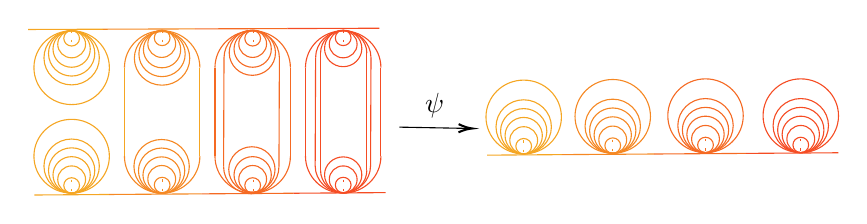
\begin{tikzpicture}[x=0.45pt,y=0.45pt,yscale=-1,xscale=1]
%uncomment if require: \path (0,330); %set diagram left start at 0, and has height of 330

%Shape: Ellipse [id:dp755042607694153] 
\draw  [color={rgb, 255:red, 245; green, 166; blue, 35 }  ,draw opacity=1 ] (28.58,172.86) .. controls (28.58,156.5) and (42.14,143.24) .. (58.86,143.24) .. controls (75.59,143.24) and (89.15,156.5) .. (89.15,172.86) .. controls (89.15,189.23) and (75.59,202.49) .. (58.86,202.49) .. controls (42.14,202.49) and (28.58,189.23) .. (28.58,172.86) -- cycle ;
%Shape: Ellipse [id:dp8592507789171753] 
\draw  [color={rgb, 255:red, 245; green, 166; blue, 35 }  ,draw opacity=1 ] (28.58,101.76) .. controls (28.58,85.4) and (42.14,72.13) .. (58.86,72.13) .. controls (75.59,72.13) and (89.15,85.4) .. (89.15,101.76) .. controls (89.15,118.12) and (75.59,131.39) .. (58.86,131.39) .. controls (42.14,131.39) and (28.58,118.12) .. (28.58,101.76) -- cycle ;
%Shape: Arc [id:dp5575659847483159] 
\draw  [draw opacity=0] (101.26,101.76) .. controls (101.26,101.76) and (101.26,101.76) .. (101.26,101.76) .. controls (101.26,85.4) and (114.82,72.13) .. (131.55,72.13) .. controls (148.27,72.13) and (161.83,85.4) .. (161.83,101.76) -- (131.55,101.76) -- cycle ; \draw  [color={rgb, 255:red, 245; green, 136; blue, 35 }  ,draw opacity=1 ] (101.26,101.76) .. controls (101.26,101.76) and (101.26,101.76) .. (101.26,101.76) .. controls (101.26,85.4) and (114.82,72.13) .. (131.55,72.13) .. controls (148.27,72.13) and (161.83,85.4) .. (161.83,101.76) ;  
%Shape: Arc [id:dp7393184648450104] 
\draw  [draw opacity=0] (161.83,172.86) .. controls (161.83,172.86) and (161.83,172.86) .. (161.83,172.86) .. controls (161.83,172.86) and (161.83,172.86) .. (161.83,172.86) .. controls (161.83,189.23) and (148.27,202.49) .. (131.55,202.49) .. controls (114.82,202.49) and (101.26,189.23) .. (101.26,172.86) -- (131.55,172.86) -- cycle ; \draw  [color={rgb, 255:red, 245; green, 136; blue, 35 }  ,draw opacity=1 ] (161.83,172.86) .. controls (161.83,172.86) and (161.83,172.86) .. (161.83,172.86) .. controls (161.83,172.86) and (161.83,172.86) .. (161.83,172.86) .. controls (161.83,189.23) and (148.27,202.49) .. (131.55,202.49) .. controls (114.82,202.49) and (101.26,189.23) .. (101.26,172.86) ;  
%Straight Lines [id:da6912455869646965] 
\draw [color={rgb, 255:red, 245; green, 166; blue, 35 }  ,draw opacity=1 ]   (101.26,101.76) -- (101.26,172.86) ;
%Straight Lines [id:da7415674220693267] 
\draw [color={rgb, 255:red, 245; green, 166; blue, 35 }  ,draw opacity=1 ]   (161.83,101.76) -- (161.83,172.86) ;
%Shape: Arc [id:dp2844251535638781] 
\draw  [draw opacity=0] (173.95,101.76) .. controls (173.95,101.76) and (173.95,101.76) .. (173.95,101.76) .. controls (173.95,85.4) and (187.51,72.13) .. (204.23,72.13) .. controls (220.96,72.13) and (234.52,85.4) .. (234.52,101.76) -- (204.23,101.76) -- cycle ; \draw  [color={rgb, 255:red, 245; green, 106; blue, 35 }  ,draw opacity=1 ] (173.95,101.76) .. controls (173.95,101.76) and (173.95,101.76) .. (173.95,101.76) .. controls (173.95,85.4) and (187.51,72.13) .. (204.23,72.13) .. controls (220.96,72.13) and (234.52,85.4) .. (234.52,101.76) ;  
%Shape: Arc [id:dp07026080518879607] 
\draw  [draw opacity=0] (234.52,172.86) .. controls (234.52,172.86) and (234.52,172.86) .. (234.52,172.86) .. controls (234.52,189.23) and (220.96,202.49) .. (204.23,202.49) .. controls (187.51,202.49) and (173.95,189.23) .. (173.95,172.86) -- (204.23,172.86) -- cycle ; \draw  [color={rgb, 255:red, 245; green, 106; blue, 35 }  ,draw opacity=1 ] (234.52,172.86) .. controls (234.52,172.86) and (234.52,172.86) .. (234.52,172.86) .. controls (234.52,189.23) and (220.96,202.49) .. (204.23,202.49) .. controls (187.51,202.49) and (173.95,189.23) .. (173.95,172.86) ;  
%Straight Lines [id:da4228728984431098] 
\draw [color={rgb, 255:red, 245; green, 106; blue, 35 }  ,draw opacity=1 ]   (173.95,101.76) -- (173.95,172.86) ;
%Straight Lines [id:da010401618689007575] 
\draw [color={rgb, 255:red, 245; green, 106; blue, 35 }  ,draw opacity=1 ]   (234.52,101.76) -- (234.52,172.86) ;
%Shape: Arc [id:dp5665130655467749] 
\draw  [draw opacity=0] (246.63,101.76) .. controls (246.63,101.76) and (246.63,101.76) .. (246.63,101.76) .. controls (246.63,85.4) and (260.19,72.13) .. (276.92,72.13) .. controls (293.64,72.13) and (307.2,85.4) .. (307.2,101.76) .. controls (307.2,101.76) and (307.2,101.76) .. (307.2,101.76) -- (276.92,101.76) -- cycle ; \draw  [color={rgb, 255:red, 245; green, 76; blue, 35 }  ,draw opacity=1 ] (246.63,101.76) .. controls (246.63,101.76) and (246.63,101.76) .. (246.63,101.76) .. controls (246.63,85.4) and (260.19,72.13) .. (276.92,72.13) .. controls (293.64,72.13) and (307.2,85.4) .. (307.2,101.76) .. controls (307.2,101.76) and (307.2,101.76) .. (307.2,101.76) ;  
%Shape: Arc [id:dp45839677289396485] 
\draw  [draw opacity=0] (307.2,172.86) .. controls (307.2,172.86) and (307.2,172.86) .. (307.2,172.86) .. controls (307.2,189.23) and (293.64,202.49) .. (276.92,202.49) .. controls (260.19,202.49) and (246.63,189.23) .. (246.63,172.86) .. controls (246.63,172.86) and (246.63,172.86) .. (246.63,172.86) -- (276.92,172.86) -- cycle ; \draw  [color={rgb, 255:red, 245; green, 76; blue, 35 }  ,draw opacity=1 ] (307.2,172.86) .. controls (307.2,172.86) and (307.2,172.86) .. (307.2,172.86) .. controls (307.2,189.23) and (293.64,202.49) .. (276.92,202.49) .. controls (260.19,202.49) and (246.63,189.23) .. (246.63,172.86) .. controls (246.63,172.86) and (246.63,172.86) .. (246.63,172.86) ;  
%Straight Lines [id:da9775394006068312] 
\draw [color={rgb, 255:red, 245; green, 76; blue, 35 }  ,draw opacity=1 ]   (246.63,101.76) -- (246.63,172.86) ;
%Straight Lines [id:da8522804711696934] 
\draw [color={rgb, 255:red, 245; green, 76; blue, 35 }  ,draw opacity=1 ]   (307.2,101.76) -- (307.2,172.86) ;
%Shape: Ellipse [id:dp7061775084823935] 
\draw  [color={rgb, 255:red, 245; green, 136; blue, 35 }  ,draw opacity=1 ] (109.22,94.2) .. controls (109.22,82.26) and (119.18,72.57) .. (131.46,72.57) .. controls (143.74,72.57) and (153.7,82.26) .. (153.7,94.2) .. controls (153.7,106.14) and (143.74,115.82) .. (131.46,115.82) .. controls (119.18,115.82) and (109.22,106.14) .. (109.22,94.2) -- cycle ;
%Shape: Ellipse [id:dp18615492139699985] 
\draw  [color={rgb, 255:red, 245; green, 136; blue, 35 }  ,draw opacity=1 ] (108.88,181.04) .. controls (108.88,169.09) and (118.83,159.41) .. (131.11,159.41) .. controls (143.4,159.41) and (153.35,169.09) .. (153.35,181.04) .. controls (153.35,192.98) and (143.4,202.66) .. (131.11,202.66) .. controls (118.83,202.66) and (108.88,192.98) .. (108.88,181.04) -- cycle ;
%Shape: Arc [id:dp8538635445684597] 
\draw  [draw opacity=0] (181.21,93.89) .. controls (181.21,81.87) and (191.17,72.13) .. (203.45,72.13) .. controls (215.73,72.13) and (225.69,81.87) .. (225.69,93.89) -- (203.45,93.89) -- cycle ; \draw  [color={rgb, 255:red, 245; green, 106; blue, 35 }  ,draw opacity=1 ] (181.21,93.89) .. controls (181.21,81.87) and (191.17,72.13) .. (203.45,72.13) .. controls (215.73,72.13) and (225.69,81.87) .. (225.69,93.89) ;  
%Shape: Arc [id:dp49810715044832066] 
\draw  [draw opacity=0] (225.34,181.24) .. controls (225.34,193.26) and (215.39,203) .. (203.11,203) .. controls (190.82,203) and (180.87,193.26) .. (180.87,181.24) -- (203.11,181.24) -- cycle ; \draw  [color={rgb, 255:red, 245; green, 106; blue, 35 }  ,draw opacity=1 ] (225.34,181.24) .. controls (225.34,193.26) and (215.39,203) .. (203.11,203) .. controls (190.82,203) and (180.87,193.26) .. (180.87,181.24) ;  
%Straight Lines [id:da06818006829326317] 
\draw [color={rgb, 255:red, 245; green, 106; blue, 35 }  ,draw opacity=1 ]   (181.21,93.89) -- (180.87,181.24) ;
%Straight Lines [id:da9641952746953396] 
\draw [color={rgb, 255:red, 245; green, 106; blue, 35 }  ,draw opacity=1 ]   (225.69,93.89) -- (225.34,181.24) ;

%Shape: Arc [id:dp5750096331920825] 
\draw  [draw opacity=0] (254.76,93.74) .. controls (254.76,81.81) and (264.72,72.13) .. (277,72.13) .. controls (289.28,72.13) and (299.24,81.81) .. (299.24,93.74) -- (277,93.74) -- cycle ; \draw  [color={rgb, 255:red, 245; green, 76; blue, 35 }  ,draw opacity=1 ] (254.76,93.74) .. controls (254.76,81.81) and (264.72,72.13) .. (277,72.13) .. controls (289.28,72.13) and (299.24,81.81) .. (299.24,93.74) ;  
%Shape: Arc [id:dp4452867146415097] 
\draw  [draw opacity=0] (298.89,180.54) .. controls (298.89,192.48) and (288.94,202.15) .. (276.66,202.15) .. controls (264.37,202.15) and (254.42,192.48) .. (254.42,180.54) -- (276.66,180.54) -- cycle ; \draw  [color={rgb, 255:red, 245; green, 76; blue, 35 }  ,draw opacity=1 ] (298.89,180.54) .. controls (298.89,192.48) and (288.94,202.15) .. (276.66,202.15) .. controls (264.37,202.15) and (254.42,192.48) .. (254.42,180.54) ;  
%Straight Lines [id:da47654812565410376] 
\draw [color={rgb, 255:red, 245; green, 76; blue, 35 }  ,draw opacity=1 ]   (254.76,93.74) -- (254.42,180.54) ;
%Straight Lines [id:da3541247537262896] 
\draw [color={rgb, 255:red, 245; green, 76; blue, 35 }  ,draw opacity=1 ]   (299.24,93.74) -- (298.89,180.54) ;

%Shape: Ellipse [id:dp015112826866313211] 
\draw  [color={rgb, 255:red, 245; green, 166; blue, 35 }  ,draw opacity=1 ] (36.63,93.85) .. controls (36.63,81.86) and (46.58,72.13) .. (58.86,72.13) .. controls (71.14,72.13) and (81.1,81.86) .. (81.1,93.85) .. controls (81.1,105.85) and (71.14,115.58) .. (58.86,115.58) .. controls (46.58,115.58) and (36.63,105.85) .. (36.63,93.85) -- cycle ;
%Shape: Ellipse [id:dp08480110306864375] 
\draw  [color={rgb, 255:red, 245; green, 166; blue, 35 }  ,draw opacity=1 ] (36.63,180.77) .. controls (36.63,168.77) and (46.58,159.05) .. (58.86,159.05) .. controls (71.14,159.05) and (81.1,168.77) .. (81.1,180.77) .. controls (81.1,192.77) and (71.14,202.49) .. (58.86,202.49) .. controls (46.58,202.49) and (36.63,192.77) .. (36.63,180.77) -- cycle ;
%Shape: Ellipse [id:dp6396517846512791] 
\draw  [color={rgb, 255:red, 245; green, 166; blue, 35 }  ,draw opacity=1 ] (40.28,90.31) .. controls (40.28,80.27) and (48.6,72.13) .. (58.86,72.13) .. controls (69.13,72.13) and (77.45,80.27) .. (77.45,90.31) .. controls (77.45,100.36) and (69.13,108.5) .. (58.86,108.5) .. controls (48.6,108.5) and (40.28,100.36) .. (40.28,90.31) -- cycle ;
%Shape: Ellipse [id:dp26863757459073234] 
\draw  [color={rgb, 255:red, 245; green, 166; blue, 35 }  ,draw opacity=1 ] (40.28,184.31) .. controls (40.28,174.27) and (48.6,166.12) .. (58.86,166.12) .. controls (69.13,166.12) and (77.45,174.27) .. (77.45,184.31) .. controls (77.45,194.35) and (69.13,202.49) .. (58.86,202.49) .. controls (48.6,202.49) and (40.28,194.35) .. (40.28,184.31) -- cycle ;
%Shape: Ellipse [id:dp6888221898815015] 
\draw  [color={rgb, 255:red, 245; green, 136; blue, 35 }  ,draw opacity=1 ] (112.87,90.76) .. controls (112.87,80.72) and (121.19,72.57) .. (131.46,72.57) .. controls (141.73,72.57) and (150.05,80.72) .. (150.05,90.76) .. controls (150.05,100.8) and (141.73,108.94) .. (131.46,108.94) .. controls (121.19,108.94) and (112.87,100.8) .. (112.87,90.76) -- cycle ;
%Shape: Ellipse [id:dp6131335458949229] 
\draw  [color={rgb, 255:red, 245; green, 136; blue, 35 }  ,draw opacity=1 ] (112.53,184.48) .. controls (112.53,174.43) and (120.85,166.29) .. (131.11,166.29) .. controls (141.38,166.29) and (149.7,174.43) .. (149.7,184.48) .. controls (149.7,194.52) and (141.38,202.66) .. (131.11,202.66) .. controls (120.85,202.66) and (112.53,194.52) .. (112.53,184.48) -- cycle ;
%Shape: Arc [id:dp06200106763647828] 
\draw  [draw opacity=0] (258.73,90.12) .. controls (258.73,90.12) and (258.73,90.12) .. (258.73,90.12) .. controls (258.73,80.07) and (267.05,71.93) .. (277.32,71.93) .. controls (287.58,71.93) and (295.91,80.07) .. (295.91,90.12) -- (277.32,90.12) -- cycle ; \draw  [color={rgb, 255:red, 245; green, 76; blue, 35 }  ,draw opacity=1 ] (258.73,90.12) .. controls (258.73,90.12) and (258.73,90.12) .. (258.73,90.12) .. controls (258.73,80.07) and (267.05,71.93) .. (277.32,71.93) .. controls (287.58,71.93) and (295.91,80.07) .. (295.91,90.12) ;  
%Shape: Arc [id:dp5244952406542043] 
\draw  [draw opacity=0] (295.91,184.11) .. controls (295.91,184.11) and (295.91,184.11) .. (295.91,184.11) .. controls (295.91,184.11) and (295.91,184.11) .. (295.91,184.11) .. controls (295.91,194.15) and (287.58,202.29) .. (277.32,202.29) .. controls (267.05,202.29) and (258.73,194.15) .. (258.73,184.11) -- (277.32,184.11) -- cycle ; \draw  [color={rgb, 255:red, 245; green, 76; blue, 35 }  ,draw opacity=1 ] (295.91,184.11) .. controls (295.91,184.11) and (295.91,184.11) .. (295.91,184.11) .. controls (295.91,184.11) and (295.91,184.11) .. (295.91,184.11) .. controls (295.91,194.15) and (287.58,202.29) .. (277.32,202.29) .. controls (267.05,202.29) and (258.73,194.15) .. (258.73,184.11) ;  
%Straight Lines [id:da7525466584384344] 
\draw [color={rgb, 255:red, 245; green, 76; blue, 35 }  ,draw opacity=1 ]   (258.73,90.12) -- (258.73,184.11) ;
%Straight Lines [id:da25122929214675105] 
\draw [color={rgb, 255:red, 245; green, 76; blue, 35 }  ,draw opacity=1 ]   (295.91,90.31) -- (295.91,184.31) ;

%Shape: Ellipse [id:dp9916809302488827] 
\draw  [color={rgb, 255:red, 245; green, 166; blue, 35 }  ,draw opacity=1 ] (43.89,86.77) .. controls (43.89,78.69) and (50.6,72.13) .. (58.86,72.13) .. controls (67.13,72.13) and (73.83,78.69) .. (73.83,86.77) .. controls (73.83,94.86) and (67.13,101.42) .. (58.86,101.42) .. controls (50.6,101.42) and (43.89,94.86) .. (43.89,86.77) -- cycle ;
%Shape: Ellipse [id:dp21228108456554207] 
\draw  [color={rgb, 255:red, 245; green, 166; blue, 35 }  ,draw opacity=1 ] (43.89,187.85) .. controls (43.89,179.76) and (50.6,173.2) .. (58.86,173.2) .. controls (67.13,173.2) and (73.83,179.76) .. (73.83,187.85) .. controls (73.83,195.94) and (67.13,202.49) .. (58.86,202.49) .. controls (50.6,202.49) and (43.89,195.94) .. (43.89,187.85) -- cycle ;
%Shape: Ellipse [id:dp08651193901107368] 
\draw  [color={rgb, 255:red, 245; green, 136; blue, 35 }  ,draw opacity=1 ] (116.49,87.22) .. controls (116.49,79.13) and (123.19,72.57) .. (131.46,72.57) .. controls (139.73,72.57) and (146.43,79.13) .. (146.43,87.22) .. controls (146.43,95.31) and (139.73,101.86) .. (131.46,101.86) .. controls (123.19,101.86) and (116.49,95.31) .. (116.49,87.22) -- cycle ;
%Shape: Ellipse [id:dp6967140272448221] 
\draw  [color={rgb, 255:red, 245; green, 136; blue, 35 }  ,draw opacity=1 ] (116.14,188.02) .. controls (116.14,179.93) and (122.85,173.37) .. (131.11,173.37) .. controls (139.38,173.37) and (146.08,179.93) .. (146.08,188.02) .. controls (146.08,196.1) and (139.38,202.66) .. (131.11,202.66) .. controls (122.85,202.66) and (116.14,196.1) .. (116.14,188.02) -- cycle ;
%Shape: Ellipse [id:dp3442874649468213] 
\draw  [color={rgb, 255:red, 245; green, 106; blue, 35 }  ,draw opacity=1 ] (189.26,86.77) .. controls (189.26,78.69) and (195.96,72.13) .. (204.23,72.13) .. controls (212.5,72.13) and (219.2,78.69) .. (219.2,86.77) .. controls (219.2,94.86) and (212.5,101.42) .. (204.23,101.42) .. controls (195.96,101.42) and (189.26,94.86) .. (189.26,86.77) -- cycle ;
%Shape: Ellipse [id:dp04347435390523402] 
\draw  [color={rgb, 255:red, 245; green, 106; blue, 35 }  ,draw opacity=1 ] (189.26,187.85) .. controls (189.26,179.76) and (195.96,173.2) .. (204.23,173.2) .. controls (212.5,173.2) and (219.2,179.76) .. (219.2,187.85) .. controls (219.2,195.94) and (212.5,202.49) .. (204.23,202.49) .. controls (195.96,202.49) and (189.26,195.94) .. (189.26,187.85) -- cycle ;
%Shape: Ellipse [id:dp26123086484050506] 
\draw  [color={rgb, 255:red, 245; green, 166; blue, 35 }  ,draw opacity=1 ] (47.7,82.93) .. controls (47.7,76.9) and (52.7,72.01) .. (58.86,72.01) .. controls (65.03,72.01) and (70.03,76.9) .. (70.03,82.93) .. controls (70.03,88.96) and (65.03,93.85) .. (58.86,93.85) .. controls (52.7,93.85) and (47.7,88.96) .. (47.7,82.93) -- cycle ;
%Shape: Ellipse [id:dp09091362212598297] 
\draw  [color={rgb, 255:red, 245; green, 166; blue, 35 }  ,draw opacity=1 ] (47.7,191.57) .. controls (47.7,185.54) and (52.7,180.65) .. (58.86,180.65) .. controls (65.03,180.65) and (70.03,185.54) .. (70.03,191.57) .. controls (70.03,197.6) and (65.03,202.49) .. (58.86,202.49) .. controls (52.7,202.49) and (47.7,197.6) .. (47.7,191.57) -- cycle ;
%Shape: Ellipse [id:dp3767844311743297] 
\draw  [color={rgb, 255:red, 245; green, 136; blue, 35 }  ,draw opacity=1 ] (120.04,82.6) .. controls (120.04,76.56) and (125.04,71.68) .. (131.2,71.68) .. controls (137.37,71.68) and (142.36,76.56) .. (142.36,82.6) .. controls (142.36,88.63) and (137.37,93.52) .. (131.2,93.52) .. controls (125.04,93.52) and (120.04,88.63) .. (120.04,82.6) -- cycle ;
%Shape: Ellipse [id:dp03544985956989655] 
\draw  [color={rgb, 255:red, 245; green, 136; blue, 35 }  ,draw opacity=1 ] (120.04,191.23) .. controls (120.04,185.2) and (125.04,180.31) .. (131.2,180.31) .. controls (137.37,180.31) and (142.36,185.2) .. (142.36,191.23) .. controls (142.36,197.26) and (137.37,202.15) .. (131.2,202.15) .. controls (125.04,202.15) and (120.04,197.26) .. (120.04,191.23) -- cycle ;
%Shape: Ellipse [id:dp06917760052791733] 
\draw  [color={rgb, 255:red, 245; green, 106; blue, 35 }  ,draw opacity=1 ] (193.07,82.6) .. controls (193.07,76.56) and (198.07,71.68) .. (204.23,71.68) .. controls (210.4,71.68) and (215.39,76.56) .. (215.39,82.6) .. controls (215.39,88.63) and (210.4,93.52) .. (204.23,93.52) .. controls (198.07,93.52) and (193.07,88.63) .. (193.07,82.6) -- cycle ;
%Shape: Ellipse [id:dp9282575291068949] 
\draw  [color={rgb, 255:red, 245; green, 106; blue, 35 }  ,draw opacity=1 ] (193.07,191.23) .. controls (193.07,185.2) and (198.07,180.31) .. (204.23,180.31) .. controls (210.4,180.31) and (215.39,185.2) .. (215.39,191.23) .. controls (215.39,197.26) and (210.4,202.15) .. (204.23,202.15) .. controls (198.07,202.15) and (193.07,197.26) .. (193.07,191.23) -- cycle ;
%Shape: Ellipse [id:dp07195796370829588] 
\draw  [color={rgb, 255:red, 245; green, 76; blue, 35 }  ,draw opacity=1 ] (265.75,82.93) .. controls (265.75,76.9) and (270.75,72.01) .. (276.92,72.01) .. controls (283.08,72.01) and (288.08,76.9) .. (288.08,82.93) .. controls (288.08,88.96) and (283.08,93.85) .. (276.92,93.85) .. controls (270.75,93.85) and (265.75,88.96) .. (265.75,82.93) -- cycle ;
%Shape: Ellipse [id:dp5724266197209639] 
\draw  [color={rgb, 255:red, 245; green, 76; blue, 35 }  ,draw opacity=1 ] (265.75,191.57) .. controls (265.75,185.54) and (270.75,180.65) .. (276.92,180.65) .. controls (283.08,180.65) and (288.08,185.54) .. (288.08,191.57) .. controls (288.08,197.6) and (283.08,202.49) .. (276.92,202.49) .. controls (270.75,202.49) and (265.75,197.6) .. (265.75,191.57) -- cycle ;
%Shape: Ellipse [id:dp5350672711499449] 
\draw  [color={rgb, 255:red, 245; green, 166; blue, 35 }  ,draw opacity=1 ] (52.55,78.19) .. controls (52.55,74.78) and (55.37,72.01) .. (58.86,72.01) .. controls (62.35,72.01) and (65.18,74.78) .. (65.18,78.19) .. controls (65.18,81.61) and (62.35,84.37) .. (58.86,84.37) .. controls (55.37,84.37) and (52.55,81.61) .. (52.55,78.19) -- cycle ;
%Shape: Ellipse [id:dp44217018518301565] 
\draw  [color={rgb, 255:red, 245; green, 166; blue, 35 }  ,draw opacity=1 ] (52.55,196.31) .. controls (52.55,192.9) and (55.37,190.13) .. (58.86,190.13) .. controls (62.35,190.13) and (65.18,192.9) .. (65.18,196.31) .. controls (65.18,199.73) and (62.35,202.49) .. (58.86,202.49) .. controls (55.37,202.49) and (52.55,199.73) .. (52.55,196.31) -- cycle ;
%Shape: Ellipse [id:dp2098277175532065] 
\draw  [color={rgb, 255:red, 245; green, 136; blue, 35 }  ,draw opacity=1 ] (125.23,77.85) .. controls (125.23,74.44) and (128.06,71.68) .. (131.55,71.68) .. controls (135.04,71.68) and (137.86,74.44) .. (137.86,77.85) .. controls (137.86,81.27) and (135.04,84.03) .. (131.55,84.03) .. controls (128.06,84.03) and (125.23,81.27) .. (125.23,77.85) -- cycle ;
%Shape: Ellipse [id:dp8563776640680607] 
\draw  [color={rgb, 255:red, 245; green, 136; blue, 35 }  ,draw opacity=1 ] (125.23,195.97) .. controls (125.23,192.56) and (128.06,189.79) .. (131.55,189.79) .. controls (135.04,189.79) and (137.86,192.56) .. (137.86,195.97) .. controls (137.86,199.39) and (135.04,202.15) .. (131.55,202.15) .. controls (128.06,202.15) and (125.23,199.39) .. (125.23,195.97) -- cycle ;
%Shape: Ellipse [id:dp17239593316849888] 
\draw  [color={rgb, 255:red, 245; green, 106; blue, 35 }  ,draw opacity=1 ] (197.91,78.19) .. controls (197.91,74.78) and (200.74,72.01) .. (204.23,72.01) .. controls (207.72,72.01) and (210.55,74.78) .. (210.55,78.19) .. controls (210.55,81.61) and (207.72,84.37) .. (204.23,84.37) .. controls (200.74,84.37) and (197.91,81.61) .. (197.91,78.19) -- cycle ;
%Shape: Ellipse [id:dp9221214438967847] 
\draw  [color={rgb, 255:red, 245; green, 106; blue, 35 }  ,draw opacity=1 ] (197.91,196.31) .. controls (197.91,192.9) and (200.74,190.13) .. (204.23,190.13) .. controls (207.72,190.13) and (210.55,192.9) .. (210.55,196.31) .. controls (210.55,199.73) and (207.72,202.49) .. (204.23,202.49) .. controls (200.74,202.49) and (197.91,199.73) .. (197.91,196.31) -- cycle ;
%Shape: Ellipse [id:dp7717878656733393] 
\draw  [color={rgb, 255:red, 245; green, 76; blue, 35 }  ,draw opacity=1 ] (270.6,77.85) .. controls (270.6,74.44) and (273.43,71.68) .. (276.92,71.68) .. controls (280.4,71.68) and (283.23,74.44) .. (283.23,77.85) .. controls (283.23,81.27) and (280.4,84.03) .. (276.92,84.03) .. controls (273.43,84.03) and (270.6,81.27) .. (270.6,77.85) -- cycle ;
%Shape: Ellipse [id:dp023181803110648436] 
\draw  [color={rgb, 255:red, 245; green, 76; blue, 35 }  ,draw opacity=1 ] (270.6,195.97) .. controls (270.6,192.56) and (273.43,189.79) .. (276.92,189.79) .. controls (280.4,189.79) and (283.23,192.56) .. (283.23,195.97) .. controls (283.23,199.39) and (280.4,202.15) .. (276.92,202.15) .. controls (273.43,202.15) and (270.6,199.39) .. (270.6,195.97) -- cycle ;
%Straight Lines [id:da3971902588574284] 
\draw [color={rgb, 255:red, 245; green, 166; blue, 35 }  ,draw opacity=1 ] [dash pattern={on 0.84pt off 2.51pt}]  (58.86,72.01) -- (58.86,82.93) ;
%Straight Lines [id:da42843264406748816] 
\draw [color={rgb, 255:red, 245; green, 166; blue, 35 }  ,draw opacity=1 ] [dash pattern={on 0.84pt off 2.51pt}]  (58.86,191.57) -- (58.86,202.49) ;
%Straight Lines [id:da37965867604678805] 
\draw [color={rgb, 255:red, 245; green, 136; blue, 35 }  ,draw opacity=1 ] [dash pattern={on 0.84pt off 2.51pt}]  (131.85,71.79) -- (131.85,82.71) ;
%Straight Lines [id:da46421804971724734] 
\draw [color={rgb, 255:red, 245; green, 136; blue, 35 }  ,draw opacity=1 ] [dash pattern={on 0.84pt off 2.51pt}]  (131.85,191.35) -- (131.85,202.27) ;
%Straight Lines [id:da38984619285948274] 
\draw [color={rgb, 255:red, 245; green, 106; blue, 35 }  ,draw opacity=1 ] [dash pattern={on 0.84pt off 2.51pt}]  (204.55,72.08) -- (204.55,83) ;
%Straight Lines [id:da16765663625080263] 
\draw [color={rgb, 255:red, 245; green, 106; blue, 35 }  ,draw opacity=1 ] [dash pattern={on 0.84pt off 2.51pt}]  (204.55,191.64) -- (204.55,202.56) ;
%Straight Lines [id:da1739151256946022] 
\draw [color={rgb, 255:red, 245; green, 76; blue, 35 }  ,draw opacity=1 ] [dash pattern={on 0.84pt off 2.51pt}]  (277.24,72.08) -- (277.24,83) ;
%Straight Lines [id:da30219095449842914] 
\draw [color={rgb, 255:red, 245; green, 76; blue, 35 }  ,draw opacity=1 ] [dash pattern={on 0.84pt off 2.51pt}]  (277.24,191.64) -- (277.24,202.56) ;
%Shape: Ellipse [id:dp918610407888359] 
\draw  [color={rgb, 255:red, 245; green, 106; blue, 35 }  ,draw opacity=1 ] (185.38,89.73) .. controls (185.38,79.69) and (193.7,71.55) .. (203.96,71.55) .. controls (214.23,71.55) and (222.55,79.69) .. (222.55,89.73) .. controls (222.55,99.77) and (214.23,107.91) .. (203.96,107.91) .. controls (193.7,107.91) and (185.38,99.77) .. (185.38,89.73) -- cycle ;
%Shape: Ellipse [id:dp5036168348216472] 
\draw  [color={rgb, 255:red, 245; green, 106; blue, 35 }  ,draw opacity=1 ] (185.03,183.45) .. controls (185.03,173.41) and (193.35,165.26) .. (203.62,165.26) .. controls (213.88,165.26) and (222.2,173.41) .. (222.2,183.45) .. controls (222.2,193.49) and (213.88,201.63) .. (203.62,201.63) .. controls (193.35,201.63) and (185.03,193.49) .. (185.03,183.45) -- cycle ;
%Shape: Ellipse [id:dp2915912012548635] 
\draw  [color={rgb, 255:red, 245; green, 76; blue, 35 }  ,draw opacity=1 ] (261.95,86.32) .. controls (261.95,78.23) and (268.65,71.68) .. (276.92,71.68) .. controls (285.18,71.68) and (291.88,78.23) .. (291.88,86.32) .. controls (291.88,94.41) and (285.18,100.96) .. (276.92,100.96) .. controls (268.65,100.96) and (261.95,94.41) .. (261.95,86.32) -- cycle ;
%Shape: Ellipse [id:dp1895258307785581] 
\draw  [color={rgb, 255:red, 245; green, 76; blue, 35 }  ,draw opacity=1 ] (261.95,187.77) .. controls (261.95,179.83) and (268.65,173.39) .. (276.92,173.39) .. controls (285.18,173.39) and (291.88,179.83) .. (291.88,187.77) .. controls (291.88,195.71) and (285.18,202.15) .. (276.92,202.15) .. controls (268.65,202.15) and (261.95,195.71) .. (261.95,187.77) -- cycle ;
%Shape: Ellipse [id:dp1731328879855092] 
\draw  [color={rgb, 255:red, 245; green, 166; blue, 35 }  ,draw opacity=1 ] (391.58,141.36) .. controls (391.58,125) and (405.14,111.74) .. (421.86,111.74) .. controls (438.59,111.74) and (452.15,125) .. (452.15,141.36) .. controls (452.15,157.73) and (438.59,170.99) .. (421.86,170.99) .. controls (405.14,170.99) and (391.58,157.73) .. (391.58,141.36) -- cycle ;
%Shape: Ellipse [id:dp9732378329313575] 
\draw  [color={rgb, 255:red, 245; green, 166; blue, 35 }  ,draw opacity=1 ] (399.63,149.27) .. controls (399.63,137.27) and (409.58,127.55) .. (421.86,127.55) .. controls (434.14,127.55) and (444.1,137.27) .. (444.1,149.27) .. controls (444.1,161.27) and (434.14,170.99) .. (421.86,170.99) .. controls (409.58,170.99) and (399.63,161.27) .. (399.63,149.27) -- cycle ;
%Shape: Ellipse [id:dp9413816540100547] 
\draw  [color={rgb, 255:red, 245; green, 166; blue, 35 }  ,draw opacity=1 ] (403.28,152.81) .. controls (403.28,142.77) and (411.6,134.62) .. (421.86,134.62) .. controls (432.13,134.62) and (440.45,142.77) .. (440.45,152.81) .. controls (440.45,162.85) and (432.13,170.99) .. (421.86,170.99) .. controls (411.6,170.99) and (403.28,162.85) .. (403.28,152.81) -- cycle ;
%Shape: Ellipse [id:dp30124762171913044] 
\draw  [color={rgb, 255:red, 245; green, 166; blue, 35 }  ,draw opacity=1 ] (406.89,156.35) .. controls (406.89,148.26) and (413.6,141.7) .. (421.86,141.7) .. controls (430.13,141.7) and (436.83,148.26) .. (436.83,156.35) .. controls (436.83,164.44) and (430.13,170.99) .. (421.86,170.99) .. controls (413.6,170.99) and (406.89,164.44) .. (406.89,156.35) -- cycle ;
%Shape: Ellipse [id:dp9690150665096517] 
\draw  [color={rgb, 255:red, 245; green, 166; blue, 35 }  ,draw opacity=1 ] (410.7,160.07) .. controls (410.7,154.04) and (415.7,149.15) .. (421.86,149.15) .. controls (428.03,149.15) and (433.03,154.04) .. (433.03,160.07) .. controls (433.03,166.1) and (428.03,170.99) .. (421.86,170.99) .. controls (415.7,170.99) and (410.7,166.1) .. (410.7,160.07) -- cycle ;
%Shape: Ellipse [id:dp47159558579377203] 
\draw  [color={rgb, 255:red, 245; green, 166; blue, 35 }  ,draw opacity=1 ] (415.55,164.81) .. controls (415.55,161.4) and (418.37,158.63) .. (421.86,158.63) .. controls (425.35,158.63) and (428.18,161.4) .. (428.18,164.81) .. controls (428.18,168.23) and (425.35,170.99) .. (421.86,170.99) .. controls (418.37,170.99) and (415.55,168.23) .. (415.55,164.81) -- cycle ;
%Straight Lines [id:da9068595717993126] 
\draw [color={rgb, 255:red, 245; green, 166; blue, 35 }  ,draw opacity=1 ] [dash pattern={on 0.84pt off 2.51pt}]  (421.86,160.07) -- (421.86,170.99) ;
%Shape: Ellipse [id:dp9481609733703893] 
\draw  [color={rgb, 255:red, 245; green, 136; blue, 35 }  ,draw opacity=1 ] (463.08,140.86) .. controls (463.08,124.5) and (476.64,111.24) .. (493.36,111.24) .. controls (510.09,111.24) and (523.65,124.5) .. (523.65,140.86) .. controls (523.65,157.23) and (510.09,170.49) .. (493.36,170.49) .. controls (476.64,170.49) and (463.08,157.23) .. (463.08,140.86) -- cycle ;
%Shape: Ellipse [id:dp12137927666296189] 
\draw  [color={rgb, 255:red, 245; green, 136; blue, 35 }  ,draw opacity=1 ] (471.13,148.77) .. controls (471.13,136.77) and (481.08,127.05) .. (493.36,127.05) .. controls (505.64,127.05) and (515.6,136.77) .. (515.6,148.77) .. controls (515.6,160.77) and (505.64,170.49) .. (493.36,170.49) .. controls (481.08,170.49) and (471.13,160.77) .. (471.13,148.77) -- cycle ;
%Shape: Ellipse [id:dp947697804041952] 
\draw  [color={rgb, 255:red, 245; green, 136; blue, 35 }  ,draw opacity=1 ] (474.78,152.31) .. controls (474.78,142.27) and (483.1,134.12) .. (493.36,134.12) .. controls (503.63,134.12) and (511.95,142.27) .. (511.95,152.31) .. controls (511.95,162.35) and (503.63,170.49) .. (493.36,170.49) .. controls (483.1,170.49) and (474.78,162.35) .. (474.78,152.31) -- cycle ;
%Shape: Ellipse [id:dp5047542192896263] 
\draw  [color={rgb, 255:red, 245; green, 136; blue, 35 }  ,draw opacity=1 ] (478.39,155.85) .. controls (478.39,147.76) and (485.1,141.2) .. (493.36,141.2) .. controls (501.63,141.2) and (508.33,147.76) .. (508.33,155.85) .. controls (508.33,163.94) and (501.63,170.49) .. (493.36,170.49) .. controls (485.1,170.49) and (478.39,163.94) .. (478.39,155.85) -- cycle ;
%Shape: Ellipse [id:dp1694890660895435] 
\draw  [color={rgb, 255:red, 245; green, 136; blue, 35 }  ,draw opacity=1 ] (482.2,159.57) .. controls (482.2,153.54) and (487.2,148.65) .. (493.36,148.65) .. controls (499.53,148.65) and (504.53,153.54) .. (504.53,159.57) .. controls (504.53,165.6) and (499.53,170.49) .. (493.36,170.49) .. controls (487.2,170.49) and (482.2,165.6) .. (482.2,159.57) -- cycle ;
%Shape: Ellipse [id:dp0158322262495747] 
\draw  [color={rgb, 255:red, 245; green, 136; blue, 35 }  ,draw opacity=1 ] (487.05,164.31) .. controls (487.05,160.9) and (489.87,158.13) .. (493.36,158.13) .. controls (496.85,158.13) and (499.68,160.9) .. (499.68,164.31) .. controls (499.68,167.73) and (496.85,170.49) .. (493.36,170.49) .. controls (489.87,170.49) and (487.05,167.73) .. (487.05,164.31) -- cycle ;
%Straight Lines [id:da4385836241002009] 
\draw [color={rgb, 255:red, 245; green, 136; blue, 35 }  ,draw opacity=1 ] [dash pattern={on 0.84pt off 2.51pt}]  (493.36,159.57) -- (493.36,170.49) ;
%Shape: Ellipse [id:dp28527268977190623] 
\draw  [color={rgb, 255:red, 245; green, 106; blue, 35 }  ,draw opacity=1 ] (537.58,140.36) .. controls (537.58,124) and (551.14,110.74) .. (567.86,110.74) .. controls (584.59,110.74) and (598.15,124) .. (598.15,140.36) .. controls (598.15,156.73) and (584.59,169.99) .. (567.86,169.99) .. controls (551.14,169.99) and (537.58,156.73) .. (537.58,140.36) -- cycle ;
%Shape: Ellipse [id:dp3998947516220763] 
\draw  [color={rgb, 255:red, 245; green, 106; blue, 35 }  ,draw opacity=1 ] (545.63,148.27) .. controls (545.63,136.27) and (555.58,126.55) .. (567.86,126.55) .. controls (580.14,126.55) and (590.1,136.27) .. (590.1,148.27) .. controls (590.1,160.27) and (580.14,169.99) .. (567.86,169.99) .. controls (555.58,169.99) and (545.63,160.27) .. (545.63,148.27) -- cycle ;
%Shape: Ellipse [id:dp8224189990558726] 
\draw  [color={rgb, 255:red, 245; green, 106; blue, 35 }  ,draw opacity=1 ] (549.28,151.81) .. controls (549.28,141.77) and (557.6,133.62) .. (567.86,133.62) .. controls (578.13,133.62) and (586.45,141.77) .. (586.45,151.81) .. controls (586.45,161.85) and (578.13,169.99) .. (567.86,169.99) .. controls (557.6,169.99) and (549.28,161.85) .. (549.28,151.81) -- cycle ;
%Shape: Ellipse [id:dp7344552633963315] 
\draw  [color={rgb, 255:red, 245; green, 106; blue, 35 }  ,draw opacity=1 ] (552.89,155.35) .. controls (552.89,147.26) and (559.6,140.7) .. (567.86,140.7) .. controls (576.13,140.7) and (582.83,147.26) .. (582.83,155.35) .. controls (582.83,163.44) and (576.13,169.99) .. (567.86,169.99) .. controls (559.6,169.99) and (552.89,163.44) .. (552.89,155.35) -- cycle ;
%Shape: Ellipse [id:dp3172805904520115] 
\draw  [color={rgb, 255:red, 245; green, 106; blue, 35 }  ,draw opacity=1 ] (556.7,159.07) .. controls (556.7,153.04) and (561.7,148.15) .. (567.86,148.15) .. controls (574.03,148.15) and (579.03,153.04) .. (579.03,159.07) .. controls (579.03,165.1) and (574.03,169.99) .. (567.86,169.99) .. controls (561.7,169.99) and (556.7,165.1) .. (556.7,159.07) -- cycle ;
%Shape: Ellipse [id:dp2529561367010139] 
\draw  [color={rgb, 255:red, 245; green, 106; blue, 35 }  ,draw opacity=1 ] (561.55,163.81) .. controls (561.55,160.4) and (564.37,157.63) .. (567.86,157.63) .. controls (571.35,157.63) and (574.18,160.4) .. (574.18,163.81) .. controls (574.18,167.23) and (571.35,169.99) .. (567.86,169.99) .. controls (564.37,169.99) and (561.55,167.23) .. (561.55,163.81) -- cycle ;
%Straight Lines [id:da4322407483680014] 
\draw [color={rgb, 255:red, 245; green, 106; blue, 35 }  ,draw opacity=1 ] [dash pattern={on 0.84pt off 2.51pt}]  (567.86,159.07) -- (567.86,169.99) ;
%Shape: Ellipse [id:dp005153834373483934] 
\draw  [color={rgb, 255:red, 245; green, 76; blue, 35 }  ,draw opacity=1 ] (614.08,140.36) .. controls (614.08,124) and (627.64,110.74) .. (644.36,110.74) .. controls (661.09,110.74) and (674.65,124) .. (674.65,140.36) .. controls (674.65,156.73) and (661.09,169.99) .. (644.36,169.99) .. controls (627.64,169.99) and (614.08,156.73) .. (614.08,140.36) -- cycle ;
%Shape: Ellipse [id:dp905688444123756] 
\draw  [color={rgb, 255:red, 245; green, 76; blue, 35 }  ,draw opacity=1 ] (622.13,148.27) .. controls (622.13,136.27) and (632.08,126.55) .. (644.36,126.55) .. controls (656.64,126.55) and (666.6,136.27) .. (666.6,148.27) .. controls (666.6,160.27) and (656.64,169.99) .. (644.36,169.99) .. controls (632.08,169.99) and (622.13,160.27) .. (622.13,148.27) -- cycle ;
%Shape: Ellipse [id:dp39318831006463884] 
\draw  [color={rgb, 255:red, 245; green, 76; blue, 35 }  ,draw opacity=1 ] (625.78,151.81) .. controls (625.78,141.77) and (634.1,133.62) .. (644.36,133.62) .. controls (654.63,133.62) and (662.95,141.77) .. (662.95,151.81) .. controls (662.95,161.85) and (654.63,169.99) .. (644.36,169.99) .. controls (634.1,169.99) and (625.78,161.85) .. (625.78,151.81) -- cycle ;
%Shape: Ellipse [id:dp060022041839564055] 
\draw  [color={rgb, 255:red, 245; green, 76; blue, 35 }  ,draw opacity=1 ] (629.39,155.35) .. controls (629.39,147.26) and (636.1,140.7) .. (644.36,140.7) .. controls (652.63,140.7) and (659.33,147.26) .. (659.33,155.35) .. controls (659.33,163.44) and (652.63,169.99) .. (644.36,169.99) .. controls (636.1,169.99) and (629.39,163.44) .. (629.39,155.35) -- cycle ;
%Shape: Ellipse [id:dp6924810794293258] 
\draw  [color={rgb, 255:red, 245; green, 76; blue, 35 }  ,draw opacity=1 ] (633.2,159.07) .. controls (633.2,153.04) and (638.2,148.15) .. (644.36,148.15) .. controls (650.53,148.15) and (655.53,153.04) .. (655.53,159.07) .. controls (655.53,165.1) and (650.53,169.99) .. (644.36,169.99) .. controls (638.2,169.99) and (633.2,165.1) .. (633.2,159.07) -- cycle ;
%Shape: Ellipse [id:dp23323242698422186] 
\draw  [color={rgb, 255:red, 245; green, 76; blue, 35 }  ,draw opacity=1 ] (638.05,163.81) .. controls (638.05,160.4) and (640.87,157.63) .. (644.36,157.63) .. controls (647.85,157.63) and (650.68,160.4) .. (650.68,163.81) .. controls (650.68,167.23) and (647.85,169.99) .. (644.36,169.99) .. controls (640.87,169.99) and (638.05,167.23) .. (638.05,163.81) -- cycle ;
%Straight Lines [id:da7458425742794738] 
\draw [color={rgb, 255:red, 245; green, 76; blue, 35 }  ,draw opacity=1 ] [dash pattern={on 0.84pt off 2.51pt}]  (644.36,159.07) -- (644.36,169.99) ;
%Straight Lines [id:da24795685778163779] 
\draw [color={rgb, 255:red, 245; green, 166; blue, 35 }  ,draw opacity=1 ]   (29,204) -- (89,203.58) ;
%Straight Lines [id:da5053381719446882] 
\draw [color={rgb, 255:red, 245; green, 136; blue, 35 }  ,draw opacity=1 ]   (89,203.58) -- (163,203.08) ;
%Straight Lines [id:da3823445477209556] 
\draw [color={rgb, 255:red, 245; green, 106; blue, 35 }  ,draw opacity=1 ]   (163,203.08) -- (237,202.58) ;
%Straight Lines [id:da3072596095337573] 
\draw [color={rgb, 255:red, 245; green, 76; blue, 35 }  ,draw opacity=1 ]   (237,202.58) -- (311,202.08) ;

%Straight Lines [id:da2676344405540094] 
\draw [color={rgb, 255:red, 245; green, 166; blue, 35 }  ,draw opacity=1 ]   (24,71.08) -- (84,70.87) ;
%Straight Lines [id:da8676651859430979] 
\draw [color={rgb, 255:red, 245; green, 136; blue, 35 }  ,draw opacity=1 ]   (84,70.87) -- (158,70.61) ;
%Straight Lines [id:da20364207617830854] 
\draw [color={rgb, 255:red, 245; green, 106; blue, 35 }  ,draw opacity=1 ]   (158,70.61) -- (232,70.34) ;
%Straight Lines [id:da4518452430582338] 
\draw [color={rgb, 255:red, 245; green, 76; blue, 35 }  ,draw opacity=1 ]   (232,70.34) -- (306,70.08) ;
%Straight Lines [id:da8808428540925616] 
\draw [color={rgb, 255:red, 245; green, 166; blue, 35 }  ,draw opacity=1 ]   (392.5,172) -- (452.5,171.58) ;
%Straight Lines [id:da34575917577760396] 
\draw [color={rgb, 255:red, 245; green, 136; blue, 35 }  ,draw opacity=1 ]   (452.5,171.58) -- (526.5,171.08) ;
%Straight Lines [id:da8676142000896301] 
\draw [color={rgb, 255:red, 245; green, 106; blue, 35 }  ,draw opacity=1 ]   (526.5,171.08) -- (600.5,170.58) ;
%Straight Lines [id:da8313630241134865] 
\draw [color={rgb, 255:red, 245; green, 76; blue, 35 }  ,draw opacity=1 ]   (600.5,170.58) -- (674.5,170.08) ;
%Straight Lines [id:da6964167824645675] 
\draw    (322,149.5) -- (378.5,150.55) ;
\draw [shift={(380.5,150.58)}, rotate = 181.06] [color={rgb, 255:red, 0; green, 0; blue, 0 }  ][line width=0.75]    (10.93,-3.29) .. controls (6.95,-1.4) and (3.31,-0.3) .. (0,0) .. controls (3.31,0.3) and (6.95,1.4) .. (10.93,3.29)   ;

% Text Node
\draw (340.5,120.4) node [anchor=north west][inner sep=0.75pt]    {$\psi $};


\end{tikzpicture}

    \end{center}
\end{frame}


\framecard[colorgreen]{{\color{white}\hugetext{The Contradiction:\\$\phi\circ \psi$ is not a cover}}}



\begin{frame}{$\phi\circ \psi$ is not a cover}
Assume $\phi\circ \psi$ is a cover. Let $U$ be a small open set around $0$ in $X$.\pause  Then as shown before a open set looks like the following:
\begin{center}
    

\tikzset{every picture/.style={line width=0.75pt}} %set default line width to 0.75pt        

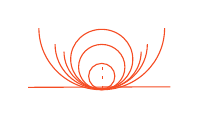
\begin{tikzpicture}[x=0.75pt,y=0.75pt,yscale=-1,xscale=1]
%uncomment if require: \path (0,330); %set diagram left start at 0, and has height of 330

%Shape: Arc [id:dp3367373231201912] 
\draw  [draw opacity=0] (307.2,172.86) .. controls (307.2,172.86) and (307.2,172.86) .. (307.2,172.86) .. controls (307.2,189.23) and (293.64,202.49) .. (276.92,202.49) .. controls (260.19,202.49) and (246.63,189.23) .. (246.63,172.86) .. controls (246.63,172.86) and (246.63,172.86) .. (246.63,172.86) -- (276.92,172.86) -- cycle ; \draw  [color={rgb, 255:red, 245; green, 76; blue, 35 }  ,draw opacity=1 ] (307.2,172.86) .. controls (307.2,172.86) and (307.2,172.86) .. (307.2,172.86) .. controls (307.2,189.23) and (293.64,202.49) .. (276.92,202.49) .. controls (260.19,202.49) and (246.63,189.23) .. (246.63,172.86) .. controls (246.63,172.86) and (246.63,172.86) .. (246.63,172.86) ;  
%Shape: Arc [id:dp7655049685942874] 
\draw  [draw opacity=0] (298.89,180.54) .. controls (298.89,192.48) and (288.94,202.15) .. (276.66,202.15) .. controls (264.37,202.15) and (254.42,192.48) .. (254.42,180.54) -- (276.66,180.54) -- cycle ; \draw  [color={rgb, 255:red, 245; green, 76; blue, 35 }  ,draw opacity=1 ] (298.89,180.54) .. controls (298.89,192.48) and (288.94,202.15) .. (276.66,202.15) .. controls (264.37,202.15) and (254.42,192.48) .. (254.42,180.54) ;  
%Shape: Arc [id:dp9171098404219228] 
\draw  [draw opacity=0] (295.91,184.11) .. controls (295.91,184.11) and (295.91,184.11) .. (295.91,184.11) .. controls (295.91,184.11) and (295.91,184.11) .. (295.91,184.11) .. controls (295.91,194.15) and (287.58,202.29) .. (277.32,202.29) .. controls (267.05,202.29) and (258.73,194.15) .. (258.73,184.11) -- (277.32,184.11) -- cycle ; \draw  [color={rgb, 255:red, 245; green, 76; blue, 35 }  ,draw opacity=1 ] (295.91,184.11) .. controls (295.91,184.11) and (295.91,184.11) .. (295.91,184.11) .. controls (295.91,184.11) and (295.91,184.11) .. (295.91,184.11) .. controls (295.91,194.15) and (287.58,202.29) .. (277.32,202.29) .. controls (267.05,202.29) and (258.73,194.15) .. (258.73,184.11) ;  
%Shape: Ellipse [id:dp7754727136568322] 
\draw  [color={rgb, 255:red, 245; green, 76; blue, 35 }  ,draw opacity=1 ] (265.75,191.57) .. controls (265.75,185.54) and (270.75,180.65) .. (276.92,180.65) .. controls (283.08,180.65) and (288.08,185.54) .. (288.08,191.57) .. controls (288.08,197.6) and (283.08,202.49) .. (276.92,202.49) .. controls (270.75,202.49) and (265.75,197.6) .. (265.75,191.57) -- cycle ;
%Shape: Ellipse [id:dp42805013541561066] 
\draw  [color={rgb, 255:red, 245; green, 76; blue, 35 }  ,draw opacity=1 ] (270.6,195.97) .. controls (270.6,192.56) and (273.43,189.79) .. (276.92,189.79) .. controls (280.4,189.79) and (283.23,192.56) .. (283.23,195.97) .. controls (283.23,199.39) and (280.4,202.15) .. (276.92,202.15) .. controls (273.43,202.15) and (270.6,199.39) .. (270.6,195.97) -- cycle ;
%Straight Lines [id:da8782637737908917] 
\draw [color={rgb, 255:red, 245; green, 76; blue, 35 }  ,draw opacity=1 ] [dash pattern={on 0.84pt off 2.51pt}]  (277.24,191.64) -- (277.24,202.56) ;
%Shape: Ellipse [id:dp2954580279871649] 
\draw  [color={rgb, 255:red, 245; green, 76; blue, 35 }  ,draw opacity=1 ] (261.95,187.77) .. controls (261.95,179.83) and (268.65,173.39) .. (276.92,173.39) .. controls (285.18,173.39) and (291.88,179.83) .. (291.88,187.77) .. controls (291.88,195.71) and (285.18,202.15) .. (276.92,202.15) .. controls (268.65,202.15) and (261.95,195.71) .. (261.95,187.77) -- cycle ;
%Straight Lines [id:da7332475670276889] 
\draw [color={rgb, 255:red, 245; green, 76; blue, 35 }  ,draw opacity=1 ]   (241.5,201.33) -- (310,201.08) ;




\end{tikzpicture}

\end{center}
Which looks like the wedge product of $n+1$ line segment with infinitely many circles. 
\end{frame}

\begin{frame}{$\phi\circ \psi$ is not a cover}
    The preimage of $U$ under this map looks like the following:
    \begin{center}
        

\tikzset{every picture/.style={line width=0.75pt}} %set default line width to 0.75pt        

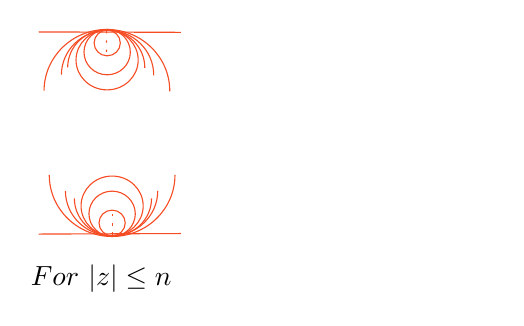
\begin{tikzpicture}[x=0.75pt,y=0.75pt,yscale=-1,xscale=1]
%uncomment if require: \path (0,330); %set diagram left start at 0, and has height of 330

%Shape: Arc [id:dp3367373231201912] 
\draw  [draw opacity=0] (305.7,170.3) .. controls (305.7,170.3) and (305.7,170.3) .. (305.7,170.3) .. controls (305.7,186.66) and (292.14,199.93) .. (275.42,199.93) .. controls (258.69,199.93) and (245.13,186.66) .. (245.13,170.3) .. controls (245.13,170.3) and (245.13,170.3) .. (245.13,170.3) -- (275.42,170.3) -- cycle ; \draw  [color={rgb, 255:red, 245; green, 76; blue, 35 }  ,draw opacity=1 ] (305.7,170.3) .. controls (305.7,170.3) and (305.7,170.3) .. (305.7,170.3) .. controls (305.7,186.66) and (292.14,199.93) .. (275.42,199.93) .. controls (258.69,199.93) and (245.13,186.66) .. (245.13,170.3) .. controls (245.13,170.3) and (245.13,170.3) .. (245.13,170.3) ;  
%Shape: Arc [id:dp7655049685942874] 
\draw  [draw opacity=0] (297.39,177.98) .. controls (297.39,189.91) and (287.44,199.59) .. (275.16,199.59) .. controls (262.87,199.59) and (252.92,189.91) .. (252.92,177.98) -- (275.16,177.98) -- cycle ; \draw  [color={rgb, 255:red, 245; green, 76; blue, 35 }  ,draw opacity=1 ] (297.39,177.98) .. controls (297.39,189.91) and (287.44,199.59) .. (275.16,199.59) .. controls (262.87,199.59) and (252.92,189.91) .. (252.92,177.98) ;  
%Shape: Arc [id:dp9171098404219228] 
\draw  [draw opacity=0] (294.41,181.55) .. controls (294.41,181.55) and (294.41,181.55) .. (294.41,181.55) .. controls (294.41,181.55) and (294.41,181.55) .. (294.41,181.55) .. controls (294.41,191.59) and (286.08,199.73) .. (275.82,199.73) .. controls (265.55,199.73) and (257.23,191.59) .. (257.23,181.55) -- (275.82,181.55) -- cycle ; \draw  [color={rgb, 255:red, 245; green, 76; blue, 35 }  ,draw opacity=1 ] (294.41,181.55) .. controls (294.41,181.55) and (294.41,181.55) .. (294.41,181.55) .. controls (294.41,181.55) and (294.41,181.55) .. (294.41,181.55) .. controls (294.41,191.59) and (286.08,199.73) .. (275.82,199.73) .. controls (265.55,199.73) and (257.23,191.59) .. (257.23,181.55) ;  
%Shape: Ellipse [id:dp7754727136568322] 
\draw  [color={rgb, 255:red, 245; green, 76; blue, 35 }  ,draw opacity=1 ] (264.25,189.01) .. controls (264.25,182.98) and (269.25,178.09) .. (275.42,178.09) .. controls (281.58,178.09) and (286.58,182.98) .. (286.58,189.01) .. controls (286.58,195.04) and (281.58,199.93) .. (275.42,199.93) .. controls (269.25,199.93) and (264.25,195.04) .. (264.25,189.01) -- cycle ;
%Shape: Ellipse [id:dp42805013541561066] 
\draw  [color={rgb, 255:red, 245; green, 76; blue, 35 }  ,draw opacity=1 ] (269.1,193.41) .. controls (269.1,190) and (271.93,187.23) .. (275.42,187.23) .. controls (278.9,187.23) and (281.73,190) .. (281.73,193.41) .. controls (281.73,196.82) and (278.9,199.59) .. (275.42,199.59) .. controls (271.93,199.59) and (269.1,196.82) .. (269.1,193.41) -- cycle ;
%Straight Lines [id:da8782637737908917] 
\draw [color={rgb, 255:red, 245; green, 76; blue, 35 }  ,draw opacity=1 ] [dash pattern={on 0.84pt off 2.51pt}]  (275.74,189.08) -- (275.74,200) ;
%Shape: Ellipse [id:dp2954580279871649] 
\draw  [color={rgb, 255:red, 245; green, 76; blue, 35 }  ,draw opacity=1 ] (260.45,185.21) .. controls (260.45,177.26) and (267.15,170.82) .. (275.42,170.82) .. controls (283.68,170.82) and (290.38,177.26) .. (290.38,185.21) .. controls (290.38,193.15) and (283.68,199.59) .. (275.42,199.59) .. controls (267.15,199.59) and (260.45,193.15) .. (260.45,185.21) -- cycle ;
%Straight Lines [id:da7332475670276889] 
\draw [color={rgb, 255:red, 245; green, 76; blue, 35 }  ,draw opacity=1 ]   (240,198.77) -- (308.5,198.52) ;
%Shape: Arc [id:dp8866692252729794] 
\draw  [draw opacity=0] (242.62,129.63) .. controls (242.62,129.63) and (242.62,129.63) .. (242.62,129.63) .. controls (242.73,113.26) and (256.37,100.09) .. (273.09,100.19) .. controls (289.82,100.3) and (303.29,113.65) .. (303.19,130.01) .. controls (303.19,130.01) and (303.19,130.01) .. (303.19,130.01) -- (272.91,129.82) -- cycle ; \draw  [color={rgb, 255:red, 245; green, 76; blue, 35 }  ,draw opacity=1 ] (242.62,129.63) .. controls (242.62,129.63) and (242.62,129.63) .. (242.62,129.63) .. controls (242.73,113.26) and (256.37,100.09) .. (273.09,100.19) .. controls (289.82,100.3) and (303.29,113.65) .. (303.19,130.01) .. controls (303.19,130.01) and (303.19,130.01) .. (303.19,130.01) ;  
%Shape: Arc [id:dp8993370067461369] 
\draw  [draw opacity=0] (250.98,122) .. controls (251.05,110.07) and (261.07,100.45) .. (273.35,100.53) .. controls (285.63,100.61) and (295.53,110.35) .. (295.45,122.28) -- (273.21,122.14) -- cycle ; \draw  [color={rgb, 255:red, 245; green, 76; blue, 35 }  ,draw opacity=1 ] (250.98,122) .. controls (251.05,110.07) and (261.07,100.45) .. (273.35,100.53) .. controls (285.63,100.61) and (295.53,110.35) .. (295.45,122.28) ;  
%Shape: Arc [id:dp5917617333796023] 
\draw  [draw opacity=0] (253.99,118.45) .. controls (253.99,118.45) and (253.99,118.45) .. (253.99,118.45) .. controls (253.99,118.45) and (253.99,118.45) .. (253.99,118.45) .. controls (254.05,108.41) and (262.42,100.32) .. (272.69,100.39) .. controls (282.95,100.45) and (291.22,108.64) .. (291.16,118.69) -- (272.57,118.57) -- cycle ; \draw  [color={rgb, 255:red, 245; green, 76; blue, 35 }  ,draw opacity=1 ] (253.99,118.45) .. controls (253.99,118.45) and (253.99,118.45) .. (253.99,118.45) .. controls (253.99,118.45) and (253.99,118.45) .. (253.99,118.45) .. controls (254.05,108.41) and (262.42,100.32) .. (272.69,100.39) .. controls (282.95,100.45) and (291.22,108.64) .. (291.16,118.69) ;  
%Shape: Ellipse [id:dp33142315050842575] 
\draw  [color={rgb, 255:red, 245; green, 76; blue, 35 }  ,draw opacity=1 ] (284.19,111.18) .. controls (284.15,117.21) and (279.12,122.07) .. (272.96,122.03) .. controls (266.79,121.99) and (261.82,117.07) .. (261.86,111.04) .. controls (261.9,105.01) and (266.93,100.15) .. (273.09,100.19) .. controls (279.26,100.23) and (284.22,105.15) .. (284.19,111.18) -- cycle ;
%Shape: Ellipse [id:dp8950325891645826] 
\draw  [color={rgb, 255:red, 245; green, 76; blue, 35 }  ,draw opacity=1 ] (279.37,106.75) .. controls (279.35,110.16) and (276.5,112.91) .. (273.01,112.89) .. controls (269.52,112.87) and (266.71,110.08) .. (266.74,106.67) .. controls (266.76,103.26) and (269.6,100.51) .. (273.09,100.53) .. controls (276.58,100.55) and (279.39,103.34) .. (279.37,106.75) -- cycle ;
%Straight Lines [id:da4554817296987891] 
\draw [color={rgb, 255:red, 245; green, 76; blue, 35 }  ,draw opacity=1 ] [dash pattern={on 0.84pt off 2.51pt}]  (272.7,111.04) -- (272.77,100.12) ;
%Shape: Ellipse [id:dp1567169696587729] 
\draw  [color={rgb, 255:red, 245; green, 76; blue, 35 }  ,draw opacity=1 ] (287.97,115.01) .. controls (287.92,122.95) and (281.18,129.35) .. (272.91,129.3) .. controls (264.64,129.24) and (257.98,122.76) .. (258.03,114.82) .. controls (258.08,106.87) and (264.82,100.48) .. (273.09,100.53) .. controls (281.36,100.58) and (288.02,107.06) .. (287.97,115.01) -- cycle ;
%Straight Lines [id:da01360265720570153] 
\draw [color={rgb, 255:red, 245; green, 76; blue, 35 }  ,draw opacity=1 ]   (308.5,101.57) -- (240,101.39) ;
%Shape: Arc [id:dp42777306144239347] 
\draw  [draw opacity=0] (453.41,168.87) .. controls (453.41,168.87) and (453.41,168.87) .. (453.41,168.87) .. controls (453.41,185.24) and (439.86,198.5) .. (423.13,198.5) .. controls (406.4,198.5) and (392.84,185.24) .. (392.84,168.87) .. controls (392.84,168.87) and (392.84,168.87) .. (392.84,168.87) -- (423.13,168.87) -- cycle ; \draw  [color={rgb, 255:red, 245; green, 76; blue, 35 }  ,draw opacity=1 ] (453.41,168.87) .. controls (453.41,168.87) and (453.41,168.87) .. (453.41,168.87) .. controls (453.41,185.24) and (439.86,198.5) .. (423.13,198.5) .. controls (406.4,198.5) and (392.84,185.24) .. (392.84,168.87) .. controls (392.84,168.87) and (392.84,168.87) .. (392.84,168.87) ;  
%Shape: Arc [id:dp797304877230008] 
\draw  [draw opacity=0] (445.11,176.55) .. controls (445.11,188.48) and (435.15,198.16) .. (422.87,198.16) .. controls (410.59,198.16) and (400.63,188.48) .. (400.63,176.55) -- (422.87,176.55) -- cycle ; \draw  [color={rgb, 255:red, 245; green, 76; blue, 35 }  ,draw opacity=1 ] (445.11,176.55) .. controls (445.11,188.48) and (435.15,198.16) .. (422.87,198.16) .. controls (410.59,198.16) and (400.63,188.48) .. (400.63,176.55) ;  
%Shape: Arc [id:dp8908957957332029] 
\draw  [draw opacity=0] (442.12,180.12) .. controls (442.12,180.12) and (442.12,180.12) .. (442.12,180.12) .. controls (442.12,180.12) and (442.12,180.12) .. (442.12,180.12) .. controls (442.12,190.16) and (433.8,198.3) .. (423.53,198.3) .. controls (413.27,198.3) and (404.95,190.16) .. (404.95,180.12) -- (423.53,180.12) -- cycle ; \draw  [color={rgb, 255:red, 245; green, 76; blue, 35 }  ,draw opacity=1 ] (442.12,180.12) .. controls (442.12,180.12) and (442.12,180.12) .. (442.12,180.12) .. controls (442.12,180.12) and (442.12,180.12) .. (442.12,180.12) .. controls (442.12,190.16) and (433.8,198.3) .. (423.53,198.3) .. controls (413.27,198.3) and (404.95,190.16) .. (404.95,180.12) ;  
%Shape: Ellipse [id:dp03680214293557027] 
\draw  [color={rgb, 255:red, 245; green, 76; blue, 35 }  ,draw opacity=1 ] (411.97,187.58) .. controls (411.97,181.55) and (416.96,176.66) .. (423.13,176.66) .. controls (429.29,176.66) and (434.29,181.55) .. (434.29,187.58) .. controls (434.29,193.61) and (429.29,198.5) .. (423.13,198.5) .. controls (416.96,198.5) and (411.97,193.61) .. (411.97,187.58) -- cycle ;
%Shape: Ellipse [id:dp48314716650274747] 
\draw  [color={rgb, 255:red, 245; green, 76; blue, 35 }  ,draw opacity=1 ] (416.81,191.98) .. controls (416.81,188.57) and (419.64,185.8) .. (423.13,185.8) .. controls (426.62,185.8) and (429.45,188.57) .. (429.45,191.98) .. controls (429.45,195.4) and (426.62,198.16) .. (423.13,198.16) .. controls (419.64,198.16) and (416.81,195.4) .. (416.81,191.98) -- cycle ;
%Straight Lines [id:da6993970124426362] 
\draw [color={rgb, 255:red, 245; green, 76; blue, 35 }  ,draw opacity=1 ] [dash pattern={on 0.84pt off 2.51pt}]  (423.46,187.65) -- (423.46,198.57) ;
%Shape: Ellipse [id:dp025809737358414853] 
\draw  [color={rgb, 255:red, 245; green, 76; blue, 35 }  ,draw opacity=1 ] (408.16,183.78) .. controls (408.16,175.83) and (414.86,169.39) .. (423.13,169.39) .. controls (431.4,169.39) and (438.1,175.83) .. (438.1,183.78) .. controls (438.1,191.72) and (431.4,198.16) .. (423.13,198.16) .. controls (414.86,198.16) and (408.16,191.72) .. (408.16,183.78) -- cycle ;
%Straight Lines [id:da6887063203021668] 
\draw [color={rgb, 255:red, 245; green, 76; blue, 35 }  ,draw opacity=1 ]   (387.71,197.34) -- (456.21,197.09) ;
%Shape: Arc [id:dp3693665851394208] 
\draw  [draw opacity=0] (392.62,129.63) .. controls (392.62,129.63) and (392.62,129.63) .. (392.62,129.63) .. controls (392.73,113.26) and (406.37,100.09) .. (423.09,100.19) .. controls (439.82,100.3) and (453.29,113.65) .. (453.19,130.01) .. controls (453.19,130.01) and (453.19,130.01) .. (453.19,130.01) -- (422.91,129.82) -- cycle ; \draw  [color={rgb, 255:red, 245; green, 76; blue, 35 }  ,draw opacity=1 ] (392.62,129.63) .. controls (392.62,129.63) and (392.62,129.63) .. (392.62,129.63) .. controls (392.73,113.26) and (406.37,100.09) .. (423.09,100.19) .. controls (439.82,100.3) and (453.29,113.65) .. (453.19,130.01) .. controls (453.19,130.01) and (453.19,130.01) .. (453.19,130.01) ;  
%Shape: Arc [id:dp8338437028438305] 
\draw  [draw opacity=0] (400.98,122) .. controls (401.05,110.07) and (411.07,100.45) .. (423.35,100.53) .. controls (435.63,100.61) and (445.53,110.35) .. (445.45,122.28) -- (423.21,122.14) -- cycle ; \draw  [color={rgb, 255:red, 245; green, 76; blue, 35 }  ,draw opacity=1 ] (400.98,122) .. controls (401.05,110.07) and (411.07,100.45) .. (423.35,100.53) .. controls (435.63,100.61) and (445.53,110.35) .. (445.45,122.28) ;  
%Shape: Arc [id:dp8090516680248827] 
\draw  [draw opacity=0] (403.99,118.45) .. controls (403.99,118.45) and (403.99,118.45) .. (403.99,118.45) .. controls (403.99,118.45) and (403.99,118.45) .. (403.99,118.45) .. controls (404.05,108.41) and (412.42,100.32) .. (422.69,100.39) .. controls (432.95,100.45) and (441.22,108.64) .. (441.16,118.69) -- (422.57,118.57) -- cycle ; \draw  [color={rgb, 255:red, 245; green, 76; blue, 35 }  ,draw opacity=1 ] (403.99,118.45) .. controls (403.99,118.45) and (403.99,118.45) .. (403.99,118.45) .. controls (403.99,118.45) and (403.99,118.45) .. (403.99,118.45) .. controls (404.05,108.41) and (412.42,100.32) .. (422.69,100.39) .. controls (432.95,100.45) and (441.22,108.64) .. (441.16,118.69) ;  
%Shape: Ellipse [id:dp8978682080533286] 
\draw  [color={rgb, 255:red, 245; green, 76; blue, 35 }  ,draw opacity=1 ] (434.19,111.18) .. controls (434.15,117.21) and (429.12,122.07) .. (422.96,122.03) .. controls (416.79,121.99) and (411.82,117.07) .. (411.86,111.04) .. controls (411.9,105.01) and (416.93,100.15) .. (423.09,100.19) .. controls (429.26,100.23) and (434.22,105.15) .. (434.19,111.18) -- cycle ;
%Shape: Ellipse [id:dp22773855421731792] 
\draw  [color={rgb, 255:red, 245; green, 76; blue, 35 }  ,draw opacity=1 ] (429.37,106.75) .. controls (429.35,110.16) and (426.5,112.91) .. (423.01,112.89) .. controls (419.52,112.87) and (416.71,110.08) .. (416.74,106.67) .. controls (416.76,103.26) and (419.6,100.51) .. (423.09,100.53) .. controls (426.58,100.55) and (429.39,103.34) .. (429.37,106.75) -- cycle ;
%Straight Lines [id:da891993741817402] 
\draw [color={rgb, 255:red, 245; green, 76; blue, 35 }  ,draw opacity=1 ] [dash pattern={on 0.84pt off 2.51pt}]  (422.7,111.04) -- (422.77,100.12) ;
%Shape: Ellipse [id:dp37710316486801587] 
\draw  [color={rgb, 255:red, 245; green, 76; blue, 35 }  ,draw opacity=1 ] (437.97,115.01) .. controls (437.92,122.95) and (431.18,129.35) .. (422.91,129.3) .. controls (414.64,129.24) and (407.98,122.76) .. (408.03,114.82) .. controls (408.08,106.87) and (414.82,100.48) .. (423.09,100.53) .. controls (431.36,100.58) and (438.02,107.06) .. (437.97,115.01) -- cycle ;
%Straight Lines [id:da13911890461318233] 
\draw [color={rgb, 255:red, 245; green, 76; blue, 35 }  ,draw opacity=1 ]   (458.5,101.57) -- (390,101.39) ;
%Straight Lines [id:da14513158759358802] 
\draw [color={rgb, 255:red, 245; green, 76; blue, 35 }  ,draw opacity=1 ]   (403.99,118.45) -- (404.95,180.12) ;
%Straight Lines [id:da8217624934121862] 
\draw [color={rgb, 255:red, 245; green, 76; blue, 35 }  ,draw opacity=1 ]   (441.16,118.45) -- (442.12,180.12) ;
%Flowchart: Process [id:dp12758515513568502] 
\draw  [draw opacity=0][fill={rgb, 255:red, 255; green, 255; blue, 255 }  ,fill opacity=1 ] (379.81,99.6) -- (460.14,99.6) -- (460.14,229.33) -- (379.81,229.33) -- cycle ;

% Text Node
\draw (235,212.4) node [anchor=north west][inner sep=0.75pt]    {$For\ |z|\leq n$};


\end{tikzpicture}

    \end{center}
\end{frame}

\begin{frame}{$\phi\circ \psi$ is not a cover}
    The preimage of $U$ under this map looks like the following:
    \begin{center}
        

\tikzset{every picture/.style={line width=0.75pt}} %set default line width to 0.75pt        

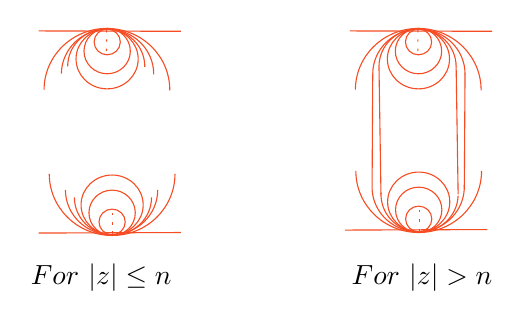
\begin{tikzpicture}[x=0.75pt,y=0.75pt,yscale=-1,xscale=1]
%uncomment if require: \path (0,330); %set diagram left start at 0, and has height of 330

%Shape: Arc [id:dp3367373231201912] 
\draw  [draw opacity=0] (305.7,170.3) .. controls (305.7,170.3) and (305.7,170.3) .. (305.7,170.3) .. controls (305.7,186.66) and (292.14,199.93) .. (275.42,199.93) .. controls (258.69,199.93) and (245.13,186.66) .. (245.13,170.3) .. controls (245.13,170.3) and (245.13,170.3) .. (245.13,170.3) -- (275.42,170.3) -- cycle ; \draw  [color={rgb, 255:red, 245; green, 76; blue, 35 }  ,draw opacity=1 ] (305.7,170.3) .. controls (305.7,170.3) and (305.7,170.3) .. (305.7,170.3) .. controls (305.7,186.66) and (292.14,199.93) .. (275.42,199.93) .. controls (258.69,199.93) and (245.13,186.66) .. (245.13,170.3) .. controls (245.13,170.3) and (245.13,170.3) .. (245.13,170.3) ;  
%Shape: Arc [id:dp7655049685942874] 
\draw  [draw opacity=0] (297.39,177.98) .. controls (297.39,189.91) and (287.44,199.59) .. (275.16,199.59) .. controls (262.87,199.59) and (252.92,189.91) .. (252.92,177.98) -- (275.16,177.98) -- cycle ; \draw  [color={rgb, 255:red, 245; green, 76; blue, 35 }  ,draw opacity=1 ] (297.39,177.98) .. controls (297.39,189.91) and (287.44,199.59) .. (275.16,199.59) .. controls (262.87,199.59) and (252.92,189.91) .. (252.92,177.98) ;  
%Shape: Arc [id:dp9171098404219228] 
\draw  [draw opacity=0] (294.41,181.55) .. controls (294.41,181.55) and (294.41,181.55) .. (294.41,181.55) .. controls (294.41,181.55) and (294.41,181.55) .. (294.41,181.55) .. controls (294.41,191.59) and (286.08,199.73) .. (275.82,199.73) .. controls (265.55,199.73) and (257.23,191.59) .. (257.23,181.55) -- (275.82,181.55) -- cycle ; \draw  [color={rgb, 255:red, 245; green, 76; blue, 35 }  ,draw opacity=1 ] (294.41,181.55) .. controls (294.41,181.55) and (294.41,181.55) .. (294.41,181.55) .. controls (294.41,181.55) and (294.41,181.55) .. (294.41,181.55) .. controls (294.41,191.59) and (286.08,199.73) .. (275.82,199.73) .. controls (265.55,199.73) and (257.23,191.59) .. (257.23,181.55) ;  
%Shape: Ellipse [id:dp7754727136568322] 
\draw  [color={rgb, 255:red, 245; green, 76; blue, 35 }  ,draw opacity=1 ] (264.25,189.01) .. controls (264.25,182.98) and (269.25,178.09) .. (275.42,178.09) .. controls (281.58,178.09) and (286.58,182.98) .. (286.58,189.01) .. controls (286.58,195.04) and (281.58,199.93) .. (275.42,199.93) .. controls (269.25,199.93) and (264.25,195.04) .. (264.25,189.01) -- cycle ;
%Shape: Ellipse [id:dp42805013541561066] 
\draw  [color={rgb, 255:red, 245; green, 76; blue, 35 }  ,draw opacity=1 ] (269.1,193.41) .. controls (269.1,190) and (271.93,187.23) .. (275.42,187.23) .. controls (278.9,187.23) and (281.73,190) .. (281.73,193.41) .. controls (281.73,196.82) and (278.9,199.59) .. (275.42,199.59) .. controls (271.93,199.59) and (269.1,196.82) .. (269.1,193.41) -- cycle ;
%Straight Lines [id:da8782637737908917] 
\draw [color={rgb, 255:red, 245; green, 76; blue, 35 }  ,draw opacity=1 ] [dash pattern={on 0.84pt off 2.51pt}]  (275.74,189.08) -- (275.74,200) ;
%Shape: Ellipse [id:dp2954580279871649] 
\draw  [color={rgb, 255:red, 245; green, 76; blue, 35 }  ,draw opacity=1 ] (260.45,185.21) .. controls (260.45,177.26) and (267.15,170.82) .. (275.42,170.82) .. controls (283.68,170.82) and (290.38,177.26) .. (290.38,185.21) .. controls (290.38,193.15) and (283.68,199.59) .. (275.42,199.59) .. controls (267.15,199.59) and (260.45,193.15) .. (260.45,185.21) -- cycle ;
%Straight Lines [id:da7332475670276889] 
\draw [color={rgb, 255:red, 245; green, 76; blue, 35 }  ,draw opacity=1 ]   (240,198.77) -- (308.5,198.52) ;
%Shape: Arc [id:dp8866692252729794] 
\draw  [draw opacity=0] (242.62,129.63) .. controls (242.62,129.63) and (242.62,129.63) .. (242.62,129.63) .. controls (242.73,113.26) and (256.37,100.09) .. (273.09,100.19) .. controls (289.82,100.3) and (303.29,113.65) .. (303.19,130.01) .. controls (303.19,130.01) and (303.19,130.01) .. (303.19,130.01) -- (272.91,129.82) -- cycle ; \draw  [color={rgb, 255:red, 245; green, 76; blue, 35 }  ,draw opacity=1 ] (242.62,129.63) .. controls (242.62,129.63) and (242.62,129.63) .. (242.62,129.63) .. controls (242.73,113.26) and (256.37,100.09) .. (273.09,100.19) .. controls (289.82,100.3) and (303.29,113.65) .. (303.19,130.01) .. controls (303.19,130.01) and (303.19,130.01) .. (303.19,130.01) ;  
%Shape: Arc [id:dp8993370067461369] 
\draw  [draw opacity=0] (250.98,122) .. controls (251.05,110.07) and (261.07,100.45) .. (273.35,100.53) .. controls (285.63,100.61) and (295.53,110.35) .. (295.45,122.28) -- (273.21,122.14) -- cycle ; \draw  [color={rgb, 255:red, 245; green, 76; blue, 35 }  ,draw opacity=1 ] (250.98,122) .. controls (251.05,110.07) and (261.07,100.45) .. (273.35,100.53) .. controls (285.63,100.61) and (295.53,110.35) .. (295.45,122.28) ;  
%Shape: Arc [id:dp5917617333796023] 
\draw  [draw opacity=0] (253.99,118.45) .. controls (253.99,118.45) and (253.99,118.45) .. (253.99,118.45) .. controls (253.99,118.45) and (253.99,118.45) .. (253.99,118.45) .. controls (254.05,108.41) and (262.42,100.32) .. (272.69,100.39) .. controls (282.95,100.45) and (291.22,108.64) .. (291.16,118.69) -- (272.57,118.57) -- cycle ; \draw  [color={rgb, 255:red, 245; green, 76; blue, 35 }  ,draw opacity=1 ] (253.99,118.45) .. controls (253.99,118.45) and (253.99,118.45) .. (253.99,118.45) .. controls (253.99,118.45) and (253.99,118.45) .. (253.99,118.45) .. controls (254.05,108.41) and (262.42,100.32) .. (272.69,100.39) .. controls (282.95,100.45) and (291.22,108.64) .. (291.16,118.69) ;  
%Shape: Ellipse [id:dp33142315050842575] 
\draw  [color={rgb, 255:red, 245; green, 76; blue, 35 }  ,draw opacity=1 ] (284.19,111.18) .. controls (284.15,117.21) and (279.12,122.07) .. (272.96,122.03) .. controls (266.79,121.99) and (261.82,117.07) .. (261.86,111.04) .. controls (261.9,105.01) and (266.93,100.15) .. (273.09,100.19) .. controls (279.26,100.23) and (284.22,105.15) .. (284.19,111.18) -- cycle ;
%Shape: Ellipse [id:dp8950325891645826] 
\draw  [color={rgb, 255:red, 245; green, 76; blue, 35 }  ,draw opacity=1 ] (279.37,106.75) .. controls (279.35,110.16) and (276.5,112.91) .. (273.01,112.89) .. controls (269.52,112.87) and (266.71,110.08) .. (266.74,106.67) .. controls (266.76,103.26) and (269.6,100.51) .. (273.09,100.53) .. controls (276.58,100.55) and (279.39,103.34) .. (279.37,106.75) -- cycle ;
%Straight Lines [id:da4554817296987891] 
\draw [color={rgb, 255:red, 245; green, 76; blue, 35 }  ,draw opacity=1 ] [dash pattern={on 0.84pt off 2.51pt}]  (272.7,111.04) -- (272.77,100.12) ;
%Shape: Ellipse [id:dp1567169696587729] 
\draw  [color={rgb, 255:red, 245; green, 76; blue, 35 }  ,draw opacity=1 ] (287.97,115.01) .. controls (287.92,122.95) and (281.18,129.35) .. (272.91,129.3) .. controls (264.64,129.24) and (257.98,122.76) .. (258.03,114.82) .. controls (258.08,106.87) and (264.82,100.48) .. (273.09,100.53) .. controls (281.36,100.58) and (288.02,107.06) .. (287.97,115.01) -- cycle ;
%Straight Lines [id:da01360265720570153] 
\draw [color={rgb, 255:red, 245; green, 76; blue, 35 }  ,draw opacity=1 ]   (308.5,101.57) -- (240,101.39) ;
%Shape: Arc [id:dp42777306144239347] 
\draw  [draw opacity=0] (453.41,168.87) .. controls (453.41,168.87) and (453.41,168.87) .. (453.41,168.87) .. controls (453.41,185.24) and (439.86,198.5) .. (423.13,198.5) .. controls (406.4,198.5) and (392.84,185.24) .. (392.84,168.87) .. controls (392.84,168.87) and (392.84,168.87) .. (392.84,168.87) -- (423.13,168.87) -- cycle ; \draw  [color={rgb, 255:red, 245; green, 76; blue, 35 }  ,draw opacity=1 ] (453.41,168.87) .. controls (453.41,168.87) and (453.41,168.87) .. (453.41,168.87) .. controls (453.41,185.24) and (439.86,198.5) .. (423.13,198.5) .. controls (406.4,198.5) and (392.84,185.24) .. (392.84,168.87) .. controls (392.84,168.87) and (392.84,168.87) .. (392.84,168.87) ;  
%Shape: Arc [id:dp797304877230008] 
\draw  [draw opacity=0] (445.08,175.43) .. controls (445.68,187.35) and (436.22,197.52) .. (423.96,198.13) .. controls (411.69,198.75) and (401.26,189.59) .. (400.66,177.66) -- (422.87,176.55) -- cycle ; \draw  [color={rgb, 255:red, 245; green, 76; blue, 35 }  ,draw opacity=1 ] (445.08,175.43) .. controls (445.68,187.35) and (436.22,197.52) .. (423.96,198.13) .. controls (411.69,198.75) and (401.26,189.59) .. (400.66,177.66) ;  
%Shape: Arc [id:dp8908957957332029] 
\draw  [draw opacity=0] (442.11,180.77) .. controls (442.11,180.77) and (442.11,180.77) .. (442.11,180.77) .. controls (442.11,180.77) and (442.11,180.77) .. (442.11,180.77) .. controls (441.76,190.81) and (433.15,198.65) .. (422.89,198.29) .. controls (412.63,197.93) and (404.6,189.5) .. (404.96,179.46) -- (423.53,180.12) -- cycle ; \draw  [color={rgb, 255:red, 245; green, 76; blue, 35 }  ,draw opacity=1 ] (442.11,180.77) .. controls (442.11,180.77) and (442.11,180.77) .. (442.11,180.77) .. controls (442.11,180.77) and (442.11,180.77) .. (442.11,180.77) .. controls (441.76,190.81) and (433.15,198.65) .. (422.89,198.29) .. controls (412.63,197.93) and (404.6,189.5) .. (404.96,179.46) ;  
%Shape: Ellipse [id:dp03680214293557027] 
\draw  [color={rgb, 255:red, 245; green, 76; blue, 35 }  ,draw opacity=1 ] (411.97,187.58) .. controls (411.97,181.55) and (416.96,176.66) .. (423.13,176.66) .. controls (429.29,176.66) and (434.29,181.55) .. (434.29,187.58) .. controls (434.29,193.61) and (429.29,198.5) .. (423.13,198.5) .. controls (416.96,198.5) and (411.97,193.61) .. (411.97,187.58) -- cycle ;
%Shape: Ellipse [id:dp48314716650274747] 
\draw  [color={rgb, 255:red, 245; green, 76; blue, 35 }  ,draw opacity=1 ] (416.81,191.98) .. controls (416.81,188.57) and (419.64,185.8) .. (423.13,185.8) .. controls (426.62,185.8) and (429.45,188.57) .. (429.45,191.98) .. controls (429.45,195.4) and (426.62,198.16) .. (423.13,198.16) .. controls (419.64,198.16) and (416.81,195.4) .. (416.81,191.98) -- cycle ;
%Straight Lines [id:da6993970124426362] 
\draw [color={rgb, 255:red, 245; green, 76; blue, 35 }  ,draw opacity=1 ] [dash pattern={on 0.84pt off 2.51pt}]  (423.46,187.65) -- (423.46,198.57) ;
%Shape: Ellipse [id:dp025809737358414853] 
\draw  [color={rgb, 255:red, 245; green, 76; blue, 35 }  ,draw opacity=1 ] (408.16,183.78) .. controls (408.16,175.83) and (414.86,169.39) .. (423.13,169.39) .. controls (431.4,169.39) and (438.1,175.83) .. (438.1,183.78) .. controls (438.1,191.72) and (431.4,198.16) .. (423.13,198.16) .. controls (414.86,198.16) and (408.16,191.72) .. (408.16,183.78) -- cycle ;
%Straight Lines [id:da6887063203021668] 
\draw [color={rgb, 255:red, 245; green, 76; blue, 35 }  ,draw opacity=1 ]   (387.71,197.34) -- (456.21,197.09) ;
%Shape: Arc [id:dp3693665851394208] 
\draw  [draw opacity=0] (392.62,129.63) .. controls (392.62,129.63) and (392.62,129.63) .. (392.62,129.63) .. controls (392.73,113.26) and (406.37,100.09) .. (423.09,100.19) .. controls (439.82,100.3) and (453.29,113.65) .. (453.19,130.01) .. controls (453.19,130.01) and (453.19,130.01) .. (453.19,130.01) -- (422.91,129.82) -- cycle ; \draw  [color={rgb, 255:red, 245; green, 76; blue, 35 }  ,draw opacity=1 ] (392.62,129.63) .. controls (392.62,129.63) and (392.62,129.63) .. (392.62,129.63) .. controls (392.73,113.26) and (406.37,100.09) .. (423.09,100.19) .. controls (439.82,100.3) and (453.29,113.65) .. (453.19,130.01) .. controls (453.19,130.01) and (453.19,130.01) .. (453.19,130.01) ;  
%Shape: Arc [id:dp8338437028438305] 
\draw  [draw opacity=0] (400.98,122) .. controls (401.05,110.07) and (411.07,100.45) .. (423.35,100.53) .. controls (435.63,100.61) and (445.53,110.35) .. (445.45,122.28) -- (423.21,122.14) -- cycle ; \draw  [color={rgb, 255:red, 245; green, 76; blue, 35 }  ,draw opacity=1 ] (400.98,122) .. controls (401.05,110.07) and (411.07,100.45) .. (423.35,100.53) .. controls (435.63,100.61) and (445.53,110.35) .. (445.45,122.28) ;  
%Shape: Arc [id:dp8090516680248827] 
\draw  [draw opacity=0] (403.99,118.45) .. controls (403.99,118.45) and (403.99,118.45) .. (403.99,118.45) .. controls (403.99,118.45) and (403.99,118.45) .. (403.99,118.45) .. controls (404.05,108.41) and (412.42,100.32) .. (422.69,100.39) .. controls (432.95,100.45) and (441.22,108.64) .. (441.16,118.69) -- (422.57,118.57) -- cycle ; \draw  [color={rgb, 255:red, 245; green, 76; blue, 35 }  ,draw opacity=1 ] (403.99,118.45) .. controls (403.99,118.45) and (403.99,118.45) .. (403.99,118.45) .. controls (403.99,118.45) and (403.99,118.45) .. (403.99,118.45) .. controls (404.05,108.41) and (412.42,100.32) .. (422.69,100.39) .. controls (432.95,100.45) and (441.22,108.64) .. (441.16,118.69) ;  
%Shape: Ellipse [id:dp8978682080533286] 
\draw  [color={rgb, 255:red, 245; green, 76; blue, 35 }  ,draw opacity=1 ] (434.19,111.18) .. controls (434.15,117.21) and (429.12,122.07) .. (422.96,122.03) .. controls (416.79,121.99) and (411.82,117.07) .. (411.86,111.04) .. controls (411.9,105.01) and (416.93,100.15) .. (423.09,100.19) .. controls (429.26,100.23) and (434.22,105.15) .. (434.19,111.18) -- cycle ;
%Shape: Ellipse [id:dp22773855421731792] 
\draw  [color={rgb, 255:red, 245; green, 76; blue, 35 }  ,draw opacity=1 ] (429.37,106.75) .. controls (429.35,110.16) and (426.5,112.91) .. (423.01,112.89) .. controls (419.52,112.87) and (416.71,110.08) .. (416.74,106.67) .. controls (416.76,103.26) and (419.6,100.51) .. (423.09,100.53) .. controls (426.58,100.55) and (429.39,103.34) .. (429.37,106.75) -- cycle ;
%Straight Lines [id:da891993741817402] 
\draw [color={rgb, 255:red, 245; green, 76; blue, 35 }  ,draw opacity=1 ] [dash pattern={on 0.84pt off 2.51pt}]  (422.7,111.04) -- (422.77,100.12) ;
%Shape: Ellipse [id:dp37710316486801587] 
\draw  [color={rgb, 255:red, 245; green, 76; blue, 35 }  ,draw opacity=1 ] (437.97,115.01) .. controls (437.92,122.95) and (431.18,129.35) .. (422.91,129.3) .. controls (414.64,129.24) and (407.98,122.76) .. (408.03,114.82) .. controls (408.08,106.87) and (414.82,100.48) .. (423.09,100.53) .. controls (431.36,100.58) and (438.02,107.06) .. (437.97,115.01) -- cycle ;
%Straight Lines [id:da13911890461318233] 
\draw [color={rgb, 255:red, 245; green, 76; blue, 35 }  ,draw opacity=1 ]   (458.5,101.57) -- (390,101.39) ;
%Straight Lines [id:da14513158759358802] 
\draw [color={rgb, 255:red, 245; green, 76; blue, 35 }  ,draw opacity=1 ]   (403.99,118.45) -- (404.95,180.12) ;
%Straight Lines [id:da8217624934121862] 
\draw [color={rgb, 255:red, 245; green, 76; blue, 35 }  ,draw opacity=1 ]   (441.16,118.45) -- (442.12,180.12) ;
%Straight Lines [id:da3194167754893965] 
\draw [color={rgb, 255:red, 245; green, 76; blue, 35 }  ,draw opacity=1 ]   (400.98,122) -- (400.66,177.66) ;
%Straight Lines [id:da04274569390948202] 
\draw [color={rgb, 255:red, 245; green, 76; blue, 35 }  ,draw opacity=1 ]   (445.45,122) -- (445.11,176.55) ;

% Text Node
\draw (235,212.4) node [anchor=north west][inner sep=0.75pt]    {$For\ |z|\leq n$};
% Text Node
\draw (389.57,212.11) node [anchor=north west][inner sep=0.75pt]    {$For\ |z| >n$};


\end{tikzpicture}

    \end{center}
\end{frame}

\begin{frame}{$\phi\circ \psi$ is not a cover}
    But we note that 
    \begin{center}
    

\tikzset{every picture/.style={line width=0.75pt}} %set default line width to 0.75pt        

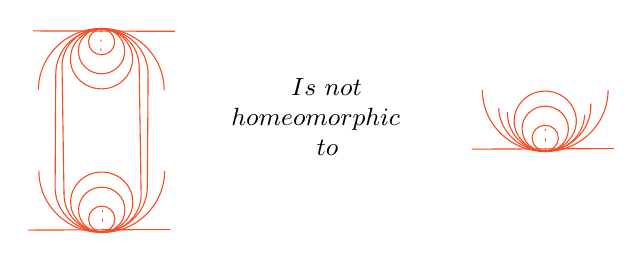
\begin{tikzpicture}[x=0.75pt,y=0.75pt,yscale=-1,xscale=1]
%uncomment if require: \path (0,330); %set diagram left start at 0, and has height of 330

%Shape: Arc [id:dp42777306144239347] 
\draw  [draw opacity=0] (256.41,139.87) .. controls (256.41,139.87) and (256.41,139.87) .. (256.41,139.87) .. controls (256.41,156.24) and (242.86,169.5) .. (226.13,169.5) .. controls (209.4,169.5) and (195.84,156.24) .. (195.84,139.87) -- (226.13,139.87) -- cycle ; \draw  [color={rgb, 255:red, 245; green, 76; blue, 35 }  ,draw opacity=1 ] (256.41,139.87) .. controls (256.41,139.87) and (256.41,139.87) .. (256.41,139.87) .. controls (256.41,156.24) and (242.86,169.5) .. (226.13,169.5) .. controls (209.4,169.5) and (195.84,156.24) .. (195.84,139.87) ;  
%Shape: Arc [id:dp797304877230008] 
\draw  [draw opacity=0] (248.08,146.43) .. controls (248.68,158.35) and (239.22,168.52) .. (226.96,169.13) .. controls (214.69,169.75) and (204.26,160.59) .. (203.66,148.66) -- (225.87,147.55) -- cycle ; \draw  [color={rgb, 255:red, 245; green, 76; blue, 35 }  ,draw opacity=1 ] (248.08,146.43) .. controls (248.68,158.35) and (239.22,168.52) .. (226.96,169.13) .. controls (214.69,169.75) and (204.26,160.59) .. (203.66,148.66) ;  
%Shape: Arc [id:dp8908957957332029] 
\draw  [draw opacity=0] (245.11,151.77) .. controls (244.76,161.81) and (236.15,169.65) .. (225.89,169.29) .. controls (215.63,168.93) and (207.6,160.5) .. (207.96,150.46) -- (226.53,151.12) -- cycle ; \draw  [color={rgb, 255:red, 245; green, 76; blue, 35 }  ,draw opacity=1 ] (245.11,151.77) .. controls (244.76,161.81) and (236.15,169.65) .. (225.89,169.29) .. controls (215.63,168.93) and (207.6,160.5) .. (207.96,150.46) ;  
%Shape: Ellipse [id:dp03680214293557027] 
\draw  [color={rgb, 255:red, 245; green, 76; blue, 35 }  ,draw opacity=1 ] (214.97,158.58) .. controls (214.97,152.55) and (219.96,147.66) .. (226.13,147.66) .. controls (232.29,147.66) and (237.29,152.55) .. (237.29,158.58) .. controls (237.29,164.61) and (232.29,169.5) .. (226.13,169.5) .. controls (219.96,169.5) and (214.97,164.61) .. (214.97,158.58) -- cycle ;
%Shape: Ellipse [id:dp48314716650274747] 
\draw  [color={rgb, 255:red, 245; green, 76; blue, 35 }  ,draw opacity=1 ] (219.81,162.98) .. controls (219.81,159.57) and (222.64,156.8) .. (226.13,156.8) .. controls (229.62,156.8) and (232.45,159.57) .. (232.45,162.98) .. controls (232.45,166.4) and (229.62,169.16) .. (226.13,169.16) .. controls (222.64,169.16) and (219.81,166.4) .. (219.81,162.98) -- cycle ;
%Straight Lines [id:da6993970124426362] 
\draw [color={rgb, 255:red, 245; green, 76; blue, 35 }  ,draw opacity=1 ] [dash pattern={on 0.84pt off 2.51pt}]  (226.46,158.65) -- (226.46,169.57) ;
%Shape: Ellipse [id:dp025809737358414853] 
\draw  [color={rgb, 255:red, 245; green, 76; blue, 35 }  ,draw opacity=1 ] (211.16,154.78) .. controls (211.16,146.83) and (217.86,140.39) .. (226.13,140.39) .. controls (234.4,140.39) and (241.1,146.83) .. (241.1,154.78) .. controls (241.1,162.72) and (234.4,169.16) .. (226.13,169.16) .. controls (217.86,169.16) and (211.16,162.72) .. (211.16,154.78) -- cycle ;
%Straight Lines [id:da6887063203021668] 
\draw [color={rgb, 255:red, 245; green, 76; blue, 35 }  ,draw opacity=1 ]   (190.71,168.34) -- (259.21,168.09) ;
%Shape: Arc [id:dp3693665851394208] 
\draw  [draw opacity=0] (195.62,100.63) .. controls (195.62,100.63) and (195.62,100.63) .. (195.62,100.63) .. controls (195.73,84.26) and (209.37,71.09) .. (226.09,71.19) .. controls (242.82,71.3) and (256.29,84.65) .. (256.19,101.01) -- (225.91,100.82) -- cycle ; \draw  [color={rgb, 255:red, 245; green, 76; blue, 35 }  ,draw opacity=1 ] (195.62,100.63) .. controls (195.62,100.63) and (195.62,100.63) .. (195.62,100.63) .. controls (195.73,84.26) and (209.37,71.09) .. (226.09,71.19) .. controls (242.82,71.3) and (256.29,84.65) .. (256.19,101.01) ;  
%Shape: Arc [id:dp8338437028438305] 
\draw  [draw opacity=0] (203.98,93) .. controls (204.05,81.07) and (214.07,71.45) .. (226.35,71.53) .. controls (238.63,71.61) and (248.53,81.35) .. (248.45,93.28) -- (226.21,93.14) -- cycle ; \draw  [color={rgb, 255:red, 245; green, 76; blue, 35 }  ,draw opacity=1 ] (203.98,93) .. controls (204.05,81.07) and (214.07,71.45) .. (226.35,71.53) .. controls (238.63,71.61) and (248.53,81.35) .. (248.45,93.28) ;  
%Shape: Arc [id:dp8090516680248827] 
\draw  [draw opacity=0] (206.99,89.45) .. controls (207.05,79.41) and (215.42,71.32) .. (225.69,71.39) .. controls (235.95,71.45) and (244.22,79.64) .. (244.16,89.69) -- (225.57,89.57) -- cycle ; \draw  [color={rgb, 255:red, 245; green, 76; blue, 35 }  ,draw opacity=1 ] (206.99,89.45) .. controls (207.05,79.41) and (215.42,71.32) .. (225.69,71.39) .. controls (235.95,71.45) and (244.22,79.64) .. (244.16,89.69) ;  
%Shape: Ellipse [id:dp8978682080533286] 
\draw  [color={rgb, 255:red, 245; green, 76; blue, 35 }  ,draw opacity=1 ] (237.19,82.18) .. controls (237.15,88.21) and (232.12,93.07) .. (225.96,93.03) .. controls (219.79,92.99) and (214.82,88.07) .. (214.86,82.04) .. controls (214.9,76.01) and (219.93,71.15) .. (226.09,71.19) .. controls (232.26,71.23) and (237.22,76.15) .. (237.19,82.18) -- cycle ;
%Shape: Ellipse [id:dp22773855421731792] 
\draw  [color={rgb, 255:red, 245; green, 76; blue, 35 }  ,draw opacity=1 ] (232.37,77.75) .. controls (232.35,81.16) and (229.5,83.91) .. (226.01,83.89) .. controls (222.52,83.87) and (219.71,81.08) .. (219.74,77.67) .. controls (219.76,74.26) and (222.6,71.51) .. (226.09,71.53) .. controls (229.58,71.55) and (232.39,74.34) .. (232.37,77.75) -- cycle ;
%Straight Lines [id:da891993741817402] 
\draw [color={rgb, 255:red, 245; green, 76; blue, 35 }  ,draw opacity=1 ] [dash pattern={on 0.84pt off 2.51pt}]  (225.7,82.04) -- (225.77,71.12) ;
%Shape: Ellipse [id:dp37710316486801587] 
\draw  [color={rgb, 255:red, 245; green, 76; blue, 35 }  ,draw opacity=1 ] (240.97,86.01) .. controls (240.92,93.95) and (234.18,100.35) .. (225.91,100.3) .. controls (217.64,100.24) and (210.98,93.76) .. (211.03,85.82) .. controls (211.08,77.87) and (217.82,71.48) .. (226.09,71.53) .. controls (234.36,71.58) and (241.02,78.06) .. (240.97,86.01) -- cycle ;
%Straight Lines [id:da13911890461318233] 
\draw [color={rgb, 255:red, 245; green, 76; blue, 35 }  ,draw opacity=1 ]   (261.5,72.57) -- (193,72.39) ;
%Straight Lines [id:da14513158759358802] 
\draw [color={rgb, 255:red, 245; green, 76; blue, 35 }  ,draw opacity=1 ]   (206.99,89.45) -- (207.95,151.12) ;
%Straight Lines [id:da8217624934121862] 
\draw [color={rgb, 255:red, 245; green, 76; blue, 35 }  ,draw opacity=1 ]   (244.16,89.45) -- (245.11,151.77) ;
%Straight Lines [id:da3194167754893965] 
\draw [color={rgb, 255:red, 245; green, 76; blue, 35 }  ,draw opacity=1 ]   (203.98,93) -- (203.66,148.66) ;
%Straight Lines [id:da04274569390948202] 
\draw [color={rgb, 255:red, 245; green, 76; blue, 35 }  ,draw opacity=1 ]   (248.45,93) -- (248.11,147.55) ;
%Shape: Arc [id:dp23804029242995062] 
\draw  [draw opacity=0] (470.08,100.87) .. controls (470.08,100.87) and (470.08,100.87) .. (470.08,100.87) .. controls (470.08,117.24) and (456.52,130.5) .. (439.8,130.5) .. controls (423.07,130.5) and (409.51,117.24) .. (409.51,100.87) .. controls (409.51,100.87) and (409.51,100.87) .. (409.51,100.87) -- (439.8,100.87) -- cycle ; \draw  [color={rgb, 255:red, 245; green, 76; blue, 35 }  ,draw opacity=1 ] (470.08,100.87) .. controls (470.08,100.87) and (470.08,100.87) .. (470.08,100.87) .. controls (470.08,117.24) and (456.52,130.5) .. (439.8,130.5) .. controls (423.07,130.5) and (409.51,117.24) .. (409.51,100.87) .. controls (409.51,100.87) and (409.51,100.87) .. (409.51,100.87) ;  
%Shape: Arc [id:dp36122789927787213] 
\draw  [draw opacity=0] (461.75,107.43) .. controls (462.35,119.35) and (452.89,129.52) .. (440.62,130.13) .. controls (428.36,130.75) and (417.93,121.59) .. (417.33,109.66) -- (439.54,108.55) -- cycle ; \draw  [color={rgb, 255:red, 245; green, 76; blue, 35 }  ,draw opacity=1 ] (461.75,107.43) .. controls (462.35,119.35) and (452.89,129.52) .. (440.62,130.13) .. controls (428.36,130.75) and (417.93,121.59) .. (417.33,109.66) ;  
%Shape: Arc [id:dp6957683654314288] 
\draw  [draw opacity=0] (458.78,112.77) .. controls (458.78,112.77) and (458.78,112.77) .. (458.78,112.77) .. controls (458.42,122.81) and (449.82,130.65) .. (439.56,130.29) .. controls (429.3,129.93) and (421.27,121.5) .. (421.62,111.46) -- (440.2,112.12) -- cycle ; \draw  [color={rgb, 255:red, 245; green, 76; blue, 35 }  ,draw opacity=1 ] (458.78,112.77) .. controls (458.78,112.77) and (458.78,112.77) .. (458.78,112.77) .. controls (458.42,122.81) and (449.82,130.65) .. (439.56,130.29) .. controls (429.3,129.93) and (421.27,121.5) .. (421.62,111.46) ;  
%Shape: Ellipse [id:dp5800282561343184] 
\draw  [color={rgb, 255:red, 245; green, 76; blue, 35 }  ,draw opacity=1 ] (428.63,119.58) .. controls (428.63,113.55) and (433.63,108.66) .. (439.8,108.66) .. controls (445.96,108.66) and (450.96,113.55) .. (450.96,119.58) .. controls (450.96,125.61) and (445.96,130.5) .. (439.8,130.5) .. controls (433.63,130.5) and (428.63,125.61) .. (428.63,119.58) -- cycle ;
%Shape: Ellipse [id:dp48549178458764863] 
\draw  [color={rgb, 255:red, 245; green, 76; blue, 35 }  ,draw opacity=1 ] (433.48,123.98) .. controls (433.48,120.57) and (436.31,117.8) .. (439.8,117.8) .. controls (443.28,117.8) and (446.11,120.57) .. (446.11,123.98) .. controls (446.11,127.4) and (443.28,130.16) .. (439.8,130.16) .. controls (436.31,130.16) and (433.48,127.4) .. (433.48,123.98) -- cycle ;
%Straight Lines [id:da22581486450821575] 
\draw [color={rgb, 255:red, 245; green, 76; blue, 35 }  ,draw opacity=1 ] [dash pattern={on 0.84pt off 2.51pt}]  (440.12,119.65) -- (440.12,130.57) ;
%Shape: Ellipse [id:dp01793013294843626] 
\draw  [color={rgb, 255:red, 245; green, 76; blue, 35 }  ,draw opacity=1 ] (424.83,115.78) .. controls (424.83,107.83) and (431.53,101.39) .. (439.8,101.39) .. controls (448.06,101.39) and (454.77,107.83) .. (454.77,115.78) .. controls (454.77,123.72) and (448.06,130.16) .. (439.8,130.16) .. controls (431.53,130.16) and (424.83,123.72) .. (424.83,115.78) -- cycle ;
%Straight Lines [id:da429409746243253] 
\draw [color={rgb, 255:red, 245; green, 76; blue, 35 }  ,draw opacity=1 ]   (404.38,129.34) -- (472.88,129.09) ;

% Text Node
\draw (280.67,91.73) node [anchor=north west][inner sep=0.75pt]  [font=\small]  {$ \begin{array}{l}
\ \ \ \ \ \ \ Is\ not\ \\
homeomorphic\ \\
\ \ \ \ \ \ \ \ \ \ to
\end{array}$};


\end{tikzpicture}


\end{center}\pause
And as it is path connected, it can't be broken in two homeomorphic open sets.\pause Therefore \textcolor{colororange}{$\phi\circ \psi$} is not a covering of \textcolor{colororange}{$X$} by \textcolor{colororange}{$Z$}. 
\end{frame}


\begin{frame}{References}
\begin{itemize}
    \item Hatcher, Allen. Algebraic Topology. 2001, https://doi.org/10.1604/9780521795401.
\end{itemize}
    
\end{frame}

\end{document}